%%%% Шаблон ВКР <<SPbPU-student-thesis-template>>  %%%%
%%
%%   Создан на основе глубокой переработки шаблона российских кандидатских и докторских диссертаций [1]. 
%%   
%%   Полный список различий может быть получен командами git.
%%   Лист авторов-составителей расположен в README.md файле.
%%   Подробные инструкции по использованию в [1,2].
%%   
%%   Рекомендуем установить TeX Live + TeXstudio
%%   <<Стандартная>> компиляция 2-3 РАЗА с помощью pdflatex + biber (для библиографии)     
%%  
%%%% Student thesis template <<SPbPU-student-thesis-template>> %%%%
%%
%%   Created on the basis of deepl modifification of the Russian candidate and doctorate thesis template [1]. 
%%   
%%   Full list of differences can be achieved by git commands.
%%   List of template authors can be seen in the README.md file.
%%   Detailed instructions of usage, see, please in [1,2].
%%     
%%   [1] github.com/AndreyAkinshin/Russian-Phd-LaTeX-Dissertation-Template 
%%   [2] Author_guide_SPBPU-student-thesis-template.pdf
%%   
%%   It is recommended to install TeX Live + TeXstudio   
%%   Default compilation 2-3 TIMES with pdflatex + biber (for the bibliography)
%%  
%%%% Preamble start %%%%  
%%
%%   Please, do not modify files in the preamble
%%
\newcommand*{\anyptfilebase}{template_settings/bpfont} 
\newcommand*{\anyptsize}{14} 		 
\RequirePackage[l2tabu,orthodox]{nag} 
\documentclass[extrafontsizes,a4paper,*pt,oneside,openany]{memoir}
%%%%%%%%%%%%%%%%%%%%%%%%%%%%%%%%%%%%%%%%%%%%%%%%%%%%%%
%%%% Файл упрощённых настроек шаблона диссертации %%%%
%%%%%%%%%%%%%%%%%%%%%%%%%%%%%%%%%%%%%%%%%%%%%%%%%%%%%%

%%% Инициализирование переменных, не трогать!  %%%
\newcounter{intvl}
\newcounter{otstup}
\newcounter{contnumeq}
\newcounter{contnumfig}
\newcounter{contnumtab}
\newcounter{pgnum}
\newcounter{chapstyle}
\newcounter{headingdelim}
\newcounter{headingalign}
\newcounter{headingsize}
\newcounter{tabcap}
\newcounter{tablaba}
\newcounter{tabtita}
\newcounter{docType} 		% тип документа
\newcounter{tskPrint} 		% печать Задания на ВКР двух(одно)сторонняя
\newcounter{tskPages}       % для учёта количества страниц в Задании
\newcounter{tskPageFirst}   % для учёта количества страниц в Задании
\newcounter{tskPageLast}    % для учёта количества страниц в Задании 
\newcounter{sumPrint} 		% печать Реферата на ВКР двух(одно)сторонняя
\newcounter{sumPages}       % для учёта количества страниц в Реферате
\newcounter{sumPageFirst}   % для учёта количества страниц в Реферате
\newcounter{sumPageLast}    % для учёта количества страниц в Реферате 
\newcommand{\Single}{0.78}  % пропорция для одинароного отступа в \Spacing
%%%%%%%%%%%%%%%%%%%%%%%%%%%%%%%%%%%%%%%%%%%%%%%%%%

%%% Область упрощённого управления оформлением %%%

% Управление перенесено в главые файлы компиляции ВКР, Задания, Реферата
\setcounter{tskPrint}{0} %по умолчанию односторонняя печать              
%\setcounter{sumPrint}{0} %по умолчанию односторонняя печать 

%% Интервал между заголовками и между заголовком и текстом
% Заголовки отделяют от текста сверху и снизу тремя интервалами (ГОСТ Р 7.0.11-2011, 5.3.5)
\setcounter{intvl}{3}               % Коэффициент кратности к размеру шрифта

% Заголовки отделяют от текста сверху и снизу тремя интервалами 
\newcommand{\intvlS}{1.5}               % Коэффициент кратности к размеру шрифта SPbPU-student-templates

\newcommand{\intervalS}{\vspace{\intvlS\curtextsize}}

% печать списка источников в Задании
\newcommand{\printbibliographyTask}{\vspace{-0.28\curtextsize}
	\printbibliography[env=tsk] % печать списка литературы в исходных данных
	\vspace{-0.28\curtextsize}}


%% Отступы у заголовков в тексте
\setcounter{otstup}{0}              % 0 --- без отступа; 1 --- абзацный отступ

%% Нумерация формул, таблиц и рисунков
\setcounter{contnumeq}{0}           % Нумерация формул: 0 --- пораздельно (во введении подряд, без номера раздела); 1 --- сквозная нумерация по всей диссертации
\setcounter{contnumfig}{0}          % Нумерация рисунков: 0 --- пораздельно (во введении подряд, без номера раздела); 1 --- сквозная нумерация по всей диссертации
\setcounter{contnumtab}{0}          % Нумерация таблиц: 0 --- пораздельно (во введении подряд, без номера раздела); 1 --- сквозная нумерация по всей диссертации


%% Нумерация подстраничных сносок (ссылок)
%сквозная
\counterwithout{footnote}{chapter} %сквозная нумерация подразделов (во всех главах)


%% Нумерация подразделов
%убрать номер главы в секции
%\counterwithout{section}{chapter} %сквозная нумерация подразделов (во всех главах)
%\renewcommand\thesection{\arabic{section}} %в каждой главе нумерация заново

%\renewcommand\thesection{\arabic{section}}
%\renewcommand\thefigure{\fbox{\arabic{figure}}}
%\renewcommand\thetable{\arabic{table}}
%\renewcommand\theequation{\arabic{equation}}



%\counterwithout{section}{chapter}
%\counterwithout{figure}{chapter}
%\counterwithout{table}{chapter}
%\counterwithout{equation}{chapter}

%\counterwithin{section}{chapter}
%\counterwithin{figure}{chapter}
%\counterwithin{table}{chapter}

%% Оглавление

\setcounter{pgnum}{1}               %NB УДАЛЕНО ФИЗИЧЕСКИ 0 --- номера страниц никак не обозначены; 1 --- Стр. над номерами страниц (дважды компилировать после изменения)  
\settocdepth{subsection} %             до какого уровня подразделов выносить в оглавление
\setsecnumdepth{subsubsection}         % до какого уровня нумеровать подразделы


%% Текст и форматирование заголовков
\setcounter{chapstyle}{1}           % 0 --- разделы только под номером; 1 --- разделы с названием "Глава" перед номером
\setcounter{headingdelim}{2}        % 0 --- номер отделен пропуском в 1em или \quad; 1 --- номера разделов и ений отделены точкой с пробелом, подразделы пропуском без точки; 2 --- номера разделов, подразделов и приложений отделены точкой с пробелом.

%% Выравнивание заголовков в тексте
\setcounter{headingalign}{0}        % 0 --- по центру; 1 --- по левому краю

%% Размеры заголовков в тексте
\setcounter{headingsize}{0}         % 0 --- SPbPU style, все всегда 14 пт; 1 --- пропорционально изменяющийся размер в зависимости от базового шрифта;

%% Подпись таблиц
\setcounter{tabcap}{1}              % 0 --- по ГОСТ, номер таблицы и название разделены тире, выровнены по левому краю, при необходимости на нескольких строках; 1 --- подпись таблицы не по ГОСТ, на двух и более строках, дальнейшие настройки: 
%Выравнивание первой строки, с подписью и номером
\setcounter{tablaba}{2}             % 0 --- по левому краю; 1 --- по центру; 2 --- по правому краю
%Выравнивание строк с самим названием таблицы
\setcounter{tabtita}{1}             % 0 --- по левому краю; 1 --- по центру; 2 --- по правому краю
%Разделитель записи «Таблица #» и названия таблицы
\newcommand{\tablabelsep}{space}   % space = пробел, period =  (определены в подключенных пакетах)

%% Подпись рисунков
%Разделитель записи «Рисунок #» и названия рисунка
\newcommand{\figlabelsep}{period}   % emdash = тире, определён в common/styles; period = точка определён в подключенных пакетах; space
%\newcommand{\figlabelsep}{emdash}   % emdash = тире, определён в common/styles; period = точка определён в подключенных пакетах


%%% Цвета гиперссылок %%%
% Latex color definitions: http://latexcolor.com/

%\definecolor{linkcolor}{rgb}{0.9,0,0}
%\definecolor{citecolor}{rgb}{0,0.6,0}
%\definecolor{urlcolor}{rgb}{0,0,1}


%\definecolor{linkbordercolor}{rgb}{0,0,1}

\definecolor{linkcolor}{HTML}{FF0000} %very light red from the SPbPU brandbook (2nd level)
\definecolor{citecolor}{HTML}{6CF479} %very light green from the SPbPU brandbook (2nd level)
\definecolor{urlcolor}{HTML}{4481BA} %very light blue from the SPbPU brandbook (2nd level)

%\definecolor{linkcolor}{rgb}{0,0,0} %black
%\definecolor{citecolor}{rgb}{0,0,0} %black
%\definecolor{urlcolor}{rgb}{0,0,0} %black               
%%% Проверка используемого TeX-движка %%%
\usepackage{iftex}[2013/04/04]
\newif\ifxetexorluatex   % определяем новый условный оператор (http://tex.stackexchange.com/a/47579/79756)
\ifXeTeX
    \xetexorluatextrue
\else
    \ifLuaTeX
        \xetexorluatextrue
    \else
        \xetexorluatexfalse
    \fi
\fi

\RequirePackage{etoolbox}[2015/08/02]               % Для продвинутой проверки разных условий

%%% Поля и разметка страницы %%%

\usepackage{pdflscape}                              % Для включения альбомных страниц
\usepackage{geometry}                               % Для последующего задания полей

%%% Математические пакеты %%%
\usepackage{amsfonts,amsmath,amssymb,amscd,amsthm}  % Математические дополнения от AMS
% %amsthm should be loaded after amsmath!!

\usepackage{mathtools}                              % Добавляет окружение multlined

%%%% Установки для размера шрифта 14 pt %%%%
%% Формирование переменных и констант для сравнения (один раз для всех подключаемых файлов)%%
%% должно располагаться до вызова пакета fontspec или polyglossia, потому что они сбивают его работу
\newlength{\curtextsize}
\newlength{\bigtextsize}
\setlength{\bigtextsize}{13.9pt}

\makeatletter
%\show\f@size                                       % неплохо для отслеживания, но вызывает стопорение процесса, если документ компилируется без команды  -interaction=nonstopmode 
\setlength{\curtextsize}{\f@size pt}
\makeatother

% %%% Кодировки и шрифты %%%
% \ifxetexorluatex
%     \usepackage{polyglossia}[2014/05/21]            % Поддержка многоязычности (fontspec подгружается автоматически)
% \else
%     \RequirePDFTeX                                  % tests for PDFTEX use and throws an error if a different engine is being used
%    %%% Решение проблемы копирования текста в буфер кракозябрами
% %    \input glyphtounicode.tex
% %    \input glyphtounicode-cmr.tex %from pdfx package
% %    \pdfgentounicode=1
%     \usepackage{cmap}                               % Улучшенный поиск русских слов в полученном pdf-файле
%     \defaulthyphenchar=127                          % Если стоит до fontenc, то переносы не впишутся в выделяемый текст при копировании его в буфер обмена
    
% %    \usepackage[T2A]{fontenc}                       % Поддержка русских букв
%     \usepackage[T2A,T1]{fontenc}
%     \usepackage[utf8]{inputenc}[2014/04/30]         % Кодировка utf8
%     \usepackage[english, russian]{babel}[2014/03/24]% Языки: русский, английский
% \fi
% \usepackage{tempora} %TemporaLGCUni of Times type
% \usepackage{newtxmath} %math font of Times type
% % need to set the monospace=typewritter font
% %https://tex.stackexchange.com/questions/213835/using-many-typewriter-fonts-in-a-single-document
\usepackage{fontspec, lipsum}
\usepackage[utf8]{inputenc}
\usepackage[T1,T2A]{fontenc}
\usepackage{textcomp}
\usepackage[english, russian]{babel}

% Математические шрифты как в LaTeX
% \DeclareMathAlphabet{\mathcal}{OMS}{cmsy}{m}{n}
% \let\mathbb\relax % remove the definition by unicode-math
% \DeclareMathAlphabet{\mathbb}{U}{msb}{m}{n}

% % Шрифты документа (текст)
% \setmainfont[Ligatures=TeX]{CMU Serif} % обычный текст
\setmainfont[Ligatures=TeX]{Times New Roman} % обычный текст
% \setmonofont{Fira Code Regular} % код



\makeatletter %load fonts for cmtt
\providecommand{\EC@ttfamily}[5]{%
	\DeclareFontShape{#1}{#2}{#3}{#4}{
		<-8.5>#50800
		<8.5-9.5>#50900
		<9.5-10.5>#51000
		<10.5-11.5>#51095
		<11.5-13>#51200
		<13-15.5>#51440
		<15.5-18.5>#51728
		<18.5-22>#52074
		<22-27>#52488
		<27-32>#52986
		<32->#53583}{}}
\DeclareFontFamily{T1}{cmtt}{}
\DeclareFontFamily{T2A}{cmtt}{}
\EC@ttfamily{T1}{cmtt}{m}{n}{ectt}
\EC@ttfamily{T1}{cmtt}{m}{sl}{ecst}
\EC@ttfamily{T1}{cmtt}{m}{it}{ecit}
\EC@ttfamily{T1}{cmtt}{m}{sc}{ectc}
\DeclareFontShape{T1}{cmtt}{bx}{n}%
{<->ssub*cmtt/m/n}{}
\DeclareFontShape{T1}{cmtt}{bx}{it}%
{<->ssub*cmtt/m/it}{}
\EC@ttfamily{T2A}{cmtt}{m}{n}{latt}
\EC@ttfamily{T2A}{cmtt}{m}{sl}{last}
\EC@ttfamily{T2A}{cmtt}{m}{it}{lait}
\EC@ttfamily{T2A}{cmtt}{m}{sc}{latc}
\DeclareFontShape{T2A}{cmtt}{bx}{n}%
{<->ssub*cmtt/m/n}{}
\DeclareFontShape{T2A}{cmtt}{bx}{it}%
{<->ssub*cmtt/m/it}{}
\makeatletter

%\makeatletter %load fonts for cmtt
%\providecommand{\EC@ttfamily}[5]{%
%	\DeclareFontShape{#1}{#2}{#3}{#4}{
%		<-8.5>#50800
%		<8.5-9.5>#50900
%		<9.5-10.5>#51000
%		<10.5-11.5>#51095
%		<11.5-13>#51200
%		<13-15.5>#51440
%		<15.5-18.5>#51728
%		<18.5-22>#52074
%		<22-27>#52488
%		<27-32>#52986
%		<32->#53583}{}}
%\DeclareFontFamily{T2A}{cmtt}{\hyphenchar\font\m@ne}
%\EC@ttfamily{T2A}{cmtt}{m}{n}{latt}
%\EC@ttfamily{T2A}{cmtt}{m}{sl}{last}
%\EC@ttfamily{T2A}{cmtt}{m}{it}{lait}
%\EC@ttfamily{T2A}{cmtt}{m}{sc}{latc}
%\DeclareFontShape{T2A}{cmtt}{bx}{n}%
%{<->ssub*cmtt/m/n}{}
%\DeclareFontShape{T2A}{cmtt}{bx}{it}%
%{<->ssub*cmtt/m/it}{}
%\makeatletter

%\makeatletter
%\input{t1lmtt.fd}
%\@namedef{T1+lmtt}{}
%\makeatother


\renewcommand{\ttdefault}{cmtt}
%\renewcommand{\ttdefault}{lcmtt} %покрупнее
%\usepackage[scaled=.85]{DejaVuSansMono} %слишком похож на рубленый
%\newfont{\wasyten}{wasy10} %название команды для вызова / название шрифта



%Другие шрифты:
% математика
%\usepackage[lite]{mtpro2}
%https://pctex.com/mtpro2.html
% текст        
% https://www.ctan.org/pkg/paratype
%       \usepackage[scaled=0.925]{XCharter}[2017/06/25] % Подключение русифицированных шрифтов XCharter
%\usepackage{pscyr}
%    \IfFileExists{pscyr.sty}{}{}  % Красивые русские шрифты
%\fi

%https://tex.stackexchange.com/questions/8260/what-are-the-various-units-ex-em-in-pt-bp-dd-pc-expressed-in-mm
\usepackage{printlen} %для измерения и вывода параменторов шрифтов, отступов, интервалов

\usepackage{bm} %для жирных начертаний символов

\usepackage{csquotes} %to check quotes

%%% Оформление абзацев %%%
\usepackage{indentfirst}                            % Красная строка

%%% Цвета %%%
%\usepackage[dvipsnames,usenames]{color}
\usepackage{colortbl}
\usepackage[dvipsnames, table, hyperref, cmyk]{xcolor} % Вероятно, более новый вариант, вместо предыдущих двух строк. Конвертация всех цветов в cmyk заложена как удовлетворение возможного требования типографий. Возможно конвертирование и в rgb.

%%% Таблицы %%%
\usepackage{longtable}                              % Длинные таблицы
\usepackage{multirow,makecell}                      % Улучшенное форматирование таблиц:
													% multirow - строки на несколько ячеек, 
												
													% makecell - сесколько строк в ячейке.
													% не работает, если внутри, например, \verb|text| -> \texttt{text}
													% аналоги
%https://tex.stackexchange.com/questions/2441/how-to-add-a-forced-line-break-inside-a-table-cell								
						
													

%%% Общее форматирование
%\usepackage{soul} % используется ulem
\usepackage{soulutf8}                               % Поддержка переносоустойчивых подчёркиваний и зачёркиваний
\usepackage{icomma}                                 % Запятая в десятичных дробях



%%% Предметный указатель  ГОСТ 7.78-99 Index %%%
%c обобщенными рубриками или развернутый
%или указатель терминов (в общем случае - произвольное число указателей)
%подключать до hyperref

%\usepackage{makeidx} %возможно, необходимо подключить И/ИЛИ пройти Tools-> Commands -> MakeIndex

\usepackage{imakeidx} 
%\indexsetup{level=\section*,toclevel=section,noclearpage}
\makeindex[program=makeindex,
options=-s template_settings/common/myindex.ist, %подключаем стилевой файл для форматирования вывода
name=ru, % префикс для русских указателей 
% если убрать <<ru>>, то для работы дефолтового придется вручную включать Tools-> Commands -> MakeIndex
title={\chapterLight{} 
%   \hrule{}
	Предметный указатель
%	\hrule{}
} 
%,columns=1 %по умолчанию 2
]
\makeindex[program=makeindex,
options=-s template_settings/common/myindex.ist, %подключаем стилевой файл для форматирования вывода
name=en, % префикс для английских указателей
title={\chapterLight{}
%	\hrule{}
	Index
%	\hrule{}
} 
%,columns=1 %по умолчанию 2
] 
%убрать добавление <<title>> в содержание:
%\noindexintoc %not to add index title in PURE makeidx %intoc is false by default with imakeidx


%       https://tex.stackexchange.com/a/132415/44348
%\makeatletter
%% we want hyphenation also in the first word
\renewcommand{\@idxitem}{\par\hangindent40\p@\hspace{0pt}\ignorespaces}
%% we don't want a page break before a subitem %implemented in the previous one
%%\renewcommand\subitem{\@idxitem\nobreak\hspace*{20\p@}}
%\makeatother


%%% Фиксация плавающих объектов





%%% Гиперссылки %%%
\usepackage{hyperref}[2012/11/06]

%%% Изображения %%%
\usepackage{graphicx}[2014/04/25]                   % Подключаем пакет работы с графикой

%%% Списки %%%
\usepackage[shortlabels]{enumitem} % shortlabels для того, чтобы изменять токены в списках с дефолтных (иерархическая структура) на произвольныею

%%% Подписи %%%
\usepackage{caption}[2013/05/02]                    % Для управления подписями (рисунков и таблиц) % Может управлять номерами рисунков и таблиц с caption %Иногда может управлять заголовками в списках рисунков и таблиц


\usepackage{subcaption}[2013/02/03]                 % Работа с подрисунками и подобным

%%% Счётчики %%%
%\usepackage[figure,table]{totalcount}               % Счётчик рисунков и таблиц. Взамен используется xassoccnt 
\usepackage{totcount}                               % Пакет создания счётчиков на основе последнего номера подсчитываемого элемента (может требовать дважды компилировать документ)
\usepackage{totpages}                               % Счётчик страниц, совместимый с hyperref (ссылается на номер последней страницы). Желательно ставить последним пакетом в преамбуле

\usepackage{xassoccnt} % для подсчета сумм приложений, рисунков, таблиц 


%%% Продвинутое управление групповыми ссылками (пока только формулами) %%%
\ifxetexorluatex
    \usepackage{cleveref}                           % cleveref корректно считывает язык из настроек polyglossia
\else
    \usepackage[russian]{cleveref}                  % cleveref имеет сложности со считыванием языка из babel. Такое решение русификации вывода выбрано вместо определения в documentclass из опасности что-то лишнее передать во все остальные пакеты, включая библиографию.
\fi
\creflabelformat{equation}{#2#1#3}                  % Формат по умолчанию ставил круглые скобки вокруг каждого номера ссылки, теперь просто номера ссылок без какого-либо дополнительного оформления



\ifnumequal{\value{draft}}{1}{% Черновик
    \usepackage[firstpage]{draftwatermark}
    \SetWatermarkText{DRAFT}
    \SetWatermarkFontSize{14pt}
    \SetWatermarkScale{15}
    \SetWatermarkAngle{45}
}{}

  
%%% Прикладные пакеты %%% 
%\usepackage{calc}               % Пакет для расчётов параметров, например длины

%%% Для добавления Стр. над номерами страниц в оглавлении
%%% http://tex.stackexchange.com/a/306950
\usepackage{afterpage}

\urlstyle{rm} % links in Times


%\makeatletter
%%расстояние после ToC title до 1ой строчки 
%%для достижения одинаковых отсупов переопределено формирование базового ToC
%\renewcommand{\aftertoctitle}{\par\nobreak\vskip1\curtextsize}
%\makeatother

%https://tex.stackexchange.com/questions/170912/contents-page-in-two-different-languages
%\makeatletter
\newcommand\russiantableofcontents{%
%	\if@twocolumn
%	\@restonecoltrue\onecolumn
%	\else
%	\@restonecolfalse
%	\fi
	%  \begin{otherlanguage}{russian}
	\chapter*{%
	\normalfont\MakeUppercase{Содержание} %слово <<Содержание>> в стилю chaperLight, по факту убираем \bfseries
%		    \contentsname
%		    \@mkboth{\MakeUppercaseСодержание}
%		            {\MakeUppercaseСодержание}%
	}%
%\hrule
\vspace*{-1\curtextsize} %убрать лишний отступ в таблице
	\@starttoc{tuc}%
	%  \end{otherlanguage}
%	\if@restonecol\twocolumn\fi
}
\newcommand{\addtocru}[2]{%
	\addcontentsline{tuc}{#1}{\protect\numberline{\csname the#1\endcsname}#2}%
%	\addcontentsline{tuc}{#1}{#2}%
}
\newcommand{\addtocruNoProtect}[2]{%
%	\addcontentsline{tuc}{#1}{\protect\numberline{\csname the#1\endcsname}#2}%
		\addcontentsline{tuc}{#1}{#2}%
}

%обеспечение красивого порядка вывода содержаний и названий разделов, подразделов и т.п.
\newcommand\englishtableofcontents{%
	%	\if@twocolumn
	%	\@restonecoltrue\onecolumn
	%	\else
	%	\@restonecolfalse
	%	\fi
	%  \begin{otherlanguage}{russian}
	\chapter*{%
		\normalfont\MakeUppercase{Content} %слово <<Содержание>> в стилю chaperLight, по факту убираем \bfseries
		%		    \contentsname
		%		    \@mkboth{\MakeUppercaseСодержание}
		%		            {\MakeUppercaseСодержание}%
	}%
	%\hrule
	\vspace*{-1\curtextsize} %убрать лишний отступ в таблице
	\@starttoc{tec}%
	%  \end{otherlanguage}
	%	\if@restonecol\twocolumn\fi
}
\newcommand{\addtocen}[2]{%
		\addcontentsline{tec}{#1}{\protect\numberline{\csname the#1\endcsname}#2}%
%	\addcontentsline{tec}{#1}{#2}%
}
\newcommand{\addtocenNoProtect}[2]{%for preface, introduction etc
%	\addcontentsline{tec}{#1}{\protect\numberline{\csname the#1\endcsname}#2}%
		\addcontentsline{tec}{#1}{#2}%
}


%стандартный вывод в toc можно использовать, если издание только на английском или русском.
%переопределена, чтобы обеспечить одинаковые отсупы от названия ToC (toc, tec, tuc) до первой строки
\renewcommand\tableofcontents{%
	%	\if@twocolumn
	%	\@restonecoltrue\onecolumn
	%	\else
	%	\@restonecolfalse
	%	\fi
	%  \begin{otherlanguage}{russian}
	\chapter*{%
		\MakeUppercase{Содержание} %слово <<Содержание>> 
		%		    \contentsname
		%		    \@mkboth{\MakeUppercaseСодержание}
		%		            {\MakeUppercaseСодержание}%
	}%
	%\hrule
%	\vspace*{-0.58\curtextsize} %убрать/добавить отступ от таблицы
	\@starttoc{toc}%
	%  \end{otherlanguage}
	%	\if@restonecol\twocolumn\fi
}
\newcommand{\addetoc}[2]{%
		\addcontentsline{toc}{#1}{\protect\numberline{\csname the#1\endcsname}#2}%
}
%\newcommand{\addtocru}[2]{%
%	\addcontentsline{tuc}{#1}{\protect\numberline{\csname the#1\endcsname}#2}%
%	%	\addcontentsline{tuc}{#1}{#2}%
%}

%\makeatother

%http://latex.org/forum/viewtopic.php?t=5438         
\usepackage{tabularx}

%%https://tex.stackexchange.com/a/362229
\usepackage{datatool-base}
\usepackage{mfirstuc} %первая буква прописная

\usepackage{layouts}

\newenvironment{abstr}{\smallA\itshape}{\normalfont\normalsize}


\usepackage[normalem]{ulem} % для перечеркнутых сроков команда \sout{text}
\newcommand{\soutthick}[1]{%
	\renewcommand{\ULthickness}{2.4pt}%
	\sout{#1}%
	\renewcommand{\ULthickness}{.4pt}% Resetting to ulem default
}

%для подчёркнутых команд
%https://tex.stackexchange.com/questions/270286/uline-not-work-for-command-arguments
\useunder{\uline}{\ulined}{}

\usepackage{environ} % for Uppercase in Keywords
%https://tex.stackexchange.com/questions/249628/uppercase-whole-newenvironment
% недостаток - новые окружения не подхватываются TexStudio

\usepackage{textcase} % for \MakeTextUppercase

%for svg pictures
%\usepackage{svg}


%%% Mailto %%% 
%%%https://tex.stackexchange.com/questions/128424/how-to-create-email-hyperlink-with-predefined-subject-in-latex
%% unfortunatelly Adobe does not handle Recipient name + email, e.g.
%% Vladimir Parkhomenko<parhomenko.v@gmail.com>


%mailto with subject (impossible with href)
%mailto anybody without email body
\makeatletter
\newcommand\mailtoab[3]{%                %\newcommand\tpj@compose@mailto[3]{%
	\edef\@tempa{mailto:#1?subject=#2 }%
	\edef\@tempb{\expandafter\html@spaces\@tempa\@empty}%
	\href{\@tempb}{#3}}
\catcode\%=11
\def\html@spaces#1 #2{#1%20\ifx#2\@empty\else\expandafter\html@spaces\fi#2}
	\catcode\%=14
	\makeatother
	
	
	%${email}{Subject}{email start body}{text in pdf}
	\makeatletter
	\newcommand\mailto[4]{%                %\newcommand\tpj@compose@mailto[3]{%
		\edef\@tempa{mailto:#1?subject=#2\&body=#3 }%
		\edef\@tempb{\expandafter\html@spaces\@tempa\@empty}%
		\href{\@tempb}{#4}}
	%% with %20 instead of spaces
	%\catcode\%=11
	%\def\html@spaces#1 #2{#1%20\ifx#2\@empty\else\expandafter\html@spaces\fi#2}
	%\catcode\%=14
	\makeatother
	
	%% MLABSED 2017 author
	%%${email}{Subject}{email start body}{text in pdf}
	\makeatletter
	\newcommand\mailtoMLABSEDauthor[3]{%                
		\edef\@tempa{mailto:#1?subject=MLABSED 2017\&body=#2 }%
		\edef\@tempb{\expandafter\html@spaces\@tempa\@empty}%
		\href{\@tempb}{#3}}
	%% with %20 instead of spaces
	%\catcode\%=11
	%\def\html@spaces#1 #2{#1%20\ifx#2\@empty\else\expandafter\html@spaces\fi#2}
	%\catcode\%=14
	\makeatother
	
	
	%%Vladimir Parkhomenko
	\makeatletter
	\newcommand\mailtopa[1]{%                %\newcommand\tpj@compose@mailto[3]{%
		\edef\@tempa{mailto:parhomenko.v@gmail.com?subject=#1\&body=Dear Vladimir, }%
		\edef\@tempb{\expandafter\html@spaces\@tempa\@empty}%
		\href{\@tempb}{Vladimir.Parkhomenko@spbstu.ru}}
	\catcode\%=11
	\def\html@spaces#1 #2{#1%20\ifx#2\@empty\else\expandafter\html@spaces\fi#2}
		\catcode\%=14
		\makeatother
		
		%%Alexey Buzmakov
		\makeatletter
		\newcommand\mailtobu[1]{%                %\newcommand\tpj@compose@mailto[3]{%
			\edef\@tempa{mailto:abuzmakov@gmail.com?subject=#1\&body=Dear Alexey, }%
			\edef\@tempb{\expandafter\html@spaces\@tempa\@empty}%
			\href{\@tempb}{abuzmakov@gmail.com}}
		\catcode\%=11
		\def\html@spaces#1 #2{#1%20\ifx#2\@empty\else\expandafter\html@spaces\fi#2}
			\catcode\%=14
			\makeatother
			
			%%Xenia Naidenova
			\makeatletter
			\newcommand\mailtona[1]{%                %\newcommand\tpj@compose@mailto[3]{%
				\edef\@tempa{mailto:ksennaidd@gmail.com?subject=#1\&body=Dear Xenia, }%
				\edef\@tempb{\expandafter\html@spaces\@tempa\@empty}%
				\href{\@tempb}{ksennaidd@gmail.com}}
			\catcode\%=11
			\def\html@spaces#1 #2{#1%20\ifx#2\@empty\else\expandafter\html@spaces\fi#2}
				\catcode\%=14
				\makeatother
				
				
				%%Konstantin Shvetsov
				\makeatletter
				\newcommand\mailtosh[1]{%                %\newcommand\tpj@compose@mailto[3]{%
					\edef\@tempa{mailto:shvetsov@inbox.ru?subject=#1\&body=Dear Konstantin, }%
					\edef\@tempb{\expandafter\html@spaces\@tempa\@empty}%
					\href{\@tempb}{Konstantin.Shvetsov@spbstu.ru}}
				\catcode\%=11
				\def\html@spaces#1 #2{#1%20\ifx#2\@empty\else\expandafter\html@spaces\fi#2}
					\catcode\%=14
					\makeatother


\usepackage{tabu, tabulary}  %таблицы с автоматически подбирающейся шириной столбцов
\usepackage{fr-longtable}    %ради \endlasthead

% Листинги с исходным кодом программ
\usepackage{fancyvrb}
\usepackage{listings}
\lccode`\~=0\relax %Без этого хака из-за особенностей пакета listings перестают работать конструкции с \MakeLowercase и т. п. в (xe|lua)latex

% Русская традиция начертания греческих букв
\usepackage{upgreek} % прямые греческие ради русской традиции

%https://tex.stackexchange.com/a/62351/44348
% Микротипографика
\ifnumequal{\value{draft}}{0}{% Только если у нас режим чистовика
    \usepackage[final,letterspace=150]{microtype}[2016/05/14] % улучшает представление букв и слов в строках, может помочь при наличии отдельно висящих слов
%    \lsstyle for letterspace style of letters
}{}

% Отметка о версии черновика на каждой странице
% Чтобы работало надо в своей локальной копии по инструкции
% https://www.ctan.org/pkg/gitinfo2 создать небходимые файлы в папке
% ./git/hooks
% If you’re familiar with tweaking git, you can probably work it out for
% yourself. If not, I suggest you follow these steps:
% 1. First, you need a git repository and working tree. For this example,
% let’s suppose that the root of the working tree is in ~/compsci
% 2. Copy the file post-xxx-sample.txt (which is in the same folder of
% your TEX distribution as this pdf) into the git hooks directory in your
% working copy. In our example case, you should end up with a file called
% ~/compsci/.git/hooks/post-checkout
% 3. If you’re using a unix-like system, don’t forget to make the file executable.
% Just how you do this is outside the scope of this manual, but one
% possible way is with commands such as this:
% chmod g+x post-checkout.
% 4. Test your setup with “git checkout master” (or another suitable branch
% name). This should generate copies of gitHeadInfo.gin in the directories
% you intended.
% 5. Now make two more copies of this file in the same directory (hooks),
% calling them post-commit and post-merge, and you’re done. As before,
% users of unix-like systems should ensure these files are marked as
% executable.
\ifnumequal{\value{draft}}{1}{% Черновик
   \IfFileExists{.git/gitHeadInfo.gin}{                                        
      \usepackage[mark,pcount]{gitinfo2}
      \renewcommand{\gitMark}{rev.\gitAbbrevHash\quad\gitCommitterEmail\quad\gitAuthorIsoDate}
      \renewcommand{\gitMarkFormat}{\color{Gray}\small\bfseries}
   }{}
}{}         
%%%%%%%%%%%%%%%%%%%%%%%%%%%%%%%%%%%%%%%%%%%%%%%%%%%%%%
%%%% Файл упрощённых настроек шаблона диссертации %%%%
%%%%%%%%%%%%%%%%%%%%%%%%%%%%%%%%%%%%%%%%%%%%%%%%%%%%%%

%%% Инициализирование переменных, не трогать!  %%%
\newcounter{intvl}
\newcounter{otstup}
\newcounter{contnumeq}
\newcounter{contnumfig}
\newcounter{contnumtab}
\newcounter{pgnum}
\newcounter{chapstyle}
\newcounter{headingdelim}
\newcounter{headingalign}
\newcounter{headingsize}
\newcounter{tabcap}
\newcounter{tablaba}
\newcounter{tabtita}
\newcounter{docType} 		% тип документа
\newcounter{tskPrint} 		% печать Задания на ВКР двух(одно)сторонняя
\newcounter{tskPages}       % для учёта количества страниц в Задании
\newcounter{tskPageFirst}   % для учёта количества страниц в Задании
\newcounter{tskPageLast}    % для учёта количества страниц в Задании 
\newcounter{sumPrint} 		% печать Реферата на ВКР двух(одно)сторонняя
\newcounter{sumPages}       % для учёта количества страниц в Реферате
\newcounter{sumPageFirst}   % для учёта количества страниц в Реферате
\newcounter{sumPageLast}    % для учёта количества страниц в Реферате 
\newcommand{\Single}{0.78}  % пропорция для одинароного отступа в \Spacing
%%%%%%%%%%%%%%%%%%%%%%%%%%%%%%%%%%%%%%%%%%%%%%%%%%

%%% Область упрощённого управления оформлением %%%

% Управление перенесено в главые файлы компиляции ВКР, Задания, Реферата
\setcounter{tskPrint}{0} %по умолчанию односторонняя печать              
%\setcounter{sumPrint}{0} %по умолчанию односторонняя печать 

%% Интервал между заголовками и между заголовком и текстом
% Заголовки отделяют от текста сверху и снизу тремя интервалами (ГОСТ Р 7.0.11-2011, 5.3.5)
\setcounter{intvl}{3}               % Коэффициент кратности к размеру шрифта

% Заголовки отделяют от текста сверху и снизу тремя интервалами 
\newcommand{\intvlS}{1.5}               % Коэффициент кратности к размеру шрифта SPbPU-student-templates

\newcommand{\intervalS}{\vspace{\intvlS\curtextsize}}

% печать списка источников в Задании
\newcommand{\printbibliographyTask}{\vspace{-0.28\curtextsize}
	\printbibliography[env=tsk] % печать списка литературы в исходных данных
	\vspace{-0.28\curtextsize}}


%% Отступы у заголовков в тексте
\setcounter{otstup}{0}              % 0 --- без отступа; 1 --- абзацный отступ

%% Нумерация формул, таблиц и рисунков
\setcounter{contnumeq}{0}           % Нумерация формул: 0 --- пораздельно (во введении подряд, без номера раздела); 1 --- сквозная нумерация по всей диссертации
\setcounter{contnumfig}{0}          % Нумерация рисунков: 0 --- пораздельно (во введении подряд, без номера раздела); 1 --- сквозная нумерация по всей диссертации
\setcounter{contnumtab}{0}          % Нумерация таблиц: 0 --- пораздельно (во введении подряд, без номера раздела); 1 --- сквозная нумерация по всей диссертации


%% Нумерация подстраничных сносок (ссылок)
%сквозная
\counterwithout{footnote}{chapter} %сквозная нумерация подразделов (во всех главах)


%% Нумерация подразделов
%убрать номер главы в секции
%\counterwithout{section}{chapter} %сквозная нумерация подразделов (во всех главах)
%\renewcommand\thesection{\arabic{section}} %в каждой главе нумерация заново

%\renewcommand\thesection{\arabic{section}}
%\renewcommand\thefigure{\fbox{\arabic{figure}}}
%\renewcommand\thetable{\arabic{table}}
%\renewcommand\theequation{\arabic{equation}}



%\counterwithout{section}{chapter}
%\counterwithout{figure}{chapter}
%\counterwithout{table}{chapter}
%\counterwithout{equation}{chapter}

%\counterwithin{section}{chapter}
%\counterwithin{figure}{chapter}
%\counterwithin{table}{chapter}

%% Оглавление

\setcounter{pgnum}{1}               %NB УДАЛЕНО ФИЗИЧЕСКИ 0 --- номера страниц никак не обозначены; 1 --- Стр. над номерами страниц (дважды компилировать после изменения)  
\settocdepth{subsection} %             до какого уровня подразделов выносить в оглавление
\setsecnumdepth{subsubsection}         % до какого уровня нумеровать подразделы


%% Текст и форматирование заголовков
\setcounter{chapstyle}{1}           % 0 --- разделы только под номером; 1 --- разделы с названием "Глава" перед номером
\setcounter{headingdelim}{2}        % 0 --- номер отделен пропуском в 1em или \quad; 1 --- номера разделов и ений отделены точкой с пробелом, подразделы пропуском без точки; 2 --- номера разделов, подразделов и приложений отделены точкой с пробелом.

%% Выравнивание заголовков в тексте
\setcounter{headingalign}{0}        % 0 --- по центру; 1 --- по левому краю

%% Размеры заголовков в тексте
\setcounter{headingsize}{0}         % 0 --- SPbPU style, все всегда 14 пт; 1 --- пропорционально изменяющийся размер в зависимости от базового шрифта;

%% Подпись таблиц
\setcounter{tabcap}{1}              % 0 --- по ГОСТ, номер таблицы и название разделены тире, выровнены по левому краю, при необходимости на нескольких строках; 1 --- подпись таблицы не по ГОСТ, на двух и более строках, дальнейшие настройки: 
%Выравнивание первой строки, с подписью и номером
\setcounter{tablaba}{2}             % 0 --- по левому краю; 1 --- по центру; 2 --- по правому краю
%Выравнивание строк с самим названием таблицы
\setcounter{tabtita}{1}             % 0 --- по левому краю; 1 --- по центру; 2 --- по правому краю
%Разделитель записи «Таблица #» и названия таблицы
\newcommand{\tablabelsep}{space}   % space = пробел, period =  (определены в подключенных пакетах)

%% Подпись рисунков
%Разделитель записи «Рисунок #» и названия рисунка
\newcommand{\figlabelsep}{period}   % emdash = тире, определён в common/styles; period = точка определён в подключенных пакетах; space
%\newcommand{\figlabelsep}{emdash}   % emdash = тире, определён в common/styles; period = точка определён в подключенных пакетах


%%% Цвета гиперссылок %%%
% Latex color definitions: http://latexcolor.com/

%\definecolor{linkcolor}{rgb}{0.9,0,0}
%\definecolor{citecolor}{rgb}{0,0.6,0}
%\definecolor{urlcolor}{rgb}{0,0,1}


%\definecolor{linkbordercolor}{rgb}{0,0,1}

\definecolor{linkcolor}{HTML}{FF0000} %very light red from the SPbPU brandbook (2nd level)
\definecolor{citecolor}{HTML}{6CF479} %very light green from the SPbPU brandbook (2nd level)
\definecolor{urlcolor}{HTML}{4481BA} %very light blue from the SPbPU brandbook (2nd level)

%\definecolor{linkcolor}{rgb}{0,0,0} %black
%\definecolor{citecolor}{rgb}{0,0,0} %black
%\definecolor{urlcolor}{rgb}{0,0,0} %black               
%%% Переопределение именований, чтобы можно было и в преамбуле использовать %%%
\renewcommand{\chaptername}{Chapter}
\renewcommand{\appendixname}{Приложение} % (ГОСТ Р 7.0.11-2011, 5.7)
       
%%% Кодировки и шрифты %%%
\ifxetexorluatex
    \setmainlanguage[babelshorthands=true]{russian}  % Язык по-умолчанию русский с поддержкой приятных команд пакета babel
    \setotherlanguage{english}                       % Дополнительный язык = английский (в американской вариации по-умолчанию)
    \setmonofont{Courier New}
    \newfontfamily\cyrillicfonttt{Courier New}
    \ifXeTeX
        \defaultfontfeatures{Ligatures=TeX,Mapping=tex-text}
    \else
        \defaultfontfeatures{Ligatures=TeX}
    \fi
    \setmainfont{Times New Roman}
    \newfontfamily\cyrillicfont{Times New Roman}
    \setsansfont{Arial}
    \newfontfamily\cyrillicfontsf{Arial}
\else
    \IfFileExists{pscyr.sty}{\renewcommand{\rmdefault}{ftm}}{}
\fi

%%% Подписи %%%
\captionsetup{%
singlelinecheck=off,                % Многострочные подписи, например у таблиц
skip=5pt,                           % Вертикальная отбивка между подписью и содержимым рисунка или таблицы определяется ключом
justification=centering            % Центрирование подписей, заданных командой \caption
}

%\setlength{\abovecaptionskip}{0pt} %альтернатива для skip, но не распространяется на longtable!
%\setlength{\belowcaptionskip}{0pt}
%\captionwidth{\linewidth}
%\normalcaptionwidth

% для изменения отступов от floats (e.g. table,figure) & minipage
\newlength{\mfloatsep}
\setlength{\mfloatsep}{4mm plus 0.7mm minus 0.7mm} %3mm для A5

% фиксируем расстояния с помощью пакета layouts
\setlength{\textfloatsep}{\mfloatsep} % расстояние от текста до float, если float прижат к верхнему или нижнему краю
\setlength{\floatsep}{\mfloatsep} % расстояние от float до float (если оба сверху/снизу)
\setlength{\intextsep}{\mfloatsep} % расстояние от текста до float, если float снизу и сверху ограничен текстом 
%
%% фактически из-за бокса, внутрь которого помещается \captionof{figure} происходит увеличаение на 1мм отступа в соответствующем элементе!
%
%% по требованиям СПбПУ как раз необходим отступ 4мм от рисунка


%Возможно более гибко задавать отступы, например:
%\setlength{\floatsep}{12pt plus 2pt minus 2pt}
%\setlength{\textfloatsep}{20pt plus 2pt minus 4pt}
%\setlength{\intextsep}{\floatsep}

%https://tex.stackexchange.com/questions/60477/remove-space-after-figure-and-before-text
%https://tex.stackexchange.com/questions/26521/how-to-change-the-spacing-between-figures-tables-and-text




%%% Парный к \smallA шрифт 13bp в подписи%%%
%TO-DO как напрямую связать со \smallA
%\DeclareCaptionFont{font13bp}{\smallA\selectfont} %к сожалению, приводит к отсупу после номера рисунка
\DeclareCaptionFont{font13bp}{\fontsize{13bp}{16.77bp}\selectfont} %аналог задания вручную
\DeclareCaptionFont{font12bp}{\small\selectfont} %аналог задания вручную



%%% Рисунки %%%
\DeclareCaptionLabelSeparator*{emdash}{~--- }             % (ГОСТ 2.105, 4.3.1)

\DeclareCaptionLabelFormat{figwithoutspace}{#1#2}
%\captionsetup[figure]{labelformat=figwithoutspace,labelsep=none,name=Fig.}

\captionsetup[figure]{labelformat=figwithoutspace,labelsep=\figlabelsep,position=bottom,labelfont={font12bp},textfont={font12bp}}

%\setlength{\belowcaptionskip}{0pt} %расстояние между 
%\caption* -- подрисуночной подписи и
%\caption  -- подписи к рисунку с номером
%необходимо менять вслед за добавлением \vskip в \captionsetup

%\setfloatadjustment{figure}{%
%	\setlength{\belowcaptionskip}{-3pt}   % чтобы обивка после рисунков была 3mm, так как caption добавляет около 1мм к 3мм. 
%}




%%% Таблицы %%%
\ifnumequal{\value{tabcap}}{0}{%
    \newcommand{\tabcapalign}{\raggedright}  % по левому краю страницы или аналога parbox

    \DeclareCaptionFormat{tablecaption}{\tabcapalign #1#2#3}
    \captionsetup[table]{labelsep=emdash}        % тире как разделитель идентификатора с номером от наименования
}{%
    \ifnumequal{\value{tablaba}}{0}{%
        \newcommand{\tabcapalign}{\raggedright}  % по левому краю страницы или аналога parbox
    }{}

    \ifnumequal{\value{tablaba}}{1}{%
        \newcommand{\tabcapalign}{\centering}    % по центру страницы или аналога parbox
    }{}

    \ifnumequal{\value{tablaba}}{2}{%
        \newcommand{\tabcapalign}{\raggedleft}   % по правому краю страницы или аналога parbox
    }{}

    \ifnumequal{\value{tabtita}}{0}{%
        \newcommand{\tabtitalign}{\raggedright}  % по левому краю страницы или аналога parbox
    }{}

    \ifnumequal{\value{tabtita}}{1}{%
        \newcommand{\tabtitalign}{\centering}    % по центру страницы или аналога parbox
    }{}

    \ifnumequal{\value{tabtita}}{2}{%
        \newcommand{\tabtitalign}{\raggedleft}   % по правому краю страницы или аналога parbox
    }{}

    \DeclareCaptionFormat{tablecaption}{\tabcapalign #1#2\par %\hline  % Идентификатор таблицы на отдельной строке
        \tabtitalign{#3}}                                       % Наименование таблицы строкой ниже
    \captionsetup[table]{labelsep=\tablabelsep}                 % разделитель идентификатора с номером от наименования
}
\DeclareCaptionFormat{tablenocaption}{\tabcapalign #1\strut}    % Наименование таблицы отсутствует

\newlength{\ltskip}
\setlength{\ltskip}{2pt}
\captionsetup[table]{format=tablecaption,singlelinecheck=off,position=top,labelfont={font12bp},textfont={font12bp}}  % многострочные наименования и прочее
\DeclareCaptionLabelFormat{continued}{\\[-14pt]Продолжение табл.~\!#2}



%%% Подписи подрисунков %%%
\renewcommand{\thesubfigure}{\alph{subfigure}}           % Буквенные номера подрисунков
\captionsetup[subfigure]{font={font12bp},               % Шрифт подписи названий подрисунков (отличается от основного)
	labelfont={font12bp},textfont={font12bp},
    labelformat=brace,                                    % Формат обозначения подрисунка
    singlelinecheck=off,
%    position=left,
    justification=raggedright 							 %выравнивание влево
%    justification=centering,                              % Выключка подписей (форматирование), один из вариантов            
}

%%% Подписи подрисунков SPbPU%%%
% реализован подход по первой ссылке, он позволяет масштабировать количество подрисунков
%https://tex.stackexchange.com/a/273169/44348
%https://tex.stackexchange.com/a/225914/44348
\usepackage[export]{adjustbox}



%%% Настройки гиперссылок %%%
\ifLuaTeX
    \hypersetup{
        unicode,                % Unicode encoded PDF strings
    }
\fi


\newcommand{\thesisTitle}{Название выпускной квалификационной работы}


\hypersetup{
    linktocpage=true,           % ссылки с номера страницы в оглавлении, списке таблиц и списке рисунков
%    linktoc=all,                % both the section and page part are links
%    pdfpagelabels=false,        % set PDF page labels (true|false)
    plainpages=false,           % Forces page anchors to be named by the Arabic form  of the page number, rather than the formatted form
    %colorlinks,                 % ссылки отображаются раскрашенным текстом, а не раскрашенным прямоугольником, вокруг текста
    citebordercolor={0.287 0.89 0.349}, %(RGB colour) with default {0 1 0}: The colour of the box around citations
    filebordercolor={0 .5 .5}, % (RGB colour) with default {0 .5 .5}: The colour of the box around links to files
    linkbordercolor={0.93 0 0}, % (RGB colour) with default {1 0 0}: The colour of the box around normal links
    menubordercolor={1 0 0}, % (RGB colour) with default {1 0 0}: The colour of the box around Acrobat menu links
    urlbordercolor={0.313 0.776 0.878}, % (RGB colour) with default {0 1 1}: The colour of the box around links to URLs
    pdfborder={0 0 1}, % The style of box around links; defaults to a box with lines of 1pt thickness, but the colorlinks option resets it to produce no border.
%    linkcolor={linkcolor},
%    citecolor={citecolor},      % цвет ссылок-цитат
%    urlcolor={urlcolor},        % цвет гиперссылок
    %hidelinks,                  % Hide links (removing color and border)
%    pdftitle={\thesisTitle},    % Заголовок pdf-файла
%    pdfauthor={\AuthorFull},  % Автор
%    pdfsubject={\thesisSpecialtyNumber\ \thesisSpecialtyTitle},      % Тема
%    pdfcreator={Создатель},     % Создатель, Приложение
%    pdfproducer={Производитель},% Производитель, Производитель PDF
%    pdfkeywords={\keywords},    % Ключевые слова
    pdflang={eng}, %eng %ru
    % % bookmarks settings
    bookmarks=true,
    bookmarksnumbered=true, % put section numbers
    bookmarksopen=true, %open when the pdf is opened
    bookmarksopenlevel=0, %chapter's level is enough to see
    bookmarksdepth=0 %set the depth of the levels in the pdf navigation bar
}

% %improve the bookmarksnumbered representation:
\makeatletter
\renewcommand{\Hy@numberline}[1]{#1. } %add the dot after a number
\makeatother


\ifnumequal{\value{draft}}{1}{% Черновик
    \hypersetup{
        draft,
    }
}{}

%%% Шаблон %%%
\DeclareRobustCommand{\todo}{\textcolor{red}}       % решаем проблему превращения названия цвета в результате \MakeUppercase, http://tex.stackexchange.com/a/187930/79756 , \DeclareRobustCommand protects \todo from expanding inside \MakeUppercase
\AtBeginDocument{%
    \setlength{\parindent}{2.5em}                   % Абзацный отступ. Должен быть одинаковым по всему тексту и равен пяти знакам (ГОСТ Р 7.0.11-2011, 5.3.7).
}

%%% Списки %%%
% Используем короткое тире (endash) для ненумерованных списков (ГОСТ 2.105-95, пункт 4.1.7, требует дефиса, но так лучше смотрится)
\renewcommand{\labelitemi}{\normalfont\bfseries{--}}

%% Перечисление строчными буквами латинского алфавита (ГОСТ 2.105-95, 4.1.7)
\renewcommand{\theenumi}{\Alph{enumi}} % первый уровень иерархии %латинскийалфавит заглавные
\renewcommand{\labelenumi}{\theenumi.} 
%\renewcommand{\theenumii}{\alph{enumii}} % второй уровень иерархии %латинскийалфавит
%\renewcommand{\labelenumii}{\theenumii)} 
%
%
%% Перечисление строчными буквами русского алфавита (ГОСТ 2.105-95, 4.1.7)
\makeatletter
\AddEnumerateCounter{\asbuk}{\russian@alph}{щ}      % Управляем списками/перечислениями через пакет enumitem, а он 'не знает' про asbuk, потому 'учим' его
\makeatother
%%\renewcommand{\theenumi}{\asbuk{enumi}} %первый уровень нумерации
%%\renewcommand{\labelenumi}{\theenumi)} %первый уровень нумерации 
%%\renewcommand{\theenumii}{\asbuk{enumii}} %второй уровень нумерации
%%\renewcommand{\labelenumii}{\theenumii)} %второй уровень нумерации 
\renewcommand{\theenumii}{\arabic{enumii}} %второй уровень нумерации %арабские цифры
\renewcommand{\labelenumii}{\theenumii.} %второй уровень нумерации 
%\renewcommand{\theenumi}{\arabic{enumi}} %первый уровень нумерации %арабские цифры
%\renewcommand{\labelenumi}{\theenumi)} %первый уровень нумерации 
%
%\renewcommand{\theenumiii}{\asbuk{enumiii}} %третий уровень нумерации %русский алфавит
\renewcommand{\theenumiii}{\alph{enumiii}} %третий уровень нумерации %английский алфавит
\renewcommand{\labelenumiii}{\theenumiii)} %третий уровень нумерации 
%\renewcommand{\theenumiii}{\arabic{enumiii}} %третий уровень нумерации %арабские цифры
%\renewcommand{\labelenumiii}{\theenumiii)} %третий уровень нумерации 



\setlist{nosep,%                                    % Единый стиль для всех списков (пакет enumitem), без дополнительных интервалов.
    labelindent=\parindent,leftmargin=*%            % Каждый пункт, подпункт и перечисление записывают с абзацного отступа (ГОСТ 2.105-95, 4.1.8)
}



% asm packages required! In particular amsthm
%http://tex.stackexchange.com/questions/37472/spacing-before-and-after-with-newtheoremstyle

%theoremstyle{}
%plain : italic text, extra space above and below;
%definition : upright text, extra space above and below;
%remark : upright text, no extra space above or below.

\newtheoremstyle{myplain} %
{0} %space above
{0} %space below
{\itshape}
{\parindent}
{\bfseries}
{.}
{.5em}
{}

\newtheoremstyle{mydefinition} %
{0} %space above
{0} %space below
{}
{\parindent}
{\bfseries}
{.}
{.5em}
{}

\theoremstyle{myplain} %improved plain style
\newtheorem{m-theorem}{Теорема}[chapter] % reset theorem numbering for each chapter
\newtheorem{m-corollary}{Следствие}[chapter] % definition numbers are 
\newtheorem{m-proposition}{Утверждение}[chapter] % definition numbers are dependent on theorem numbers
\newtheorem{m-lemma}{Лемма}[chapter]
\newtheorem{m-axiom}{Аксиома}[chapter]

\theoremstyle{mydefinition} %improved definition style
\newtheorem{m-example}{Пример}[chapter] % same for example numbers
\newtheorem{m-definition}{Определение}[chapter]  % definition numbers
\newtheorem{m-condition}{Условие}[chapter]
\newtheorem{m-problem}{Проблема}[chapter]
\newtheorem{m-exercise}{Упражнение}[chapter]
\newtheorem{m-question}{Вопрос}[chapter]
\newtheorem{m-hypothesis}{Гипотеза}[chapter]
\newtheorem{m-task}{Задание}[chapter]



%%control skip of thm, plain style - ANOTHER VARIANT
%%http://tex.stackexchange.com/questions/85400/how-to-change-space-around-theorem-environments
%\makeatletter
%\def\thm@space@setup{%
%	\thm@preskip=0cm %
%	%	\thm@preskip=0cm plus 0.2cm minus 0.2cm
%	\thm@postskip=0cm % or whatever, if you don't want them to be equal
%	%	\thm@postskip=\thm@preskip % or whatever, if you don't want them to be equal
%}
%\makeatother
    
%%% Изображения %%%
\graphicspath{{images/}{Dissertation/images/}}         % Пути к изображениям

%%% Макет страницы %%%
% Выставляем значения полей (ГОСТ 7.0.11-2011, 5.3.7)
\makeatletter
\geometry{a4paper,top=2cm,bottom=2cm,left=3cm,right=1cm,
	headsep=0.5cm, %отступ от колонтитула от живописного поля
	head=1cm, %верхняя граница колонтитула
	headheight=1cm,
	nofoot,
%includefoot,
	nomarginpar
%	,showframe
} 
%\setlength{\topskip}{0pt}   %размер дополнительного верхнего поля
\makeatother

%%% Интервалы %%%
%% По ГОСТ Р 7.0.11-2011, пункту 5.3.6 требуется полуторный интервал
%% Реализация средствами класса (на основе setspace) ближе к типографской классике.
%% И правит сразу и в таблицах (если со звёздочкой) 
%\DoubleSpacing*     % Двойной интервал
\OnehalfSpacing*    % Полуторный интервал % * to force it in the floats
%\setSpacing{1.42}   % Полуторный интервал, подобный Ворду (возможно, стоит включать вместе с предыдущей строкой)

%https://tex.stackexchange.com/questions/65849/confusion-onehalfspacing-vs-spacing-vs-word-vs-the-world/276516#276516
%https://tex.stackexchange.com/questions/13742/what-does-double-spacing-mean
%https://tex.stackexchange.com/questions/30073/why-is-the-linespread-factor-as-it-is/30114#30114

%A possible definition of \onehalfspacing and \doublespacing is that the ratio between font size and \baselineskip should be 1.5 resp. 2.....
%\baselineskip (vertical skip between the base lines of two successive lines of type) of XXpt. 


%%% Выравнивание и переносы %%%
%% http://tex.stackexchange.com/questions/241343/what-is-the-meaning-of-fussy-sloppy-emergencystretch-tolerance-hbadness
%% http://www.latex-community.org/forum/viewtopic.php?p=70342#p70342
\tolerance 1414
\hbadness 1414
\emergencystretch 1.5em % В случае проблем регулировать в первую очередь
\hfuzz 0.3pt
\vfuzz \hfuzz
%\raggedbottom
%\sloppy                 % Избавляемся от переполнений
\clubpenalty=10000      % Запрещаем разрыв страницы после первой строки абзаца
\widowpenalty=10000     % Запрещаем разрыв страницы после последней строки абзаца

%%% Блок управления параметрами для выравнивания заголовков в тексте %%%
\newlength{\otstuplen}
\setlength{\otstuplen}{\theotstup\parindent}
\ifnumequal{\value{headingalign}}{0}{% выравнивание заголовков в тексте
    \newcommand{\hdngalign}{\centering}                % по центру
    \newcommand{\hdngaligni}{}% по центру
    \setlength{\otstuplen}{0pt}
}{%
    \newcommand{\hdngalign}{}                 % по левому краю
    \newcommand{\hdngaligni}{\hspace{\otstuplen}}      % по левому краю
} % В обоих случаях вроде бы без переноса, как и надо (ГОСТ Р 7.0.11-2011, 5.3.5)







%%% Оглавление %%%

\renewcommand{\cftchapterdotsep}{\cftdotsep}                % отбивка точками до номера страницы начала главы/раздела



%% снятие жирности %%
%\cftKleader defines the leader between the title and the page number; it can be
%changed by \renewcommand. The spacing between any dots in the leader is controlled
%by \cftKdotsep
\makeatletter
\renewcommand{\cftchapterpagefont}{\normalfont}        % нежирные номера страниц у глав в оглавлении
\renewcommand{\cftchapterleader}{\cftdotfill{\cftchapterdotsep}}% нежирные точки до номеров страниц у глав в оглавлении
\renewcommand{\cftchapterfont}{}                       % нежирные названия глав в оглавлении
\renewcommand{\cftchapterpagefont}{}                       % нежирные названия номеров глав в оглавлении
\makeatother


%% Форматирование SPbPU %%
% Варианты форматирования
%https://tex.stackexchange.com/questions/394227/memoir-toc-indent-the-second-line-by-numberspace-width-in-the-previous-line-or



%% работа с расстояниями между точками, переносами слов
\makeatletter
\renewcommand{\cftdotsep}{0.1}
%\renewcommand{\@dotset}{0.1} %old macro DOES NOT WORK
\setpnumwidth{2.84538em} %2.84538em = 1cm  
%\renewcommand{\@pnumwidth}{0em} %old macro
%%\setrmarg > \setpnumwidth !!!
\setrmarg{2.84539em}
%set large number to restrict hyphenation
%plus1fil makes the distance between the words smaller!
%it helps to make the equal indent
\makeatother

%\usepackage{tocloft}    % tocloft for table of contents style

%% отступы %%
\makeatletter
\renewcommand{\cftchapterbreak}{}        % set a page break before rather than after the entry
%\renewcommand{\cftparskip}{10em} % эта настройка не работает, вместо неё изменен \parskip непостредственно перед \tableofcontents
\setlength{\cftbeforechapterskip}{0pt plus 0pt} %delete skip after chapter block (last section) %%%<-SPbPU pure
\setlength{\cftbeforepartskip}{0pt plus 0pt} %delete skip after chapter block (last section) %%%<-SPbPU pure
\makeatother



%% Продолжение редактирования оглавления настройками CandDoctDiss %%		


\ifnumgreater{\value{headingdelim}}{0}{%
	%<- SPbPU точка после номера страницы
	\renewcommand\cftchapteraftersnum{.\space}       % добавляет точку с пробелом после номера раздела в оглавлении
	%\renewcommand\cftchapteraftersnumb{\enspace\textperiodcentered\enspace} %\enspace - настоящий пробел, \space не работает
	%\renewcommand\chapternumberlinebox[2]{#2}
}{}
\ifnumgreater{\value{headingdelim}}{1}{%%%<-SPbPU 
	%	   	\renewcommand\cftsectionpresnum{..}       % добавляет smth перед number %выравнивает в box
	% точка после номера страницы
	\renewcommand\cftsectionaftersnum{.\space}       % добавляет точку с пробелом после номера подраздела в оглавлении
	% last is \hfil !
	%   	\renewcommand\cftsectionaftersnumb{...}       % добавляет точки перед названием %можно удалить пробел
	\renewcommand\cftsubsectionaftersnum{.\space}    % добавляет точку с пробелом после номера подподраздела в оглавлении
	\renewcommand\cftsubsubsectionaftersnum{.\space} % добавляет точку с пробелом после номера подподподраздела в оглавлении
	\AtBeginDocument{% без этого polyglossia сама всё переопределяет
		\setsecnumformat{\csname the#1\endcsname.\space}
		%\setsecnumformat{\csname the#1\endcsname:\quad}
	}
}{%
	\AtBeginDocument{% без этого polyglossia сама всё переопределяет
		\setsecnumformat{\csname the#1\endcsname\quad} %
	}
}

\renewcommand*{\cftappendixname}{\appendixname\space} % Слово Приложение в оглавлении


%%% Различные варианты форматирования SPbPU %%%

%% форматирование отсупов до номеров страниц стр. 151 мемуара !!!
%\renewcommand*{\cftsectionnumwidth}{} %выставление абсолютного значения
%\addtolength{\cftsectionnumwidth}{5em} %не работает

%убираем фиксированные размеры of the box %%%<-SPbPU pure
\AtBeginDocument{%
\renewcommand\numberlinebox[2]{#2} % for sections %%%<-SPbPU pure
\renewcommand\chapternumberlinebox[2]{#2} % for chapters 
%\newcommand\chapternumberlinebox[2]{%
%	\hb@xt@#1{#2\hfil}}
%
%\newcommand\chapternumberlinebox[2]{%
%	#1{\hfil#2}}

%\numberlinebox{hlengthi}{hcodei} %выставление абсолютного значения
%\chapternumberlinebox{hlengthi}{hcodei} %выставление абсолютного значения
}

%убираем растояния до \cftsectionpresnum в размере одного абзацного отступа %%%<-SPbPU pure
%\cftsetindents{hkindi}{hindenti}{hnumwidthi}


%https://tex.stackexchange.com/questions/306851/multiline-unnumbered-chapter-in-table-of-contents
%https://tex.stackexchange.com/questions/40022/customized-table-of-contents-same-indentation-for-every-line-of-multi-line-titl
%\parindent % standart padding
% это здорово экономит место, но нужно тогда синхронизировать стиль обычных отступов в перечислениях
% недостаток - не видно выравнивания по первому слову в названии предыдущего раздела
\AtBeginDocument{
	\cftsetindents{chapter}{0pt}{% первая строка
		-0.05em} % последующие строки от первой
	\cftsetindents{section}{%
		0pt
%3.5ex plus 1ex minus .2ex
	}{%
		\parindent
%2.3ex plus .2ex
}
	\cftsetindents{subsection}{%
	0pt}{% 
		\parindent}
	\cftsetindents{subsubsection}{%
		0pt}{% 
		\parindent}
}



%%% Колонтитулы %%%
% Порядковый номер страницы печатают на середине верхнего поля страницы (ГОСТ Р 7.0.11-2011, 5.3.8)
%сделаем справа внизу
%\makeatletter
\makeevenhead{plain}{}{}{\thepage}
\makeoddhead{plain}{}{}{\thepage}
\makeevenfoot{plain}{}{}{}
\makeoddfoot{plain}{}{}{}
\pagestyle{plain}

%%% добавить Стр. над номерами страниц в оглавлении
%%% http://tex.stackexchange.com/a/306950
\newif\ifendTOC
%
\newcommand*{\tocheader}{
%\ifnumequal{\value{pgnum}}{1}{%
%    \ifendTOC\else\hbox to \linewidth%
%      {\noindent{}~\hfill{Pages}}\par%
%      \ifnumless{\value{page}}{3}{}{%
%        \vspace{0.5\onelineskip}
%      }
%      \afterpage{\tocheader}
%    \fi%
%}{}%
}%


%epigraph with DOI
%\usepackage{quotchap}




%%% SPbPU %%% Оформление заголовков глав, разделов, подразделов %%%

\newcommand{\printTheAbstract}{%распечатать the Abstract
	\begingroup
	\par
	\renewcommand{\cleardoublepage}{}
	\renewcommand{\clearpage}{}
	\vspace{\theintvl\curtextsize}
	\chapter*{Abstract}
	\endgroup %after chapter in case of inline using
	\thispagestyle{empty}%
}


\makechapterstyle{SPbPUstyle}{%
	\chapterstyle{default}
	\setlength{\beforechapskip}{0pt}
	\setlength{\midchapskip}{0pt} 
	\setlength{\afterchapskip}{\intvlS\curtextsize}
	\renewcommand*{\chapnamefont}{\normalfont\bfseries\MakeTextUppercase} %не используется слово <<Глава>>
	\renewcommand*{\chapnumfont}{\normalfont\bfseries\MakeTextUppercase}
%	\renewcommand*{\chaptitlefont}{\normalfont\bfseries\MakeTextUppercase} %не работает \MakeTextUppercase
	\renewcommand\printchaptertitle{\normalfont\bfseries\MakeTextUppercase}% аналог \chaptitlefont
	\renewcommand*{\chapterheadstart}{}
	\ifnumgreater{\value{headingdelim}}{0}{%
		\renewcommand*{\afterchapternum}{.\space}   % добавляет точку с пробелом после номера раздела
	}{%
		\renewcommand*{\afterchapternum}{.\quad}     % добавляет точку и \space (\quad) после номера раздела
	} % настройки добавление в СОДЕРЖАНИЕ (по умолчанию название раздела переходит само)
	\renewcommand*{\printchapternum}{\hdngaligni\hdngalign\chapnumfont \thechapter}
	\renewcommand*{\printchaptername}{}
	\renewcommand*{\printchapternonum}{\hdngaligni\hdngalign}
	}
\newcommand{\chapterLight}{\normalfont\MakeTextUppercase\normalsize} %не менять последовательность команд!
\renewcommand*{\printtoctitle}[1]{\normalfont\MakeTextUppercase #1} %слово <<Content>> в стилю chaperLight, по факту убираем \bfseries
%\chapterLight не действует в этой команде
\makeatletter


\makechapterstyle{SPbPUstylechapname}{% для <<будет вписано слово Глава перед каждым номером раздела в оглавлении>>
	\chapterstyle{SPbPUstyle}
	\renewcommand*{\printchapternum}{\chapnumfont \thechapter}
	\renewcommand*{\printchaptername}{\hdngaligni\hdngalign\chapnamefont \@chapapp} %

}
\makeatother

\chapterstyle{SPbPUstyle}

%% удалить перенос на новую строку перед командой \chapter
\newcommand{\delnewpagebeforech}{
	%\begingroup
	\renewcommand{\cleardoublepage}{}
	\renewcommand{\clearpage}{}
	\vspace{\theintvl\curtextsize}
	%\endgroup %after chapter in case of inline using
}

%% Оформление шрифтов и отсупов подразделов, подподразделов и подподподразделов

\makeatletter
\setsecheadstyle{\normalfont\bfseries\hdngalign}
\setsecindent{\otstuplen} %отступ от левого края живописного поля
\setbeforesecskip{\intvlS\curtextsize} %базовые настройки с плюс/минус точностью, что позволяет более гибко располагать рисунки и изображения на странице
\setaftersecskip{\intvlS\curtextsize}


\setsubsecheadstyle{\normalfont\bfseries\itshape\hdngalign}
\setsubsecindent{\otstuplen}
\setbeforesubsecskip{1\curtextsize}
\setaftersubsecskip{1\curtextsize}

\setsubsubsecheadstyle{\normalfont\itshape\hdngalign}
\setsubsubsecindent{\otstuplen}
\setbeforesubsubsecskip{1\curtextsize}
\setaftersubsubsecskip{1\curtextsize}

%ОLD  ГИА
%\setsubsecheadstyle{\normalfont\hdngalign}
%\setsubsecindent{\otstuplen}
%\setbeforesubsecskip{\intvlS\curtextsize}
%\setaftersubsecskip{\intvlS\curtextsize}
%
%\setsubsubsecheadstyle{\normalfont\hdngalign}
%\setsubsubsecindent{\otstuplen}
%\setbeforesubsubsecskip{\intvlS\curtextsize}
%\setaftersubsubsecskip{\intvlS\curtextsize}
\makeatother

%попытки форматирования \part можно продолжить
%сейчас реализован более простой вариант
\renewcommand{\partnamefont}{\LARGE\MakeTextUppercase}
\renewcommand{\partnumfont}{\LARGE\MakeTextUppercase}
\renewcommand*{\parttitlefont}{\LARGE\MakeTextUppercase}

%[section], чтобы заставить все floats быть до расположиться до окончания подраздела
%\FloatBarrier локальное ограничение, чтобы 
% расставить повсеместно по разделам, то всего лишь подключить [section];
% разрешить до \FloatBarrier размещать foats, то добавить окцию  [above].
\usepackage[above]{placeins} 

\sethangfrom{\noindent #1} %все заголовки подразделов центрируются с учетом номера, как block 

\ifnumequal{\value{chapstyle}}{1}{%
    \chapterstyle{SPbPUstylechapname}
    \renewcommand*{\cftchaptername}{Глава\space} % будет вписано слово Глава перед каждым номером раздела в оглавлении
}{}% вместо Chapter \chaptername

%%% Интервалы между заголовками
%\setbeforesecskip{\theintvl\curtextsize}% Заголовки отделяют от текста сверху и снизу тремя интервалами (ГОСТ Р 7.0.11-2011, 5.3.5).
%\setaftersecskip{\theintvl\curtextsize}
%\setbeforesubsecskip{\theintvl\curtextsize}
%\setaftersubsecskip{\theintvl\curtextsize}
%\setbeforesubsubsecskip{\theintvl\curtextsize}
%\setaftersubsubsecskip{\theintvl\curtextsize}


%%% Блок дополнительного управления размерами заголовков
\ifnumequal{\value{headingsize}}{1}{% Пропорциональные заголовки и базовый шрифт 14 пт
	\renewcommand{\normalfont}{\large\bfseries}
	\renewcommand*{\chapnamefont}{\Large\bfseries}
	\renewcommand*{\chapnumfont}{\Large\bfseries}
	\renewcommand*{\chaptitlefont}{\Large\bfseries}
}{}




% ОФОРМЛЕНИЕ Приложений Appendix - Вариант 2 - действующий
%https://stackoverflow.com/questions/717316/how-to-make-appendix-appear-in-toc-in-latex
\makeatletter
\newcommand\appendix@chapter[1]{%
	\renewcommand*{\chapnamefont}{\normalfont\normalsize\bfseries} %не используется слово <<Глава>>
	\renewcommand*{\chapnumfont}{\normalfont\normalsize\bfseries}
	\renewcommand\printchaptertitle{\normalfont\normalsize\bfseries}
	\renewcommand*{\printchapternum}{\chapnumfont \thechapter}
	\renewcommand*{\printchaptername}{\hdngaligni\hdngalign\chapnamefont \@chapapp} %
	\renewcommand*\thechapter{\arabic{chapter}} % работает
	\settocdepth{chapter} % выводить только названия Приложений
	\refstepcounter{chapter}%
	\def\app@ct{\hfill{}\appendixname{} {}\@arabic\c@chapter %
%	\vspace{\intvlS\curtextsize}
	\newline #1
	\vspace{\curtextsize}
}
	\orig@chapter*{\app@ct}%
	\addcontentsline{toc}{chapter}{\appendixname{} \@arabic\c@chapter. #1}%\app@ct % input to TOC-table
}
\let\orig@chapter\chapter
\g@addto@macro\appendix{\newpage\let\chapter\appendix@chapter\renewcommand*{\afterchapternum}{\par\nobreak\vskip \midchapskip}}
\makeatother


%https://tex.stackexchange.com/questions/250834/dont-break-page-for-new-chapter-unless-chapter-heading-wont-fully-fit-on-curre
\newcommand{\ContinueChapterBegin}{%
\let\clearpage\relax
\renewcommand*{\chapterheadstart}{%
	\FloatBarrier % make floats stop
\par
\ifartopt % если сверху сраницы, то
% ничего не делать
\else % в противном случае
\vspace{\theintvl\curtextsize} % добавить интервал
\fi
}
}%

\newcommand{\ContinueChapterEnd}{%
	\let\clearpage\newpage
\renewcommand*{\chapterheadstart}{% ничего не делаем
\FloatBarrier % make floats stop
}
}%

\newcommand{\NewPage}{% в случае, если на последней странице приложения есть <<висячая>> таблица или рисунок
\newpage\leavevmode\thispagestyle{empty}\newpage %начать новое приложение с новой страницы 
}%




\makeatletter %настройка отображения floates
\setlength{\@fptop}{0pt}%отключить вертикальное центрирование рисунка/таблицы на странице
%\setlength{\@fpsep}{8pt}%отключить вертикальное центрирование рисунка/таблицы на странице
%\setlength{\@fpbot}{0pt plus 1fil}%отключить вертикальное центрирование рисунка на странице
\makeatother



%%% Счётчики %%%

%% DOI
\newcounter{mychapternumber} 
\newcounter{chapterDOI}

%% Упрощённые настройки шаблона диссертации: нумерация формул, таблиц, рисунков
\ifnumequal{\value{contnumeq}}{1}{%
    \counterwithout{equation}{chapter} % Убираем связанность номера формулы с номером главы/раздела
}{}
\ifnumequal{\value{contnumfig}}{1}{%
    \counterwithout{figure}{chapter}   % Убираем связанность номера рисунка с номером главы/раздела
}{}
\ifnumequal{\value{contnumtab}}{1}{%
    \counterwithout{table}{chapter}    % Убираем связанность номера таблицы с номером главы/раздела
}{}


%%%http://www.linux.org.ru/forum/general/6993203#comment-6994589 (используется totcount)
\makeatletter
\def\formbytotal#1#2#3#4#5{%
    \newcount\@c
    \@c\totvalue{#1}\relax
    \newcount\@last
    \newcount\@pnul
    \@last\@c\relax
    \divide\@last 10
    \@pnul\@last\relax
    \divide\@pnul 10
    \multiply\@pnul-10
    \advance\@pnul\@last
    \multiply\@last-10
    \advance\@last\@c
    \total{#1}~#2%
    \ifnum\@pnul=1#5\else%
    \ifcase\@last#5\or#3\or#4\or#4\or#4\else#5\fi
    \fi
}
\makeatother

% xassoccnt to make total values: tables, figures, chapters 
%https://tex.stackexchange.com/questions/295857/calculate-amount-of-figures?noredirect=1
\NewTotalDocumentCounter{mytotalfigures}
\NewTotalDocumentCounter{mytotalfiguresInApp}
\NewTotalDocumentCounter{mytotaltables}
\NewTotalDocumentCounter{mytotaltablesInApp}
\NewTotalDocumentCounter{myappendices}
\DeclareAssociatedCounters{figure}{mytotalfigures}
\DeclareAssociatedCounters{table}{mytotaltables}

%https://tex.stackexchange.com/questions/317434/mytotal-pages-number-warning-and-miscalculated
%\NewTotalDocumentCounter{mytotalpages} % not supported yet in xassoccnt, use totpages package
%\DeclareAssociatedCounters{page}{mytotalpages}

%счетчики для вывода на печать
\newcounter{mypages} % счетчик 
\setcounter{mypages}{0} % 
\newcounter{mytotalpagesInApp} % cчетчик 
\setcounter{mytotalpagesInApp}{0} %
\newcounter{myfigures} % счетчик 
\setcounter{myfigures}{0} % 
\newcounter{mytables} % счетчик 
\setcounter{mytables}{0} %  




\AtBeginDocument{
	%% регистрируем счётчики в системе totcounter
	%% позволяет использовать: 
	%% 1) команду \total{counter} для печати значения
	%% 2) спрягать значения слов с помощью \formbytotal
	\regtotcounter{mypages}      % simple counter
	\regtotcounter{TotPages}     % totpages package
	\regtotcounter{myfigures}      % simple counter
	\regtotcounter{mytotalfigures} % xassoccnt package
	\regtotcounter{mytables}      % simple counter
	\regtotcounter{mytotaltables} % xassoccnt package
	\regtotcounter{myappendices}  % xassoccnt package
}
\newtotcounter{citenum} %счетчик для библиографии из totcount package


\preto\appendix{% когда будет команда \appendix 
	% см. также выше переопределение chapter для appendix
	%% Сохранение сумм: рисунки, таблицы, страницы.
	\setcounter{mytotalpagesInApp}{\value{TotPages}}% 
	% count total values
	\AddAssociatedCounters{figure}{mytotalfiguresInApp}
	\AddAssociatedCounters{table}{mytotaltablesInApp}
	\AddAssociatedCounters{chapter}{myappendices}
	%% Форматирование
	%\renewcommand\thechapter{\arabic{chapter}} % см. переопределение chapter для appendix
	\renewcommand{\appendixname}{Приложение} %
	\renewcommand{\thetable}{П\thechapter.\arabic{table}}
	\renewcommand{\thefigure}{П\thechapter.\arabic{figure}}
	\renewcommand{\theequation}{П\thechapter.\arabic{equation}}
	\renewcommand{\thesection}{П\thechapter.\arabic{section}}
	\renewcommand{\thesubsection}{\thesection.\arabic{subsection}}
	\renewcommand{\thesubsubsection}{\thesubsection.\arabic{subsubsection}}
	\counterwithin{footnote}{chapter} %связанная нумерация глав-сносок
	\renewcommand{\thefootnote}{П\thechapter.\arabic{footnote}}
}


%%% Подсчет сумм: рисунки, таблицы, страницы
%% Вариант 1 (рабочий)
\AtEndDocument{
	\setcounter{myfigures}{\value{mytotalfigures}}%
	\addtocounter{myfigures}{-\value{mytotalfiguresInApp}}%
	\setcounter{mytables}{\value{mytotaltables}}%
	\addtocounter{mytables}{-\value{mytotaltablesInApp}}%
	\setcounter{mypages}{\value{mytotalpagesInApp}}%
%	\addtocounter{mypages}{-\value{mytotalpagesInApp}}%
}
%% Вариант 2 (для отладки)
%% работает только в месте вывода на экран суммы, т.е. в реферате
%\setcounter{myfigures}{\numexpr\TotalValue{mytotalfigures}-\TotalValue{mytotalfiguresInApp}\relax}



%%% Правильная нумерация приложений %%%
%% По ГОСТ 2.105, п. 4.3.8 Приложения обозначают заглавными буквами русского алфавита,
%% начиная с А, за исключением букв Ё, З, Й, О, Ч, Ь, Ы, Ъ.
%% Здесь также переделаны все нумерации русскими буквами.
%\ifxetexorluatex
%    \makeatletter
%    \def\russian@Alph#1{\ifcase#1\or
%       А\or Б\or В\or Г\or Д\or Е\or Ж\or
%       И\or К\or Л\or М\or Н\or
%       П\or Р\or С\or Т\or У\or Ф\or Х\or
%       Ц\or Ш\or Щ\or Э\or Ю\or Я\else\xpg@ill@value{#1}{russian@Alph}\fi}
%    \def\russian@alph#1{\ifcase#1\or
%       а\or б\or в\or г\or д\or е\or ж\or
%       и\or к\or л\or м\or н\or
%       п\or р\or с\or т\or у\or ф\or х\or
%       ц\or ш\or щ\or э\or ю\or я\else\xpg@ill@value{#1}{russian@alph}\fi}
%    \makeatother
%\else
%    \makeatletter
%    \if@uni@ode
%      \def\russian@Alph#1{\ifcase#1\or
%        А\or Б\or В\or Г\or Д\or Е\or Ж\or
%        И\or К\or Л\or М\or Н\or
%        П\or Р\or С\or Т\or У\or Ф\or Х\or
%        Ц\or Ш\or Щ\or Э\or Ю\or Я\else\@ctrerr\fi}
%    \else
%      \def\russian@Alph#1{\ifcase#1\or
%        \CYRA\or\CYRB\or\CYRV\or\CYRG\or\CYRD\or\CYRE\or\CYRZH\or
%        \CYRI\or\CYRK\or\CYRL\or\CYRM\or\CYRN\or
%        \CYRP\or\CYRR\or\CYRS\or\CYRT\or\CYRU\or\CYRF\or\CYRH\or
%        \CYRC\or\CYRSH\or\CYRSHCH\or\CYREREV\or\CYRYU\or
%        \CYRYA\else\@ctrerr\fi}
%    \fi
%    \if@uni@ode
%      \def\russian@alph#1{\ifcase#1\or
%        а\or б\or в\or г\or д\or е\or ж\or
%        и\or к\or л\or м\or н\or
%        п\or р\or с\or т\or у\or ф\or х\or
%        ц\or ш\or щ\or э\or ю\or я\else\@ctrerr\fi}
%    \else
%      \def\russian@alph#1{\ifcase#1\or
%        \cyra\or\cyrb\or\cyrv\or\cyrg\or\cyrd\or\cyre\or\cyrzh\or
%        \cyri\or\cyrk\or\cyrl\or\cyrm\or\cyrn\or
%        \cyrp\or\cyrr\or\cyrs\or\cyrt\or\cyru\or\cyrf\or\cyrh\or
%        \cyrc\or\cyrsh\or\cyrshch\or\cyrerev\or\cyryu\or
%        \cyrya\else\@ctrerr\fi}
%    \fi
%    \makeatother
%\fi


%%% Алгоритмы %%%

%\usepackage[linesnumbered]{algorithm2e}
\usepackage[linesnumbered,vlined,figure,scleft]{algorithm2e}

%% Glogal params %%
%ruled, tworuled, algoruled --- put lines to wrap the caption plus a line at the bottom (top) - one should not use this together with inline captions!
%vlined 										--- instead of begin...end will be lines
%boxed 											--- make a box
% figure 										--- count as Fig. ...


% Settings of caption       --- if one will use \caption{} option 	instead of inline + environment caption.
%\SetAlgoCaptionSeparator{.}
%\SetAlgorithmName{Algorithm}{} %last arg is the title of listing table


% Settings for lines numbers
\SetNlSkip{0em}							% sets the value of the space between the line numbers and the text, by default 1em.
\SetNlSty{normalsize}{\hphantom{0}}{.}%defines how to print line numbers
%\hspace*{5mm} does not work 
\SetAlgoNlRelativeSize{-1}	% sets the relative size of line numbers. By default, line numbers are two size smaller than algorithm text

% How to ignore line nuber and to wrap
%http://tex.stackexchange.com/questions/153646/algorithm2e-disabling-line-numbers-for-specific-lines
%http://tex.stackexchange.com/questions/86580/how-to-adjust-line-numbers-of-algorithm2e-package
\makeatletter
%\newcommand{\nosemic}{\renewcommand{\@endalgocfline}{\relax}}% Drop semi-colon ;
%\newcommand{\dosemic}{\renewcommand{\@endalgocfline}{\algocf@endline}}% Reinstate semi-colon ;
%\newcommand{\pushline}{\Indp}% Indent
%\newcommand{\popline}{\Indm\dosemic}% Undent
\let\oldnl\nl% Store \nl in \oldnl
\newcommand{\nonl}{\renewcommand{\nl}{\let\nl\oldnl}}% Remove line number for one line
\makeatother


% Settings for vlines 			
%\SetInd{0.3em}{0.5em}			%default and spaces before and after are 0.5em and 1em
%\SetVlineSkip{5em}					% Sets the value of the vertical space after the little horizontal line which closes a block in vlined mode

%% User abbreviations for ASTRA %%
\SetKwInput{KwInput}{Input}
\SetKwInput{KwOutput}{Output}
%% See also %%
%http://tex.stackexchange.com/questions/145114/caption-below-boxed-algorithm2e-when-used-as-a-figure
%http://tex.stackexchange.com/questions/83536/align-comments-in-algorithm-with-package-algorithm2e



           
% для вертикального центрирования ячеек в tabulary
\def\zz{\ifx\[$\else\aftergroup\zzz\fi}
%$ \] % <-- чиним подсветку синтаксиса в некоторых редакторах
\def\zzz{\setbox0\lastbox
\dimen0\dimexpr\extrarowheight + \ht0-\dp0\relax
\setbox0\hbox{\raise-.5\dimen0\box0}%
\ht0=\dimexpr\ht0+\extrarowheight\relax
\dp0=\dimexpr\dp0+\extrarowheight\relax 
\box0
}



\lstdefinelanguage{Renhanced}%
{keywords={abbreviate,abline,abs,acos,acosh,action,add1,add,%
        aggregate,alias,Alias,alist,all,anova,any,aov,aperm,append,apply,%
        approx,approxfun,apropos,Arg,args,array,arrows,as,asin,asinh,%
        atan,atan2,atanh,attach,attr,attributes,autoload,autoloader,ave,%
        axis,backsolve,barplot,basename,besselI,besselJ,besselK,besselY,%
        beta,binomial,body,box,boxplot,break,browser,bug,builtins,bxp,by,%
        c,C,call,Call,case,cat,category,cbind,ceiling,character,char,%
        charmatch,check,chol,chol2inv,choose,chull,class,close,cm,codes,%
        coef,coefficients,co,col,colnames,colors,colours,commandArgs,%
        comment,complete,complex,conflicts,Conj,contents,contour,%
        contrasts,contr,control,helmert,contrib,convolve,cooks,coords,%
        distance,coplot,cor,cos,cosh,count,fields,cov,covratio,wt,CRAN,%
        create,crossprod,cummax,cummin,cumprod,cumsum,curve,cut,cycle,D,%
        data,dataentry,date,dbeta,dbinom,dcauchy,dchisq,de,debug,%
        debugger,Defunct,default,delay,delete,deltat,demo,de,density,%
        deparse,dependencies,Deprecated,deriv,description,detach,%
        dev2bitmap,dev,cur,deviance,off,prev,,dexp,df,dfbetas,dffits,%
        dgamma,dgeom,dget,dhyper,diag,diff,digamma,dim,dimnames,dir,%
        dirname,dlnorm,dlogis,dnbinom,dnchisq,dnorm,do,dotplot,double,%
        download,dpois,dput,drop,drop1,dsignrank,dt,dummy,dump,dunif,%
        duplicated,dweibull,dwilcox,dyn,edit,eff,effects,eigen,else,%
        emacs,end,environment,env,erase,eval,equal,evalq,example,exists,%
        exit,exp,expand,expression,External,extract,extractAIC,factor,%
        fail,family,fft,file,filled,find,fitted,fivenum,fix,floor,for,%
        For,formals,format,formatC,formula,Fortran,forwardsolve,frame,%
        frequency,ftable,ftable2table,function,gamma,Gamma,gammaCody,%
        gaussian,gc,gcinfo,gctorture,get,getenv,geterrmessage,getOption,%
        getwd,gl,glm,globalenv,gnome,GNOME,graphics,gray,grep,grey,grid,%
        gsub,hasTsp,hat,heat,help,hist,home,hsv,httpclient,I,identify,if,%
        ifelse,Im,image,\%in\%,index,influence,measures,inherits,install,%
        installed,integer,interaction,interactive,Internal,intersect,%
        inverse,invisible,IQR,is,jitter,kappa,kronecker,labels,lapply,%
        layout,lbeta,lchoose,lcm,legend,length,levels,lgamma,library,%
        licence,license,lines,list,lm,load,local,locator,log,log10,log1p,%
        log2,logical,loglin,lower,lowess,ls,lsfit,lsf,ls,machine,Machine,%
        mad,mahalanobis,make,link,margin,match,Math,matlines,mat,matplot,%
        matpoints,matrix,max,mean,median,memory,menu,merge,methods,min,%
        missing,Mod,mode,model,response,mosaicplot,mtext,mvfft,na,nan,%
        names,omit,nargs,nchar,ncol,NCOL,new,next,NextMethod,nextn,%
        nlevels,nlm,noquote,NotYetImplemented,NotYetUsed,nrow,NROW,null,%
        numeric,\%o\%,objects,offset,old,on,Ops,optim,optimise,optimize,%
        options,or,order,ordered,outer,package,packages,page,pairlist,%
        pairs,palette,panel,par,parent,parse,paste,path,pbeta,pbinom,%
        pcauchy,pchisq,pentagamma,persp,pexp,pf,pgamma,pgeom,phyper,pico,%
        pictex,piechart,Platform,plnorm,plogis,plot,pmatch,pmax,pmin,%
        pnbinom,pnchisq,pnorm,points,poisson,poly,polygon,polyroot,pos,%
        postscript,power,ppoints,ppois,predict,preplot,pretty,Primitive,%
        print,prmatrix,proc,prod,profile,proj,prompt,prop,provide,%
        psignrank,ps,pt,ptukey,punif,pweibull,pwilcox,q,qbeta,qbinom,%
        qcauchy,qchisq,qexp,qf,qgamma,qgeom,qhyper,qlnorm,qlogis,qnbinom,%
        qnchisq,qnorm,qpois,qqline,qqnorm,qqplot,qr,Q,qty,qy,qsignrank,%
        qt,qtukey,quantile,quasi,quit,qunif,quote,qweibull,qwilcox,%
        rainbow,range,rank,rbeta,rbind,rbinom,rcauchy,rchisq,Re,read,csv,%
        csv2,fwf,readline,socket,real,Recall,rect,reformulate,regexpr,%
        relevel,remove,rep,repeat,replace,replications,report,require,%
        resid,residuals,restart,return,rev,rexp,rf,rgamma,rgb,rgeom,R,%
        rhyper,rle,rlnorm,rlogis,rm,rnbinom,RNGkind,rnorm,round,row,%
        rownames,rowsum,rpois,rsignrank,rstandard,rstudent,rt,rug,runif,%
        rweibull,rwilcox,sample,sapply,save,scale,scan,scan,screen,sd,se,%
        search,searchpaths,segments,seq,sequence,setdiff,setequal,set,%
        setwd,show,sign,signif,sin,single,sinh,sink,solve,sort,source,%
        spline,splinefun,split,sqrt,stars,start,stat,stem,step,stop,%
        storage,strstrheight,stripplot,strsplit,structure,strwidth,sub,%
        subset,substitute,substr,substring,sum,summary,sunflowerplot,svd,%
        sweep,switch,symbol,symbols,symnum,sys,status,system,t,table,%
        tabulate,tan,tanh,tapply,tempfile,terms,terrain,tetragamma,text,%
        time,title,topo,trace,traceback,transform,tri,trigamma,trunc,try,%
        ts,tsp,typeof,unclass,undebug,undoc,union,unique,uniroot,unix,%
        unlink,unlist,unname,untrace,update,upper,url,UseMethod,var,%
        variable,vector,Version,vi,warning,warnings,weighted,weights,%
        which,while,window,write,\%x\%,x11,X11,xedit,xemacs,xinch,xor,%
        xpdrows,xy,xyinch,yinch,zapsmall,zip},%
    otherkeywords={!,!=,~,$,*,\%,\&,\%/\%,\%*\%,\%\%,<-,<<-},%$
    alsoother={._$},%$
    sensitive,%
    morecomment=[l]\#,%
    morestring=[d]",%
    morestring=[d]'% 2001 Robert Denham
}%

%решаем проблему с кириллицей в комментариях (в pdflatex) https://tex.stackexchange.com/a/103712/79756
\lstset{extendedchars=true,literate={Ö}{{\"O}}1
    {Ä}{{\"A}}1
    {Ü}{{\"U}}1
    {ß}{{\ss}}1
    {ü}{{\"u}}1
    {ä}{{\"a}}1
    {ö}{{\"o}}1
    {~}{{\textasciitilde}}1
    {а}{{\selectfont\char224}}1
    {б}{{\selectfont\char225}}1
    {в}{{\selectfont\char226}}1
    {г}{{\selectfont\char227}}1
    {д}{{\selectfont\char228}}1
    {е}{{\selectfont\char229}}1
    {ё}{{\"e}}1
    {ж}{{\selectfont\char230}}1
    {з}{{\selectfont\char231}}1
    {и}{{\selectfont\char232}}1
    {й}{{\selectfont\char233}}1
    {к}{{\selectfont\char234}}1
    {л}{{\selectfont\char235}}1
    {м}{{\selectfont\char236}}1
    {н}{{\selectfont\char237}}1
    {о}{{\selectfont\char238}}1
    {п}{{\selectfont\char239}}1
    {р}{{\selectfont\char240}}1
    {с}{{\selectfont\char241}}1
    {т}{{\selectfont\char242}}1
    {у}{{\selectfont\char243}}1
    {ф}{{\selectfont\char244}}1
    {х}{{\selectfont\char245}}1
    {ц}{{\selectfont\char246}}1
    {ч}{{\selectfont\char247}}1
    {ш}{{\selectfont\char248}}1
    {щ}{{\selectfont\char249}}1
    {ъ}{{\selectfont\char250}}1
    {ы}{{\selectfont\char251}}1
    {ь}{{\selectfont\char252}}1
    {э}{{\selectfont\char253}}1
    {ю}{{\selectfont\char254}}1
    {я}{{\selectfont\char255}}1
    {А}{{\selectfont\char192}}1
    {Б}{{\selectfont\char193}}1
    {В}{{\selectfont\char194}}1
    {Г}{{\selectfont\char195}}1
    {Д}{{\selectfont\char196}}1
    {Е}{{\selectfont\char197}}1
    {Ё}{{\"E}}1
    {Ж}{{\selectfont\char198}}1
    {З}{{\selectfont\char199}}1
    {И}{{\selectfont\char200}}1
    {Й}{{\selectfont\char201}}1
    {К}{{\selectfont\char202}}1
    {Л}{{\selectfont\char203}}1
    {М}{{\selectfont\char204}}1
    {Н}{{\selectfont\char205}}1
    {О}{{\selectfont\char206}}1
    {П}{{\selectfont\char207}}1
    {Р}{{\selectfont\char208}}1
    {С}{{\selectfont\char209}}1
    {Т}{{\selectfont\char210}}1
    {У}{{\selectfont\char211}}1
    {Ф}{{\selectfont\char212}}1
    {Х}{{\selectfont\char213}}1
    {Ц}{{\selectfont\char214}}1
    {Ч}{{\selectfont\char215}}1
    {Ш}{{\selectfont\char216}}1
    {Щ}{{\selectfont\char217}}1
    {Ъ}{{\selectfont\char218}}1
    {Ы}{{\selectfont\char219}}1
    {Ь}{{\selectfont\char220}}1
    {Э}{{\selectfont\char221}}1
    {Ю}{{\selectfont\char222}}1
    {Я}{{\selectfont\char223}}1
    {і}{{\selectfont\char105}}1
    {ї}{{\selectfont\char168}}1
    {є}{{\selectfont\char185}}1
    {ґ}{{\selectfont\char160}}1
    {І}{{\selectfont\char73}}1
    {Ї}{{\selectfont\char136}}1
    {Є}{{\selectfont\char153}}1
    {Ґ}{{\selectfont\char128}}1
}

% Ширина текста минус ширина надписи 999
\newlength{\twless}
\newlength{\lmarg}
\setlength{\lmarg}{\widthof{999}}   % ширина надписи 999
\setlength{\twless}{\textwidth-\lmarg}


\lstset{ %
%    language=R,                     %  Язык указать здесь, если во всех листингах преимущественно один язык, в результате часть настроек может пойти только для этого языка
    numbers=left,                   % where to put the line-numbers
    numberstyle=\fontsize{12pt}{14pt}\selectfont\color{Gray},  % the style that is used for the line-numbers
    firstnumber=2,                  % в этой и следующей строках задаётся поведение нумерации 5, 10, 15...
    stepnumber=5,                   % the step between two line-numbers. If it's 1, each line will be numbered
    numbersep=5pt,                  % how far the line-numbers are from the code
    backgroundcolor=\color{white},  % choose the background color. You must add \usepackage{color}
    showspaces=false,               % show spaces adding particular underscores
    showstringspaces=false,         % underline spaces within strings
    showtabs=false,                 % show tabs within strings adding particular underscores
    frame=leftline,                 % adds a frame of different types around the code
    rulecolor=\color{black},        % if not set, the frame-color may be changed on line-breaks within not-black text (e.g. commens (green here))
    tabsize=2,                      % sets default tabsize to 2 spaces
    captionpos=t,                   % sets the caption-position to top
    breaklines=true,                % sets automatic line breaking
    breakatwhitespace=false,        % sets if automatic breaks should only happen at whitespace
%    title=\lstname,                 % show the filename of files included with \lstinputlisting;
    % also try caption instead of title
    basicstyle=\fontsize{12pt}{14pt}\selectfont\ttfamily,% the size of the fonts that are used for the code
%    keywordstyle=\color{blue},      % keyword style
    commentstyle=\color{ForestGreen}\emph,% comment style
    stringstyle=\color{Mahogany},   % string literal style
    escapeinside={\%*}{*)},         % if you want to add a comment within your code
    morekeywords={*,...},           % if you want to add more keywords to the set
    inputencoding=utf8,             % кодировка кода
    xleftmargin={\lmarg},           % Чтобы весь код и полоска с номерами строк была смещена влево, так чтобы цифры не вылезали за пределы текста слева
} 

%http://tex.stackexchange.com/questions/26872/smaller-frame-with-listings
% Окружение, чтобы листинг был компактнее обведен рамкой, если она задается, а не на всю ширину текста
\makeatletter
\newenvironment{SmallListing}[1][]
{\lstset{#1}\VerbatimEnvironment\begin{VerbatimOut}{VerbEnv.tmp}}
{\end{VerbatimOut}\settowidth\@tempdima{%
        \lstinputlisting{VerbEnv.tmp}}
    \minipage{\@tempdima}\lstinputlisting{VerbEnv.tmp}\endminipage}    
\makeatother


\DefineVerbatimEnvironment% с шрифтом 12 пт
{Verb}{Verbatim}
{fontsize=\fontsize{12pt}{14pt}\selectfont}

\newfloat[chapter]{ListingEnv}{lol}{Листинг}

\captionsetup[ListingEnv]{
    format=tablecaption,
    labelsep=space,                 % Точка после номера листинга задается значением period
    singlelinecheck=off,
    position=top
}

\captionsetup[lstlisting]{
    format=tablecaption,
    labelsep=space,                 % Точка после номера листинга задается значением period
    singlelinecheck=off,
    position=top
}

\renewcommand{\lstlistingname}{Листинг}

%Общие счётчики окружений листингов
%http://tex.stackexchange.com/questions/145546/how-to-make-figure-and-listing-share-their-counter
% Если смешивать плавающие и не плавающие окружения, то могут быть проблемы с нумерацией
\makeatletter
\AtBeginDocument{%
    \let\c@ListingEnv\c@lstlisting
    \let\theListingEnv\thelstlisting
    \let\ftype@lstlisting\ftype@ListingEnv % give the floats the same precedence
}
\makeatother

% значок С++ — используйте команду \cpp
\newcommand{\cpp}{%
    C\nolinebreak\hspace{-.05em}%
    \raisebox{.2ex}{+}\nolinebreak\hspace{-.10em}%
    \raisebox{.2ex}{+}%
}

%%%  Чересстрочное форматирование таблиц
%% http://tex.stackexchange.com/questions/278362/apply-italic-formatting-to-every-other-row
\newcounter{rowcnt}
\newcommand\altshape{\ifnumodd{\value{rowcnt}}{\color{red}}{\vspace*{-1ex}\itshape}}
% \AtBeginEnvironment{tabular}{\setcounter{rowcnt}{1}}
% \AtEndEnvironment{tabular}{\setcounter{rowcnt}{0}}

%%% Ради примера во второй главе
\let\originalepsilon\epsilon
\let\originalphi\phi
\let\originalkappa\kappa
\let\originalle\le
\let\originalleq\leq
\let\originalge\ge
\let\originalgeq\geq
\let\originalemptyset\emptyset
\let\originaltan\tan
\let\originalcot\cot
\let\originalcsc\csc

%%% Русская традиция начертания математических знаков
\renewcommand{\le}{\ensuremath{\leqslant}}
\renewcommand{\leq}{\ensuremath{\leqslant}}
\renewcommand{\ge}{\ensuremath{\geqslant}}
\renewcommand{\geq}{\ensuremath{\geqslant}}
\renewcommand{\emptyset}{\varnothing}

%%% Русская традиция начертания математических функций (на случай копирования из зарубежных источников)
\renewcommand{\tan}{\operatorname{tg}}
\renewcommand{\cot}{\operatorname{ctg}}
\renewcommand{\csc}{\operatorname{cosec}}

%%% Русская традиция начертания греческих букв (греческие буквы вертикальные, через пакет upgreek)
\renewcommand{\epsilon}{\ensuremath{\upvarepsilon}}   %  русская традиция записи
\renewcommand{\phi}{\ensuremath{\upvarphi}}
%\renewcommand{\kappa}{\ensuremath{\varkappa}}
\renewcommand{\alpha}{\upalpha}
\renewcommand{\beta}{\upbeta}
\renewcommand{\gamma}{\upgamma}
\renewcommand{\delta}{\updelta}
\renewcommand{\varepsilon}{\upvarepsilon}
\renewcommand{\zeta}{\upzeta}
\renewcommand{\eta}{\upeta}
\renewcommand{\theta}{\uptheta}
\renewcommand{\vartheta}{\upvartheta}
\renewcommand{\iota}{\upiota}
\renewcommand{\kappa}{\upkappa}
\renewcommand{\lambda}{\uplambda}
\renewcommand{\mu}{\upmu}
\renewcommand{\nu}{\upnu}
\renewcommand{\xi}{\upxi}
\renewcommand{\pi}{\uppi}
\renewcommand{\varpi}{\upvarpi}
\renewcommand{\rho}{\uprho}
%\renewcommand{\varrho}{\upvarrho}
\renewcommand{\sigma}{\upsigma}
%\renewcommand{\varsigma}{\upvarsigma}
\renewcommand{\tau}{\uptau}
\renewcommand{\upsilon}{\upupsilon}
\renewcommand{\varphi}{\upvarphi}
\renewcommand{\chi}{\upchi}
\renewcommand{\psi}{\uppsi}
\renewcommand{\omega}{\upomega}


          
%%% Библиография. Общие настройки для двух способов её подключения %%%


%%% Выбор реализации %%%
\ifnumequal{\value{bibliosel}}{0}{%
    %%% Реализация библиографии встроенными средствами посредством движка bibtex8 %%%

%%% Пакеты %%%
\usepackage{cite}                                   % Красивые ссылки на литературу


%%% Стили %%%
%\bibliographystyle{BibTeX-Styles/utf8gost71u}    % Оформляем библиографию по ГОСТ 7.1 (ГОСТ Р 7.0.11-2011, 5.6.7)
\bibliographystyle{BibTeX-Styles/ugost2008mod}    % Оформляем библиографию по ГОСТ 7.1 (ГОСТ Р 7.0.11-2011, 5.6.7)
%.bst

\makeatletter
\renewcommand{\@biblabel}[1]{#1.}   % Заменяем библиографию с квадратных скобок на точку
\makeatother
%% Управление отступами между записями
%% требует etoolbox 
%% http://tex.stackexchange.com/a/105642
%\patchcmd\thebibliography
% {\labelsep}
% {\labelsep\itemsep=5pt\parsep=0pt\relax}
% {}
% {\typeout{Couldn't patch the command}}

%%% Список литературы с красной строки (без висячего отступа) %%%
%\patchcmd{\thebibliography} %может потребовать включения пакета etoolbox
%  {\advance\leftmargin\labelsep}
%  {\leftmargin=0pt%
%   \setlength{\labelsep}{\widthof{\ }}% Управляет длиной отступа после точки
%   \itemindent=\parindent%
%   \addtolength{\itemindent}{\labelwidth}% Сдвигаем правее на величину номера с точкой
%   \advance\itemindent\labelsep%
%  }
%  {}{}

%%% Цитирование %%%
\renewcommand\citepunct{;\penalty\citepunctpenalty%
    \hskip.13emplus.1emminus.1em\relax}                % Разделение ; при перечислении ссылок (ГОСТ Р 7.0.5-2008)


%%% Создание команд для вывода списка литературы %%%
\newcommand*{\insertbibliofull}{
\bibliography{biblio/othercites,biblio/authorpapersVAK,biblio/authorpapers,biblio/authorconferences}         % Подключаем BibTeX-базы % После запятых не должно быть лишних пробелов — он "думает", что это тоже имя пути
}

\newcommand*{\insertbiblioauthor}{
\bibliography{biblio/authorpapersVAK,biblio/authorpapers,biblio/authorconferences}         % Подключаем BibTeX-базы % После запятых не должно быть лишних пробелов — он "думает", что это тоже имя пути
}

\newcommand*{\insertbiblioother}{
\bibliography{biblio/othercites}         % Подключаем BibTeX-базы
}


%% Счётчик использованных ссылок на литературу, обрабатывающий с учётом неоднократных ссылок
%% Требуется дважды компилировать, поскольку ему нужно считать актуальный внешний файл со списком литературы
\newtotcounter{citenum}
\def\oldcite{}
\let\oldcite=\bibcite
\def\bibcite{\stepcounter{citenum}\oldcite}
  % Встроенная реализация с загрузкой файла через движок bibtex8
}{
    %%% Реализация библиографии пакетами biblatex и biblatex-gost с использованием движка biber %%%

%\usepackage{csquotes} % biblatex рекомендует его подключать. Пакет для оформления сложных блоков цитирования.
%%% Загрузка пакета с основными настройками %%%
\ifnumequal{\value{draft}}{0}{% Чистовик
\usepackage[%
backend=biber,% движок
bibencoding=utf8,% кодировка bib файла
%sorting=none,% настройка сортировки списка литературы
style=gost-numeric,% стиль цитирования и библиографии (по ГОСТ)
%%style=gost-authoryear,% стиль цитирования и библиографии (по ГОСТ)
%%%% выставить следующую опцию <<babel>> и закомментировать <<language=english>> для достижения многоязычных ссылок
babel=other, %выставим для отображения разных языков
%%language=english,%только английский = \setlanguage{}; autobib получение языка из babel/polyglossia, default: autobib % если ставить autocite или auto, то цитаты в тексте с указанием страницы, получат указание страницы на языке оригинала
%%autolang=other,%other многоязычная библиография
%%clearlang=true,% внутренний сброс поля language, если он совпадает с языком из babel/polyglossia
defernumbers=true,% нумерация проставляется после двух компиляций, зато позволяет выцеплять библиографию по ключевым словам и нумеровать не из большего списка
sortcites=true,% сортировать номера затекстовых ссылок при цитировании (если в квадратных скобках несколько ссылок, то отображаться будут отсортированно, а не абы как)
doi=true,% Показывать или нет ссылки на DOI
isbn=false% Показывать или нет ISBN, ISSN, ISRN
]{biblatex}[2016/09/17]%
}{%Черновик
\usepackage[%
backend=biber,% движок
bibencoding=utf8,% кодировка bib файла
sorting=none,% настройка сортировки списка литературы
]{biblatex}[2016/09/17]%
}
%%TO-DO: продумать автозамену всех полей hyphenation на language



%%% Подключение файлов bib %%%
%\addbibresource[label=other]{biblio/othercites.bib}
%\addbibresource[label=vak]{biblio/authorpapersVAK.bib}
%\addbibresource[label=papers]{biblio/authorpapers.bib}
%\addbibresource[label=conf]{biblio/authorconferences.bib}



%http://tex.stackexchange.com/a/141831/79756
%There is a way to automatically map the language field to the langid field. The following lines in the preamble should be enough to do that.
%This command will copy the language field into the  field and will then delete the contents of the language field. The language field will only be deleted if it was successfully copied into the langid field.
\DeclareSourcemap{ %модификация bib файла перед тем, как им займётся biblatex 
    \maps{
    	%% SPbPU
    	%% https://tex.stackexchange.com/a/229505/44348
    	\map{% delete month
    		\step[fieldset=month, null]
    		\step[fieldsource=date,
    		match=\regexp{([0-9]{4})-[0-9]{2}(-[0-9]{2})*},
    		replace=\regexp{$1}$5] % <<$5>> only for syntax highlihgting in IDE
    	}
%    	\map{% set current urldate
%    	\step[fieldset=urldate, null]	
%		\step[fieldset=urldate,fieldvalue={\the\year-\the\month-\the\day}]
%    	} 
%		\map{% не отображаем поле ``Глава''
%			\step[fieldset=chapter, null]
%			\step[fieldset=editor, null]
%		}
%    	} 
		\map{% перекидываем значения полей hyphenation в поля langid, которыми пользуется biblatex
			\step[fieldsource=hyphenation, fieldset=langid, origfieldval, final]
		}
        \map{% перекидываем значения полей language в поля langid, которыми пользуется biblatex
            \step[fieldsource=language, fieldset=langid, origfieldval, final]
            \step[fieldset=language, null]
        }
%        \map[overwrite, refsection=0]{% стираем значения всех полей addendum
%            \perdatasource{biblio/authorpapersVAK.bib}
%            \perdatasource{biblio/authorpapers.bib}
%            \perdatasource{biblio/authorconferences.bib}
%            \step[fieldsource=addendum, final]
%            \step[fieldset=addendum, null] %чтобы избавиться от информации об объёме авторских статей, в отличие от автореферата
%        }
        \map{% перекидываем значения полей numpages в поля pagetotal, которыми пользуется biblatex
            \step[fieldsource=numpages, fieldset=pagetotal, origfieldval, final]
            \step[fieldset=pagestotal, null]
        }
        \map{% если в поле medium написано "Электронный ресурс", то устанавливаем поле media, которым пользуется biblatex, в значение eresource.
            \step[fieldsource=medium,
            match=\regexp{Электронный\s+ресурс},
            final]
            \step[fieldset=media, fieldvalue=eresource]
        }
        \map[overwrite]{% стираем значения всех полей issn
            \step[fieldset=issn, null]
        }
        \map[overwrite]{% стираем значения всех полей abstract, поскольку ими не пользуемся, а там бывают "неприятные" латеху символы
            \step[fieldsource=abstract]
            \step[fieldset=abstract,null]
        }
        \map[overwrite]{ % переделка формата записи даты
            \step[fieldsource=urldate,
            match=\regexp{([0-9]{2})\.([0-9]{2})\.([0-9]{4})},
            replace={$3-$2-$1$4}, %, % $4 вставлен исключительно ради нормальной работы программ подсветки синтаксиса, которые некорректно обрабатывают $ в таких конструкциях
            final]
        }
%        \map[overwrite]{ % добавляем ключевые слова, чтобы различать источники
%            \perdatasource{biblio/othercites.bib}
%            \step[fieldset=keywords, fieldvalue={biblioother,bibliofull}]
%        }
%        \map[overwrite]{ % добавляем ключевые слова, чтобы различать источники
%            \perdatasource{biblio/authorpapersVAK.bib}
%            \step[fieldset=keywords, fieldvalue={biblioauthorvak,biblioauthor,bibliofull}]
%        }
%        \map[overwrite]{ % добавляем ключевые слова, чтобы различать источники
%            \perdatasource{biblio/authorpapers.bib}
%            \step[fieldset=keywords, fieldvalue={biblioauthornotvak,biblioauthor,bibliofull}]
%        }
%        \map[overwrite]{ % добавляем ключевые слова, чтобы различать источники
%            \perdatasource{biblio/authorconferences.bib}
%            \step[fieldset=keywords, fieldvalue={biblioauthorconf,biblioauthor,bibliofull}]
%        }
%        \map[overwrite]{% стираем значения всех полей series
%            \step[fieldset=series, null]
%        }
        \map[overwrite]{% перекидываем значения полей howpublished в поля organization для типа online
            \step[typesource=online, typetarget=online, final]
            \step[fieldsource=howpublished, fieldset=organization, origfieldval]
            \step[fieldset=howpublished, null]
        }
        % Так отключаем [Электронный ресурс]
%        \map[overwrite]{% стираем значения всех полей media=eresource
%            \step[fieldsource=media,
%            match={eresource},
%            final]
%            \step[fieldset=media, null]
%        }
		\map{
			\step[fieldsource=langid, match=russian, final]
			\step[fieldset=presort, fieldvalue={a}]
		}
		\map{
			\step[fieldsource=langid, notmatch=russian, final]
			\step[fieldset=presort, fieldvalue={z}]
		}%    
	}
}


%\DeclareSourcemap{
%	\maps[datatype=bibtex]{
%		\map{
%			\step[fieldsource=langid, match=russian, final]
%			\step[fieldset=presort, fieldvalue={a}]
%		}
%		\map{
%			\step[fieldsource=langid, notmatch=russian, final]
%			\step[fieldset=presort, fieldvalue={z}]
%		}
%	}
%}


%%% Убираем неразрывные пробелы перед двоеточием и точкой с запятой %%%
%\makeatletter
%\ifnumequal{\value{draft}}{0}{% Чистовик
%    \renewcommand*{\addcolondelim}{%
%      \begingroup%
%      \def\abx@colon{%
%        \ifdim\lastkern>\z@\unkern\fi%
%        \abx@puncthook{:}\space}%
%      \addcolon%
%      \endgroup}
%
%    \renewcommand*{\addsemicolondelim}{%
%      \begingroup%
%      \def\abx@semicolon{%
%        \ifdim\lastkern>\z@\unkern\fi%
%        \abx@puncthook{;}\space}%
%      \addsemicolon%
%      \endgroup}
%}{}
%\makeatother

%%% Правка записей типа thesis, чтобы дважды не писался автор
%\ifnumequal{\value{draft}}{0}{% Чистовик
%\DeclareBibliographyDriver{thesis}{%
%  \usebibmacro{bibindex}%
%  \usebibmacro{begentry}%
%  \usebibmacro{heading}%
%  \newunit
%  \usebibmacro{author}%
%  \setunit*{\labelnamepunct}%
%  \usebibmacro{thesistitle}%
%  \setunit{\respdelim}%
%  %\printnames[last-first:full]{author}%Вот эту строчку нужно убрать, чтобы автор диссертации не дублировался
%  \newunit\newblock
%  \printlist[semicolondelim]{specdata}%
%  \newunit
%  \usebibmacro{institution+location+date}%
%  \newunit\newblock
%  \usebibmacro{chapter+pages}%
%  \newunit
%  \printfield{pagetotal}%
%  \newunit\newblock
%  \usebibmacro{doi+eprint+url+note}%
%  \newunit\newblock
%  \usebibmacro{addendum+pubstate}%
%  \setunit{\bibpagerefpunct}\newblock
%  \usebibmacro{pageref}%
%  \newunit\newblock
%  \usebibmacro{related:init}%
%  \usebibmacro{related}%
%  \usebibmacro{finentry}}
%}{}

%\newbibmacro{string+doi}[1]{% новая макрокоманда на простановку ссылки на doi
%    \iffieldundef{doi}{#1}{\href{http://dx.doi.org/\thefield{doi}}{#1}}}

%\ifnumequal{\value{draft}}{0}{% Чистовик
%\renewcommand*{\mkgostheading}[1]{\usebibmacro{string+doi}{#1}} % ссылка на doi с авторов. стоящих впереди записи
%\renewcommand*{\mkgostheading}[1]{#1} % только лишь убираем курсив с авторов
%}{}
%\DeclareFieldFormat{title}{\usebibmacro{string+doi}{#1}} % ссылка на doi с названия работы
%\DeclareFieldFormat{journaltitle}{\usebibmacro{string+doi}{#1}} % ссылка на doi с названия журнала
%%% Убрать тире из разделителей элементов в библиографии:
%\renewcommand*{\newblockpunct}{%
%    \addperiod\space\bibsentence}%block punct.,\bibsentence is for vol,etc.

%%% Возвращаем запись «Режим доступа» %%%
%\DefineBibliographyStrings{english}{%
%    urlfrom = {Mode of access}
%}
%\DeclareFieldFormat{url}{\bibstring{urlfrom}\addcolon\space\url{#1}}

%%%% В списке литературы обозначение одной буквой диапазона страниц англоязычного источника %%%
\DefineBibliographyStrings{english}{%
    pages = {P\adddot} %заглавность буквы затем по месту определяется работой самого biblatex
}

%%% В ссылке на источник в основном тексте с указанием конкретной страницы обозначение одной большой буквой %%%
%\DefineBibliographyStrings{russian}{%
%    page = {C\adddot}
%}

%%% Исправление длины тире в диапазонах %%%
%\DefineBibliographyExtras{russian}{%
%  \protected\def\bibrangedash{%
%    \textendash\penalty\value{abbrvpenalty}}% almost unbreakable dash
%  \protected\def\bibdaterangesep{\bibrangedash}%тире для дат
%}

%Set higher penalty for breaking in number, dates and pages ranges
\setcounter{abbrvpenalty}{10000} % default is \hyphenpenalty which is 12

%Set higher penalty for breaking in names
\setcounter{highnamepenalty}{10000} % If you prefer the traditional BibTeX behavior (no linebreaks at highnamepenalty breakpoints), set it to ‘infinite’ (10 000 or higher).
\setcounter{lownamepenalty}{10000}

%%% Set low penalties for breaks at uppercase letters and lowercase letters
%\setcounter{biburllcpenalty}{500} %управляет разрывами ссылок после маленьких букв RTFM biburllcpenalty
%\setcounter{biburlucpenalty}{3000} %управляет разрывами ссылок после больших букв, RTFM biburlucpenalty

%% Список литературы с красной строки (без висячего отступа) %%%
%\printfield  ----  This command prints a hfieldi using the formatting directive hformati, as defined
%with \DeclareFieldFormat. 
%\printtext   ----  This command prints htexti, which may be printable text or arbitrary code generating
%printable text. It clears the punctuation buffer before inserting htexti and
%informs biblatex that printable text has been inserted.
%https://github.com/odomanov/biblatex-gost/blob/master/tex/latex/biblatex-gost/bbx/gost-numeric.bbx
\defbibenvironment{SSTfirst} % Примерно соответствует 1 варианту оформления списка использованных источников
  {\list
     {
    \printtext[labelnumberwidth]{%
	\printfield{labelprefix}%not numberprefix !
	\printfield{labelnumber}}
	}%
     {%
      \setlength{\labelwidth}{\labelnumberwidth}% This length register indicates the width of the widest labelnumber
      \addtolength{\labelwidth}{6pt}% \labelwidth Сдвигаем label, чтобы визуально сравнять с enumitem
      \setlength{\leftmargin}{\labelwidth}% default is \labelwidth используют также \parindent в enumerations
      \setlength{\labelsep}{\widthof{\  }}% Управляет длиной отступа после точки % default is \biblabelsep
      \setlength{\leftskip}{-2.2em}
      \addtolength{\leftmargin}{\leftskip}%<----- here
      \setlength{\itemsep}{0pt}% Управление дополнительным вертикальным разрывом между записями. \bibitemsep по умолчанию соответствует \itemsep списков в документе.
      \setlength{\itemindent}{\bibhang}% Пользуемся тем, что \bibhang по умолчанию принимает значение \parindent (абзацного отступа), который переназначен в styles.tex
      \addtolength{\itemindent}{\labelwidth}% \labelwidth Сдвигаем правее на величину номера с точкой
      \addtolength{\itemindent}{\labelsep}% \labelsep Сдвигаем ещё правее на отступ после точки
      \setlength{\parsep}{\bibparsep}% расстояние между параграфами 
     }%
      \renewcommand*{\makelabel}[1]{\hss##1} % выравнивание по labelnumberwidth >= 2 строки item
  }
  {\endlist}
  {\item}
% % % %
\defbibenvironment{tsk} % переопределяем окружение библиографии из gost-numeric.bbx пакета biblatex-gost
  {\list
	{
		\printtext[labelnumberwidth]{%
			\printfield{labelprefix}%not numberprefix !
			\printfield{labelnumber}}
	}%
	{%
		\setlength{\labelwidth}{\labelnumberwidth}% This length register indicates the width of the widest labelnumber
		%      \addtolength{\labelwidth}{-3pt}% \labelwidth Сдвигаем label, чтобы визуально сравнять с enumitem
		\setlength{\leftmargin}{\labelwidth}% default is \labelwidth используют также \parindent в enumerations
		\setlength{\labelsep}{\widthof{\  }}% Управляет длиной отступа после точки % default is \biblabelsep
		\setlength{\itemsep}{0pt}% Управление дополнительным вертикальным разрывом между записями. \bibitemsep по умолчанию соответствует \itemsep списков в документе.
		\setlength{\itemindent}{0pt}% Пользуемся тем, что \bibhang по умолчанию принимает значение \parindent (абзацного отступа), который переназначен в styles.tex
		\addtolength{\itemindent}{0pt}% \labelwidth Сдвигаем правее на величину номера с точкой
		\addtolength{\itemindent}{0pt}% \labelsep Сдвигаем ещё правее на отступ после точки
		\setlength{\parsep}{\bibparsep}% расстояние между параграфами 
	}%
	\renewcommand*{\makelabel}[1]{\hss##1} % выравнивание по labelnumberwidth >= 2 строки item
}
{\endlist}
{\item}

%%% Счётчик использованных ссылок на литературу, обрабатывающий с учётом неоднократных ссылок
%%http://tex.stackexchange.com/a/66851/79756
%\newcounter{citenum}
%\newtotcounter{citenum}
%\makeatletter
%\defbibenvironment{counter} %Env of bibliography
%  {\setcounter{citenum}{0}%
%  \renewcommand{\blx@driver}[1]{}%
%  } %what is doing at the beginining of bibliography. In your case it's : a. Reset counter b. Say to print nothing when a entry is tested.
%  {} %Здесь то, что будет выводиться командой \printbibliography. \thecitenum сюда писать не надо
%  {\stepcounter{citenum}} %What is printing / executed at each entry.
%\makeatother
%\defbibheading{counter}{}

%
%
%\newtotcounter{citeauthorvak}
%\makeatletter
%\defbibenvironment{countauthorvak} %Env of bibliography
%{\setcounter{citeauthorvak}{0}%
%    \renewcommand{\blx@driver}[1]{}%
%} %what is doing at the beginining of bibliography. In your case it's : a. Reset counter b. Say to print nothing when a entry is tested.
%{} %Здесь то, что будет выводиться командой \printbibliography. Обойдёмся без \theciteauthorvak в нашей реализации
%{\stepcounter{citeauthorvak}} %What is printing / executed at each entry.
%\makeatother
%\defbibheading{countauthorvak}{}
%
%\newtotcounter{citeauthornotvak}
%\makeatletter
%\defbibenvironment{countauthornotvak} %Env of bibliography
%{\setcounter{citeauthornotvak}{0}%
%    \renewcommand{\blx@driver}[1]{}%
%} %what is doing at the beginining of bibliography. In your case it's : a. Reset counter b. Say to print nothing when a entry is tested.
%{} %Здесь то, что будет выводиться командой \printbibliography. Обойдёмся без \theciteauthornotvak в нашей реализации
%{\stepcounter{citeauthornotvak}} %What is printing / executed at each entry.
%\makeatother
%\defbibheading{countauthornotvak}{}
%
%\newtotcounter{citeauthorconf}
%\makeatletter
%\defbibenvironment{countauthorconf} %Env of bibliography
%{\setcounter{citeauthorconf}{0}%
%    \renewcommand{\blx@driver}[1]{}%
%} %what is doing at the beginining of bibliography. In your case it's : a. Reset counter b. Say to print nothing when a entry is tested.
%{} %Здесь то, что будет выводиться командой \printbibliography. Обойдёмся без \theciteauthorconf в нашей реализации
%{\stepcounter{citeauthorconf}} %What is printing / executed at each entry.
%\makeatother
%\defbibheading{countauthorconf}{}
%
%\newtotcounter{citeauthor}
%\makeatletter
%\defbibenvironment{countauthor} %Env of bibliography
%{\setcounter{citeauthor}{0}%
%    \renewcommand{\blx@driver}[1]{}%
%} %what is doing at the beginining of bibliography. In your case it's : a. Reset counter b. Say to print nothing when a entry is tested.
%{} %Здесь то, что будет выводиться командой \printbibliography. Обойдёмся без \theciteauthor в нашей реализации
%{\stepcounter{citeauthor}} %What is printing / executed at each entry.
%\makeatother
%\defbibheading{countauthor}{}
%
%\defbibheading{authorpublications}[\authorbibtitle]{\section*{#1}}
%\defbibheading{pubsubgroup}{\noindent\textbf{#1}}
%\defbibheading{otherpublications}{\section*{#1}}


%%%% Создание команд для вывода списка литературы %%%
%\newcommand*{\insertbibliofull}{
%\printbibliography[keyword=bibliofull,section=0]
%\printbibliography[heading=counter,env=counter,keyword=bibliofull,section=0]
%}
%
%\newcommand*{\insertbiblioauthor}{
%\printbibliography[heading=authorpublications,keyword=biblioauthor,section=1,title=\authorbibtitle]
%}
%\newcommand*{\insertbiblioauthorimportant}{
%\printbibliography[heading=authorpublications,keyword=biblioauthor,section=2,title={Наиболее значимые \MakeLowercase{\protect\authorbibtitle{}}}]
%}
%\newcommand*{\insertbiblioauthorgrouped}{% Заготовка для вывода сгруппированных печатных работ автора. Порядок нумерации определяется в соответствующих счетчиках внутри окружения refsection в файле common/characteristic.tex
%\section*{\authorbibtitle}
%\printbibliography[heading=pubsubgroup, keyword=biblioauthorvak, section=1,title=\vakbibtitle]%
%\printbibliography[heading=pubsubgroup, keyword=biblioauthorconf, section=1,title=\confbibtitle]%
%\printbibliography[heading=pubsubgroup, keyword=biblioauthornotvak, section=1,title=\notvakbibtitle]%
%}
%
%\newcommand*{\insertbiblioother}{
%\printbibliography[heading=otherpublications,keyword=biblioother]
%}




%Bibliography update
%TO delete predefined description of References
\defbibheading{bibliography}[\bibname]{%
	\markboth{#1}{#1}}
%https://tex.stackexchange.com/a/307757/44348
\newcommand{\fullbibtitle}{Библиографический список} % (ГОСТ Р 7.0.11-2011, 4)


%%%delete / in urldate (works together with \map)
\NewBibliographyString{urldateprefix}
%
\DefineBibliographyStrings{russian}{%
	urldateprefix = {дата обращения\addcolon}}
\DefineBibliographyStrings{english}{%
	urldateprefix = {visited on}}
\DeclareFieldFormat{urldate}{(\bibstring{urldateprefix}\addspace\mkdayzeros{\thefield{urlday}}\adddot\mkmonthzeros{\thefield{urlmonth}}\adddot\mkyearzeros{\thefield{urlyear}})}




%% small ``p'' before total page number of books can be made automatically only by 
%%


%renew (chapter+pages) to series format
%\newbibmacro*{chapter+pages}{%
%	\iffieldundef{chapter}
%	{}%
%	{\printfield{chapter}\space---\space}% 
%%	\setunit*{\bibpagespunct}%
%	\printfield{pages}%
%	\newunit}
\newbibmacro*{chapter+pages}{%
	\iffieldundef{chapter}
	{}%
	{\printfield{chapter}%
		\setunit*{\addspace---\space}}%
	\printfield{pages}%
	\newunit}



%delete / from date format - REPLACED BY \map to delete totally
%\DeclareFieldFormat{date}{\thefield{year}}
%TO-DO: add month with condition if it does not exist than do not write the dot
%\thefield{month}\nobreakdash\adddot

%delete : from DOI format 
\DeclareFieldFormat{doi}{%
	\mkbibacro{DOI}\space
	\ifhyperref
	{\href{https://doi.org/#1}{\nolinkurl{#1}}}
	{\nolinkurl{#1}}\isdot} 


%%%add Ser.: to series format
%% First approach
\NewBibliographyString{seriesprefix}
%
\DefineBibliographyStrings{english}{%
	seriesprefix = {Ser}}
\DefineBibliographyStrings{russian}{%
	seriesprefix = {Сер}}
\DeclareFieldFormat{series}{\bibstring{seriesprefix}\adddot\addcolon\space{#1}\isdot}

%% Second approach % nested conditions
%\DeclareFieldFormat{series}{\iffieldequalstr{langid}{russian}{Сер}{\iffieldequalstr{langid}{english}{Bingo}{NotSpecified}}\adddot\addcolon\space{#1}\isdot} %


%add brackets to note format
\DeclareFieldFormat{note}{\mkbibparens{{#1}}\isdot} 

%delete spaces before ; and :
\renewcommand*{\addcolondelim}{\addcolon\space}
\renewcommand*{\addsemicolondelim}{\addsemicolon\space}

%modify PhD theis, for candidate one can use words CANDthesis
\DefineBibliographyStrings{english}{phdthesis = {diss\adddot\space\ldots}}
\renewcommand*{\gostmedialanguage}{}    % Реализация пакетом biblatex через движок biber
}

\AtEveryBibitem{\stepcounter{citenum}}%подсчет ссылок
%%% Управление компиляцией отдельных частей диссертации %%%
% Необходимо сначала иметь полностью скомпилированный документ, чтобы все
% промежуточные файлы были в наличии
% Затем, для вывода отдельных частей можно воспользоваться командой \includeonly
% Ниже примеры использования команды:
%
%\includeonly{Dissertation/part2}
%\includeonly{Dissertation/contents,Dissertation/appendix,Dissertation/conclusion}
%
% Если все команды закомментированы, то документ будет выведен в PDF файл полностью

%TO-DO: 

% формат А5 

% масштабирование отступов и интервалов на основе параметров, зависимых от шрифтов (em, ex) 

%TO-DO warnings in draft option:
% во введении больше 4 страниц
% в заключении меньше 2 страниц
% в заключении больше 5 страниц
% ключевых слов больше 15
% ключевых слов/словосочетаний больше 5
% ключевых слов меньше 5
% ключевых слов/словосочетаний меньше 3
% в реферате больше 600 печатных знаков
% в конце названия главы/параграфа/подпараграфа отсутствуют точки
% при наличии более 1 строки в названии главы/параграфа/подпараграфа: в конце строки отсутствуют предлоги или союзы (проверка на ~) 
% в задании контрольные даты до защиты
% в библиографии дата обращения не раньше 1 дня преддипломной практики и не позднее даты загрузки ВКР

%TO_DO расширение примеров
% добавление из Положения разнообразных примеров по оформлению таблиц
% все изображения сделать более лёгкими (без расплывчатости) -> шаблон будет меньше весить
% в качестве использования цитат привести примеры на известных политехников (не современников)

%TO-DO улучшение сопутствующего ПО
% в TexStudio задать автоподстановку label в \firef{}, \taref{}.

%TO-DO синхронизация с шаблонами кандидатских и докторских диссертаций А.Акиньшина
% перенос лучшего функционала
% автоматизированная подача данных в http://vkr.spbstu.ru

%TO-DO переработка текущего функционала
%
% на титульной странице в таблице с подписями не должно быть отступов ~1мм слева и справа.
% 
% оформление приложений сейчас реализовано через <<взлом>> memoir-classa. Лучше использовать встроенный функционал, а именно определить дополнительный стиль оформления глав.

% устранить команды \NewPage: \newpage\leavevmode\thispagestyle{empty}\newpage после приложения %начать новое приложение с новой страницы % временное решение, т.к. не корректно работает \ContinueChapterPagesEnd. Пояснение:
%https://tex.stackexchange.com/questions/2958/why-is-newpage-ignored-sometimes

% проверка сортировки списка литературы (А-Я, A-Z).

% Оставить обратную связь, благодарности предложения:
% Google форма

% Внести изменение в шаблон для всех:
% pull-request

% Обсуждения по запуску шаблона, см. кандидатские и докторские диссертации

% Обсуждения по совершентствованию шаблона ВКР:
% gitter-канал



%% Список использованных источников
% текущая реализация - быстрое приближение к требованиям

%1) в действующем варианте env=SSTfirst необходимо выполнить точное выравнивание по абзацному отступу. Сейчас оформление :
%1.1) единиц 1-9 немного выходят за рамки отступа
%1.2) десяток 10-99 немного не добирает до абзацного отступа
%1.3) если будут сотни, то проблема усугубится
% Скороее всего, необходимо сделать выравнивание по левому краю 

%2) необходимо реализовать второй вариант вывода библиографии




%% Экспорт - импорт данных
% 
% 1) Формирование файла renames.tex на основе данных из личного кабинета 
% 2) Экспорт мета-данных на vkr.spbstu.ru



%% Создание сопутствующих файлов
%	\item Файлы \verb|task.pdf|(\verb|.tex|) --- задание;
%	\item Файлы \verb|annotation.pdf|(\verb|.tex|) --- аннотация;
%	\item Файлы \verb|slides.pdf|(\verb|.tex|) --- слайды;
%	\item Файлы \verb|poster.pdf|(\verb|.tex|) --- постер;
%	\item Файлы \verb|advisor_review.pdf|(\verb|.tex|) --- отзыв;
%	\item Файлы \verb|external_review.pdf|(\verb|.tex|) --- рецензия;
%%
%%%% Preamble end %%%%  % лучше не редактировать / please, keep unmodified
\DeclareGraphicsExtensions{.pdf, .png, .jpg}
\graphicspath{{./my_folder/images/}}

\usepackage{tikz}
\usetikzlibrary{arrows,automata,positioning}
\usepackage{float}

\usepackage{amssymb}


\usepackage{CJKutf8}
\usepackage{CJK,CJKspace,CJKpunct}
\pdfmapline{=unisong@Unicode@ <ipam.ttf}
\usepackage{minted}

\newcommand{\jp}[1]{%
  \begin{CJK*}{UTF8}{ipxm}#1\end{CJK*}%
}
\newcommand{\yubi}[2]{%
  % \ensuremath{\underbrace{\text{#1}}_{\text{#2}}}%
  \ensuremath{\stackrel{\text{#2}}{\text{#1}}}
}


\setcounter{docType}{1} % лучше не редактировать / please, keep unmodified

%%%% Настройки автора / Author settings
%% 
%%%% Настройки автора 
%% 
%% 	 Пожалуйста, ознакомьтесь с функционалом шаблона из [1,2], а также с пакетами, подключенными в ch_preamble.
%% 
%%   Новым командам лучше присваивать уникальные имена.
%% 
%%%% Author settings
%% 
%%   Please, see all possible packages using the search in files of ch_preamble. 
%%   
%%   Please, for user-defined commands write only unique command titles.
%%


%%%% Подключение библиографии / Upload bibliography
%% 
%% 
\addbibresource{my_folder/my_biblio.bib} % 



%%%% Полезные настройки / Usefull settings
%% 
%% Раскомментируйте, чтобы
%%
%% pdf при открытии выравнивался по окну
%% pdf fit screen window
\hypersetup{
pdfstartview={FitBH}
}
%% перенумеровать все строки pdf
%% enumerate all lines in pdf 
%\usepackage{lineno}
%\linenumbers
%%
%% установить дату после названия ВКР - расскоментируйте код в title.tex
%% set data after the thesis title - uncomment code in title.tex
\let\ordinal\relax %avoid extra warning
\usepackage{datetime}



%% In case of deleting the following info, please, delete the examples in the chapter body.

%% В случае комментирования (удаления) следующего кода могут появиться ошибки при компиляции примеров, т.е. необходимо будет удалить и примеры в теле главы.

\newcommand{\overbar}[1]{\mkern 1.5mu\overline{\mkern-1.5mu#1\mkern-1.5mu}\mkern 1.5mu}

%http://tex.stackexchange.com/questions/16645/blackboard-italic-font
% for itallic sign of context K to be a parametr
\DeclareMathAlphabet{\mathbbmsl}{U}{bbm}{m}{sl}
\newcommand{\cont}[1][K]{\ensuremath{\mathbbmsl{#1}}}

%%ARROWS

%mu = math unit = 1em
%\mkern-18mu
%"minus quad"

%https://tex.stackexchange.com/a/389805/44348
\newcommand{\fcaarrow}[1]{%
	{}^{\scriptscriptstyle\bm{#1}}
}
%%%%%%%%%%%%%%%%%%%%%%% ARROWS from Formal Concept Analysis
% small and bold \uparrow
\newcommand{\uA}{\fcaarrow{{\uparrow\mkern-12mu}}}
% small and bold \downarrow
\newcommand{\dA}{\fcaarrow{\downarrow\mkern-2mu}}
% small and bold \uparrow+\downarrow
\newcommand{\ud}{\fcaarrow{\uparrow\mkern-12mu}\fcaarrow{\downarrow\mkern-2mu}}
% small and bold \downarrow+\uparrow
\newcommand{\du}{\fcaarrow{\downarrow\mkern-2mu}\fcaarrow{\uparrow\mkern-12mu}}


%http://tex.stackexchange.com/questions/74125/how-do-i-put-text-over-symbols
\newcommand\eqdef{\mathrel{\overset{\makebox[0pt]{\mbox{\normalfont\tiny def}}}{=}}} %\sffamily



%%% Правила задания нового окружения

\theoremstyle{myplain} % первая команда для ввода доказательств
\newtheorem{m-new-env-first}{Название\_окружения}[chapter] 
% вместо m-new-env-first необходимо подставить название нового окружения;
% вместо Название\_окружения необходимо подставить название окружения, выводящееся в pdf;
% последний параметр обеспечивает нумерацию в пределах главы не меняется


\theoremstyle{mydefinition} % первая команда для ввода окружений, не связанных с доказательствами
\newtheorem{m-new-env-second}{Название\_окружения}[chapter] 
% вместо m-new-env-second необходимо подставить название нового окружения;
% вместо Название\_окружения необходимо подставить название окружения, выводящееся в pdf;
% последний параметр обеспечивает нумерацию в пределах главы не меняется % добавляем свои команды / update your commands

\begin{document} % начало документа


%!TeX root = ../../My_thesis.tex
%%% Внесите свои данные - Input your data
%%
%%
\newcommand{\Author}{В.\,К.\,Фурман} % И.О. Фамилия автора 
\newcommand{\AuthorFull}{Фурман Владислав Константинович} % Фамилия Имя Отчество автора
\newcommand{\AuthorFullDat}{Фурману Владиславу Константиновичу} % Фамилия Имя Отчество автора в дательном падеже (Кому?) 
\newcommand{\AuthorFullVin}{Фурмана Владислава Константиновича} % в винительном падеже (Кого? что?  Програмиста ...)
\newcommand{\AuthorPhone}{+7-9XX-XXX-XX-XX} % номер телефорна автора для оперативной связи  
\newcommand{\Supervisor}{В.\,Г.\,Пак} % И. О. Фамилия научного руководителя
\newcommand{\SupervisorFull}{Пак Вадим Геннадьевич} % Фамилия Имя Отчество научного руководителя
\newcommand{\SupervisorVin}{В.\,Г.\,Пака} % И. О. Фамилия научного руководителя  в винительном падеже (Кого? что? Руководителя ...)
\newcommand{\SupervisorJob}{доцент каф.\,ВШИСиСТ} %
\newcommand{\SupervisorJobVin}{доцента каф.\,ВШИСиСТ} % в винительном падеже (Кого? что?  Програмиста ...)
\newcommand{\SupervisorDegree}{к.\,ф.-м.\,н.} %
\newcommand{\SupervisorTitle}{звание} % 
%%
%%
%Руководитель, утверждающий задание
\newcommand{\Head}{А.\,В.\,Щукин} % И. О. Фамилия руководителя подразделения (руководителя ОП)
\newcommand{\HeadDat}{А.\,В.\,Щукину}
\newcommand{\HeadDegree}{Зам. директора ВШИСиСТ ИКНТ}% Только должность:   
%Руководитель %ОП 
%Заведующий % кафедрой
%Директор % Высшей школы
%Зам. директора
\newcommand{\HeadDep}{} % заменить на краткую аббревиатуру подразделения или оставить пустым, если утверждает руководитель ОП

%%% Руководитель, принимающий заявление
\newcommand{\HeadAp}{А.\,В.\,Щукин} % И. О. Фамилия руководителя подразделения (руководителя ОП)
\newcommand{\HeadApDegree}{Зам. директора ВШИСиСТ ИКНТ}% Только должность:   
%Руководитель ОП 
%Заведующий кафедрой
%Директор Высшей школы
\newcommand{\HeadApDep}{O} % заменить на краткую аббревиатуру подразделения или оставить пустым, если утверждает руководитель ОП
%%% Консультант по нормоконтролю
\newcommand{\ConsultantNorm}{В.\,А.\,Пархоменко} % И. О. Фамилия консультанта по нормоконтролю. ТОЛЬКО из числа ППС!
\newcommand{\ConsultantNormDegree}{должность, степень} %   
%%% Первый консультант
\newcommand{\ConsultantExtraFull}{Фамилия Имя Отчетство} % Фамилия Имя Отчетство дополнительного консультанта 
\newcommand{\ConsultantExtra}{И.О.\,Фамилия} % И. О. Фамилия дополнительного консультанта 
\newcommand{\ConsultantExtraDegree}{должность, степень} % 
\newcommand{\ConsultantExtraVin}{И.О.\,Фамилию} % И. О. Фамилия дополнительного консультанта в винительном падеже (Кого? что? Руководителя ...)
\newcommand{\ConsultantExtraDegreeVin}{должность, степень} %  в винительном падеже (Кого? что? Руководителя ...)
%%% Второй консультант
\newcommand{\ConsultantExtraTwoFull}{Фамилия Имя Отчетство} % Фамилия Имя Отчетство дополнительного консультанта 
\newcommand{\ConsultantExtraTwo}{И.О.\,Фамилия} % И. О. Фамилия дополнительного консультанта 
\newcommand{\ConsultantExtraTwoDegree}{должность, степень} % 
\newcommand{\ConsultantExtraTwoVin}{И.О.\,Фамилию} % И. О. Фамилия дополнительного консультанта в винительном падеже (Кого? что? Руководителя ...)
\newcommand{\ConsultantExtraTwoDegreeVin}{должность, степень} %  в винительном падеже (Кого? что? Руководителя ...)
\newcommand{\Reviewer}{И.О.\,Фамилия} % И. О. Фамилия резензента. Обязателен только для магистров.
\newcommand{\ReviewerDegree}{должность, степень} % 
%%
%%
\renewcommand{\thesisTitle}{Автоматическая обработка и генерация текста на естественных языках с применением искусственных нейронных сетей}
\newcommand{\thesisDegree}{магистерская диссертация}% дипломный проект, дипломная работа, магистерская диссертация %c 2020
\newcommand{\thesisTitleEn}{Title of the thesis} %2020
\newcommand{\thesisDeadline}{дд.мм.202X}
\newcommand{\thesisStartDate}{дд.мм.202X}
\newcommand{\thesisYear}{2022}
%%
%%
\newcommand{\group}{3540203/00101} % заменить вместо N номер группы
\newcommand{\thesisSpecialtyCode}{02.04.03.01}% код направления подготовки
\newcommand{\thesisSpecialtyTitle}{Математическое обеспечение и администрирование корпоративных информационных систем} % наименование направления/специальности
\newcommand{\thesisOPPostfix}{YY} % последние цифры кода образовательной программы (после <<_>>)
\newcommand{\thesisOPTitle}{Наименование направленности (профиля) образовательной программы}% наименование образовательной программы
%%
%%
\newcommand{\institute}{
% Название института
Институт компьютерных наук и~технологий
%Гуманитарный институт
%Инженерно-строительный институт
%Институт биомедицинских систем и технологий
%Институт металлургии, машиностроения и транспорта
%Институт передовых производственных технологий
%Институт прикладной математики и механики
%Институт физики, нанотехнологий и телекоммуникаций
%Институт физической культуры, спорта и туризма
%Институт энергетики и транспортных систем
%Институт промышленного менеджмента, экономики и торговли
}%
%%
%%




%%% Задание ключевых слов и аннотации
%%
%%
%% Ключевых слов от 3 до 5 слов или словосочетаний в именительном падеже именительном падеже множественного числа (или в единственном числе, если нет другой формы) по правилам русского языка!!!
%%
%%
\newcommand{\keywordsRu}{Стилевое оформление сайта, управление контентом, php, MySQL, архитектура системы} % ВВЕДИТЕ ключевые слова по-русски
%%
%%
\newcommand{\keywordsEn}{Style registration, content management, php, MySQL, system architecture} % ВВЕДИТЕ ключевые слова по-английски
%%
%%
%% Реферат ОТ 1000 ДО 1500 знаков на русский или английский текст
%%
%Реферат должен содержать:
%- предмет, тему, цель ВКР;
%- метод или методологию проведения ВКР:
%- результаты ВКР:
%- область применения результатов ВКР;
%- выводы.

\newcommand{\abstractRu}{В данной работе изложена сущность подхода к созданию динамического информационного портала на основе использования открытых технологий Apache, MySQL и PHP. Даны общие понятия и классификация IT-систем такого класса. Проведен анализ систем-прототипов. Изучена технология создания указанного класса информационных систем. Разработана конкретная программная реализация динамического информационного портала на примере портала выбранной тематики...} % ВВЕДИТЕ текст аннотации по-русски
%%
%%
\newcommand{\abstractEn}{In the given work the essence of the approach to creation of a dynamic information portal on the basis of use of open technologies Apache, MySQL and PHP is stated. The general concepts and classification of IT-systems of such class are given. The analysis of systems-prototypes is lead. The technology of creation of the specified class of information systems is investigated. Concrete program realization of a dynamic information portal on an example of a portal of the chosen subjects is developed...} % ВВЕДИТЕ текст аннотации по-английски


%%% РАЗДЕЛ ДЛЯ ОФОРМЛЕНИЯ ПРАКТИКИ
%Место прохождения практики
\newcommand{\PracticeType}{Отчет о прохождении % 
	%стационарной производственной (технологической (проектно-технологической)) %
	такой-то % тип и вид ЗАМЕНИТЬ
	практики}

\newcommand{\Workplace}{СПбПУ, ИКНТ, ВШИСиСТ} % TODO Rename this variable

% Даты начала/окончания
\newcommand{\PracticeStartDate}{%
дд.мм.гггг%
%	22.06.2020
}%
\newcommand{\PracticeEndDate}{%
	дд.мм.гггг%
%	18.07.2020%
}%
%%

\newcommand{\School}{
	Название высшей школы
%	Высшая школа интеллектуальных систем и~суперкомпьютерных~технологий 
}
\newcommand{\practiceTitle}{Тема практики}


%% ВНИМАНИЕ! Необходимо либо заменить текст аннотации (ключевых слов) на русском и английском, либо удалить там весь текст, иначе в свойства pdf-отчета по практике пойдет шаблонный текст.

%%% Не меняем дальнейшую часть - Do not modify the rest part
%%
%%
%%
%%
\ifnumequal{\value{docType}}{1}{% Если ВКР, то...
	\newcommand{\DocType}{Выпускная квалификационная работа}
	\newcommand{\pdfDocType}{\DocType~(\thesisDegree)} %задаём метаданные pdf файла
	\newcommand{\pdfTitle}{\thesisTitle}
}{% Иначе 
	\newcommand{\DocType}{\PracticeType}
	\newcommand{\pdfDocType}{\DocType} %задаём метаданные pdf файла
	\newcommand{\pdfTitle}{\practiceTitle}
}%
\newcommand{\HeadTitle}{\HeadDegree~\HeadDep}
\newcommand{\HeadApTitle}{\HeadApDegree~\HeadApDep}
\newcommand{\thesisOPCode}{\thesisSpecialtyCode\_\thesisOPPostfix}% код образовательной программы
\newcommand{\thesisSpecialtyCodeAndTitle}{\thesisSpecialtyCode~\thesisSpecialtyTitle}% Код и наименование направления/специальности
\newcommand{\thesisOPCodeAndTitle}{\thesisOPCode~\thesisOPTitle} % код и наименование образовательной программы
%%
%%
\hypersetup{%часть болка hypesetup в style
		pdftitle={\pdfTitle},    % Заголовок pdf-файла
		pdfauthor={\AuthorFull},    % Автор
		pdfsubject={\pdfDocType. Шифр и наименование направления подготовки: \thesisSpecialtyCodeAndTitle. \abstractRu},      % Тема
		pdfcreator={LaTeX, SPbPU-student-thesis-template},     % Приложение-создатель
%		pdfproducer={},  % Производитель, Производитель PDF % будет выставлена автоматически
		pdfkeywords={\keywordsRu}
}
%%
%%
%% вспомогательные команды
\newcommand{\firef}[1]{рис.\ref{#1}} %figure reference
\newcommand{\taref}[1]{табл.\ref{#1}}	%table reference
%%
%%
%% Архивный вариант задания ключевых слов, аннотации и благодарностей 
% Too hard to export data from the environment to pdf-info
% https://tex.stackexchange.com/questions/184503/collecting-contents-of-environment-and-store-them-for-later-retrieval
%заменить NewEnviron на newenvironment для распознавания команды в TexStudio
%\NewEnviron{keywordsRu}{\noindent\MakeUppercase{\BODY}}
%\NewEnviron{keywordsEn}{\noindent\MakeUppercase{\BODY}}
%\newenvironment{abstractRu}{}{}
%\newenvironment{abstractEn}{}{}
%\newenvironment{acknowledgementsRu}{\par{\normalfont \acknowledgements.}}{}
%\newenvironment{acknowledgementsEn}{\par{\normalfont \acknowledgementsENG.}}{}


%%% Переопределение именований %%% Не меняем - Do not modify
%\newcommand{\Ministry}{Минобрнауки России} 
\newcommand{\Ministry}{Министерство науки и высшего образования Российской~Федерации} %с 2020
\newcommand{\SPbPU}{Санкт-Петербургский политехнический университет Петра~Великого}
\newcommand{\SPbPUOfficialPrefix}{Федеральное государственное автономное образовательное учреждение высшего образования}
\newcommand{\SPbPUOfficialShort}{ФГАОУ~ВО~<<СПбПУ>>}
%% Пробел между И. О. не допускается.
\renewcommand{\alsoname}{см. также}
\renewcommand{\seename}{см.}
\renewcommand{\headtoname}{вх.}
\renewcommand{\ccname}{исх.}
\renewcommand{\enclname}{вкл.}
\renewcommand{\pagename}{Pages}
\renewcommand{\partname}{Часть}
\renewcommand{\abstractname}{\textbf{Аннотация}}
\newcommand{\abstractnameENG}{\textbf{Annotation}}
\newcommand{\keywords}{\textbf{Ключевые слова}}
\newcommand{\keywordsENG}{\textbf{Keywords}}
\newcommand{\acknowledgements}{\textbf{Благодарности}}
\newcommand{\acknowledgementsENG}{\textbf{Acknowledgements}}
\renewcommand{\contentsname}{Content} % 
%\renewcommand{\contentsname}{Содержание} % (ГОСТ Р 7.0.11-2011, 4)
%\renewcommand{\contentsname}{Оглавление} % (ГОСТ Р 7.0.11-2011, 4)
\renewcommand{\figurename}{Рис.} % Стиль СПбПУ
%\renewcommand{\figurename}{Рисунок} % (ГОСТ Р 7.0.11-2011, 5.3.9)
\renewcommand{\tablename}{Таблица} % (ГОСТ Р 7.0.11-2011, 5.3.10)
%\renewcommand{\indexname}{Предметный указатель}
\renewcommand{\listfigurename}{Список рисунков}
\renewcommand{\listtablename}{Список таблиц}
\renewcommand{\refname}{\fullbibtitle}
\renewcommand{\bibname}{\fullbibtitle}

\newcommand{\chapterEnTitle}{Сhapter title} % <- input the English title here (only once!) 
\newcommand{\chapterRuTitle}{Название главы}          % <- введите 
\newcommand{\sectionEnTitle}{Section title} %<- input subparagraph title in english
\newcommand{\sectionRuTitle}{Название подраздела} % <- введите название подраздела по-русски
\newcommand{\subsectionEnTitle}{Subsection title} % - input subsection title in english
\newcommand{\subsectionRuTitle}{Название параграфа} % <- введите название параграфа по-русски
\newcommand{\subsubsectionEnTitle}{Subsubsection title} % <- input subparagraph title in english
\newcommand{\subsubsectionRuTitle}{Название подпараграфа} % <- введите название подпараграфа по-русски % Заполнить сведения, 
                     % в т.ч. ключевые слова и аннотацию.

% %!TeX root = ../SimplifyJapanese.tex
\begin{frame}[plain]{}
  \setbeamertemplate{section in toc}[sections numbered]
  % \tableofcontents[hideallsubsections]
  \begin{center}%
    \footnotesize
    Санкт-Петербургский политехнический университет Петра Великого \\ 
    Институт компьютерных наук и технологий \\ 
    Высшая школа интеллектуальных систем и суперкомпьютерных технологий
  \end{center}
  \vfill
  \begin{center}%
    Выпускная квалификационная работа магистра \\
    \Large
    \uppercase{Разработка и исследование системы автоматического упрощения текстов на японском языке} \\[6pt]
    \scriptsize
    Направление: \\
    «Математическое обеспечение и администрирование информационных систем»
  \end{center}
  \vfill
  \footnotesize
  \begin{tabularx}{\textwidth}{LcR}%
    Выполнил: &  &  Научный руководитель: \\ 
    студент гр.~3540203/00101 & Санкт-Петербург &  к.\,ф.--м.\,н., доцент ВШИИ \\
    \textbf{Фурман Владислав Константинович} & \the\year\,г. & \textbf{Пак Вадим Геннадьевич}
  \end{tabularx}%

  % \begin{center}%
  %   Санкт-Петербург \\ 
  %   2020\,г.
  % \end{center}
\end{frame}
          % Титульный лист
                     % Убираем footnotes, консультанта, если нет

% %!TeX root = ../My_thesis.tex
%%%% Начало оформления заголовка - оставить без изменений !!! %%%%
\thispagestyle{empty}%
\setcounter{tskPageFirst}{\value{page}} %сохранили номер первой страницы Задания
\ifnumequal{\value{tskPrint}}{1}{% если двухсторонняя печать Задания, то...
	\newgeometry{twoside,top=2cm,bottom=2cm,left=3cm,right=1cm,headsep=0cm,footskip=0cm}
	\savegeometry{MyTask} %save settings
	\makeatletter % задаём оформление второй страницы ВКР как нечетной, а третьей - как чётной
	\checkoddpage % проверка четности из memoir-класса
	\ifoddpage
	\else
		\let\tmp\oddsidemargin
		\let\oddsidemargin\evensidemargin
		\let\evensidemargin\tmp
		\reversemarginpar
	\fi
	\makeatother
}{} % 
\pagestyle{empty} % удаляем номер страницы на втором/третьем листе
\makeatletter
\newrefcontext[labelprefix={3.}] % задаём префикс для списка литературы
\makeatother
\setlength{\parindent}{0pt}
{\centering\bfseries%
%	\small	% настройки - начало 
	
				{%\normalfont %2020
						\MakeUppercase{\SPbPU}}\\
				\institute

\par}\intervalS% завершает input

				\noindent
				\begin{minipage}{\linewidth}
				\vspace{\mfloatsep} % интервал 	
				\begin{tabularx}{\linewidth}{Xl}
					&УТВЕРЖДАЮ      \\
					&\HeadTitle     \\			
					&\underline{\hspace*{0.1\textheight}} \Head     \\
					&<<\underline{\hspace*{0.05\textheight}}>> \underline{\hspace*{0.1\textheight}} \thesisYear г.  \\  
				\end{tabularx}
				\vspace{\mfloatsep} % интервал 	
				\end{minipage}

\intervalS{\centering\bfseries%

				ЗАДАНИЕ\\
				на выполнение %с 2020 года 
				%по выполнению % до 2020 года
				выпускной квалификационной работы


\intervalS\normalfont%

				студенту \uline{\AuthorFullDat{} гр.~\group}


\par}\intervalS%
%%%%
%%%% Конец оформления заголовка  %%%%
 	
	
	
\begin{enumerate}[1.]
	\item Тема работы: {\expandafter \ulined \thesisTitle.}
	%\item Тема работы (на английском языке): \uline{\thesisTitleEn.} % вероятно после 2021 года
	\item Срок сдачи студентом законченной работы\footnote{Определяется руководителем ОП, но не позднее последнего числа преддипломной практики и/или не позднее, чем за 20 дней до защиты в силу п. 6.1. <<Порядка обеспечения самостоятельности выполнения письменных работ и проверки письменных работ на объем заимствований>>.}: \uline{\thesisDeadline.} 
	\item Исходные данные по работе\footnote{Текст, который подчёркнут и/или выделен в отдельные элементы нумерационного списка, приведён в качестве примера.}: \uline{статистические данные с сайта \cite{gosstat}, а также из репозитория \cite{uci}; основным источником литературы является монография \cite{Book} и статья \cite{Article}.}%
	\printbibliographyTask % печать списка источников % КОММЕНТИРУЕМ ЕСЛИ НЕ ИСПОЛЬЗУЕТСЯ
	% В СЛУЧАЕ, ЕСЛИ НЕ ИСПОЛЬЗУЕТСЯ МОЖНО ТАКЖЕ ЗАЙТИ В setup.tex и закомментировать \vspace{-0.28\curtextsize}
	\item Содержание работы (перечень подлежащих разработке вопросов):
	\begin{enumerate}[label=\theenumi\arabic*.]
		\item Обзор литературы по теме ВКР.
		\item Исследование программных продуктов.
		\item Разработка метода/алгоритма/программы.
		\item Апробация разработанного метода/алгоритма/программы. 
	\end{enumerate}
	\item Перечень графического материала (с указанием обязательных чертежей): 
	\begin{enumerate}[label=\theenumi\arabic*.]
		\item Схема работы метода/алгоритма.
		\item Архитектура разработанной программы/библиотеки.
	\end{enumerate}	
		\item Консультанты по работе\footnote{Подпись консультанта по нормоконтролю пока не требуется. Назначается всем по умолчанию.}:
		\begin{enumerate}[label=\theenumi\arabic*.] 
		\item  \uline{\emakefirstuc{\ConsultantExtraDegree}, \ConsultantExtra.} % закомментировать при необходимости, идёт первый по порядку.
		\item \uline{\emakefirstuc{\ConsultantNormDegree}, \ConsultantNorm{} (нормоконтроль).} %	Обязателен для всех студентов
	\end{enumerate}
		\item Дата выдачи задания\footnote{Не позднее 3 месяцев до защиты (утверждение тем ВКР по университету) или первого числа преддипломной практики или по решению руководителя ОП или подразделения (открытый вопрос).}: \uline{\thesisStartDate.}
\end{enumerate}

\intervalS%можно удалить пробел

Руководитель ВКР \uline{\hspace*{0.1\textheight} \Supervisor}


\intervalS%можно удалить пробел

Консультант\footnote{В случае, если есть консультант, отличный от консультанта по нормоконтролю.}  \uline{\hspace*{0.1\textheight}\ConsultantExtra}


\intervalS%можно удалить пробел

%Консультант по нормоконтролю \uline{\hspace*{0.1\textheight} \ConsultantNorm}%ПОКА НЕ ТРЕБУЕТСЯ, Т.К. ОН У ВСЕХ ПО УМОЛЧАНИЮ

Задание принял к исполнению \uline{\thesisStartDate}

\intervalS%можно удалить пробел

Студент \uline{\hspace*{0.1\textheight}  \Author}



\setcounter{tskPageLast}{\value{page}} %сохранили номер последней страницы Задания
\setcounter{tskPages}{\value{tskPageLast}-\value{tskPageFirst}}
\newrefsection % начинаем новую секцию библиографии
\newrefcontext % удаляем префикс к пунктам списка литературы
\restoregeometry % восстанавливаем настройки страницы
\pagestyle{plain} % удаляем номер страницы на первой/второй странице Задания
\setlength{\parindent}{2.5em} % восстанавливаем абзацный отступ
%% Обязательно закомментировать, если получается один лист в задании:
\ifnumequal{\value{tskPages}}{0}{% Если 1 страница в Задании, то ничего не делать.
}{% Иначе 
% до 2020 года требовалось печатать задание на 1 листе с двух сторон и не подсчитывать вторую страницу
%\setcounter{page}{\value{page}-\value{tskPages}} 	% вычесть значение tskPages при печати более 1 страницы страниц
}%
\AtNextBibliography{\setcounter{citenum}{0}}%обнуляем счетчик библиографии	% настройки - конец           % Задание 
                     % Для сдачи в высшую школу компилируем двухсторонний My_task.tex 
                     % После подписания задания изменение его содержания и оформления запрещено

% %!TeX root = ../My_thesis.tex
%% Не менять - Do not modify
%%\thispagestyle{empty}%
%\setcounter{sumPageFirst}{\value{page}} %сохранили номер первой страницы Реферата
\ifnumequal{\value{sumPrint}}{1}{% если двухсторонняя печать Задания, то...
	\newgeometry{twoside,top=2cm,bottom=2cm,left=3cm,right=1cm,headsep=0cm,footskip=0cm}
	\savegeometry{MyTask} %save settings
	\makeatletter % задаём оформление второй страницы ВКР как нечетной, а третьей - как чётной
	\let\tmp\oddsidemargin
	\let\oddsidemargin\evensidemargin
	\let\evensidemargin\tmp
	\reversemarginpar
	\makeatother
}{} % 
\pagestyle{empty} % удаляем номер страницы на втором/третьем листе 
\chapter*[Count-me]{Реферат} % * - не нумеруем
\thispagestyle{empty}% удаляем параметры страницы
%\setcounter{sumPageFirst}{\value{page}}
%sumPageFirst \arabic{sumPageFirst}
%
%
%% Возможность проверить другие значения счетчиков - debugging
%\ref*{TotPages}~с.,
%\formbytotal{mytotalfigures}{рисун}{ок}{ка}{ков},
%\formbytotal{mytotaltables}{таблиц}{у}{ы}{},
%There are \TotalValue{mytotalfigures} figures in this document
%There are \TotalValue{mytotalfiguresInApp} figuresINAPP in this document
%There are \TotalValue{mytotaltables} tables in this document
%There are \TotalValue{mytotaltablesInApp} figuresINAPP in this document
%There are \TotalValue{myappendices} appendix chapters in this document
%\total{citenum}~библ. наименований.



%% Для того, чтобы значения счетчиков корректно отобразились, необходимо скомпилировать файл 2-3 раза
На \total{mypages}~c.,  
\formbytotal{myfigures}{рисун}{ок}{ка}{ков},
\formbytotal{mytables}{таблиц}{у}{ы}{},
\formbytotal{myappendices}{приложен}{ие}{ия}{ий}.  

%\noindent
{\MakeUppercase{Ключевые слова: \keywordsRu}.}\footnote{Всего \textbf{слов}: от 3 до 15. Всего \textbf{слов и словосочетаний}: от 3 до 5. Оформляются в именительном падеже множественного числа (или в единственном числе, если нет другой формы), оформленных по правилам русского языка. \textit{Внимание! Размещение сноски после точки является примером как запрещено оформлять сноски.}} % Ключевые слова из renames.tex

Тема выпускной квалификационной работы: <<\thesisTitle>>\footnote{Реферат \textbf{должен содержать}: предмет, тему, цель ВКР; метод или методологию проведения ВКР: результаты ВКР: область применения результатов ВКР; выводы.}.


\abstractRu\footnote{ОТ 1000 ДО 1500 печатных знаков (ГОСТ Р 7.0.99-2018 СИБИД) на русский или английский текст. Текст реферата повторён дважды на русском и английском языке для демонстрации подхода к нумерации страниц.} % Аннотация из renames.tex

\abstractRu % УДАЛИТЬ. Повтор иллюстрации переноса текста на вторую страницу



\printTheAbstract % не удалять


\total{mypages}~p., 
\total{myfigures}~figures, 
\total{mytables}~tables,
\total{myappendices}~appendices.

%\noindent
{\MakeUppercase{Keywords: \keywordsEn}.} % Ключевые слова из renames.tex 
	
The subject of the graduate qualification work is <<\thesisTitleEn>>.
	
	
\abstractEn % Аннотация из renames.tex

\abstractEn % УДАЛИТЬ. Повтор для иллюстрации переноса текста на вторую страницу
	


%% Не менять - Do not modify
\thispagestyle{empty}
%\setcounter{sumPageLast}{\value{page}} %сохранили номер последней страницы Задания
%\setcounter{sumPages}{\value{sumPageLast}-\value{sumPageFirst}}
%sumPageLast \arabic{sumPageLast}
%
%sumPages \arabic{sumPages}
%\restoregeometry % восстанавливаем настройки страницы
%\setcounter{sumPageLast}{\value{page}} %сохранили номер последней страницы Задания
\setcounter{sumPages}{\value{sumPageLast}-\value{sumPageFirst}}
\arabic{sumPageLast}
\arabic{sumPages}
\restoregeometry % восстанавливаем настройки страницы
\pagestyle{plain} % удаляем номер страницы на первой/второй странице Задания
%% Обязательно закомментировать, если получается один лист в задании:
\ifnumequal{\value{sumPages}}{0}{% Если 1 страница в Задании, то ничего не делать.
}{% Иначе
	\setcounter{page}{\value{page}-\value{sumPages}} 	% вычесть значение sumPages при печати более 1 страницы страниц
}%	% настройки - конец        % Реферат 
                     % Убираем footnotes, дубли команд \abstractEn и \abstractRu 

\setcounter{page}{2}
%%% Не мянять - Do not modify !
%%
%%
%% Оглавление (ГОСТ Р 7.0.11-2011, 5.2)
%\ifdefmacro{\microtypesetup}{\microtypesetup{protrusion=false}}{} % не рекомендуется применять пакет микротипографики к автоматически генерируемому оглавлению
%\tableofcontents*
%\addtocontents{ptc}{\protect\tocheader}
%\endTOCtrue
%\ifdefmacro{\microtypesetup}{\microtypesetup{protrusion=true}}{}
%https://tex.stackexchange.com/questions/170912/contents-page-in-two-different-languages


\setlength{\parskip}{0.35\onelineskip} % интервал между элементов - полуторный
\begin{Spacing}{\Single} %интервал внутри элемента - одинарный
\tableofcontents
 \end{Spacing}
\setlength{\parskip}{0pt} % интервал между элементов - полуторный
\OnehalfSpacing*    % Полуторный интервал % * to force it in the floats
\newpage             % Оглавление


%!TeX root = ../SimplifyJapanese.tex
\begin{frame}[fragile]{Цель и задачи работы}%
  \Large
  Цель
  \normalsize

  Разработка и исследование системы автоматического упрощения текстов на японском языке.

  \Large
  Задачи
  \normalsize

  \begin{itemize}%
    \item Исследование предметной области.
    \item Исследование существующих решений и технологий (ИНС).
    \item Разработка системы упрощения, а также её улучшение.
    \item Сбор и анализ метрик, обзор упрощения предложений разработанной системой.
  \end{itemize}
\end{frame}


\begin{frame}[fragile]{Мотивация}%
  \begin{itemize}%
    \item Японский язык очень непростой (порой и для самих японцев). В основном из-за иероглифов (но не только).
    \item Упрощение текстов "--- это расширение их потенциальных читателей, упрощение понимания смысла текстов.
    \item С системами упрощения на сегодняшний день всё непросто "--- их мало и они закрыты (не выходят за рамки статей).
  \end{itemize}
\end{frame}


\begin{frame}[fragile]{Как упрощать тексты на японском}%
  В японском есть 3 вида письменности:
  \begin{itemize}%
    \item две азбуки "--- хирагана (ひらがな) и катакана (カタカナ);
    \item иероглифы (кандзи) (漢字).
  \end{itemize}

  Как можно упрощать тексты на японском:
  \begin{itemize}%
    \item заменять сложные слова (обычно из кандзи) на простые;
    \item менять формальные грамматические конструкции на разговорные;
    \item заменять использование некоторых иероглифов на азбуку.
  \end{itemize}
\end{frame}
         % Введение

%% Начало основной части
% %!TeX root = ../My_thesis.tex


%% ---------- chapter ---------- %%
\chapter{Особенности обработки японского языка}\label{ch1}
%% ---------- chapter ---------- %%


%% ---------- section ---------- %%
% \section{Особенности обработки японского языка}
%% ---------- section ---------- %%


%% ---------- subsection ---------- %%
\section{Японская письменность}
%% ---------- subsection ---------- %%


Японский является очень неординарным языком, сильно отличающимся от европейских, в том числе от русского и английского.
На это очень сильно повлиял тот факт, что Япония на протяжении многих веков была закрытой страной для большей части мира.
Тем не менее, довольно значимое влияние на японский оказал китайский язык, из которого японцы взяли иероглифы, которые в Японии называют кандзи, но в отличие от китайцев, японцы используют также 2 слоговые азбуки "--- хирагану и катакану.
Примеры японской письменности показаны на~\firef{japanese-writing}.

\begin{figure}[H]%
  \centering
  \begin{tabular}{ll}
    Катакана: & \jp{オマエハモウシンデイル} \\
    Хирагана: & \jp{そんなのってないぺこじゃん} \\
    Кандзи: & \jp{夜露死苦}
  \end{tabular}
  \caption{Японская письменность}
  \label{japanese-writing}
\end{figure}


%% ---------- subsection ---------- %%
\section{Упрощение лексики}
%% ---------- subsection ---------- %%


Вместе с письменностью в японский язык пришло и немалое количество слов из китайского языка, вообще говоря, практически каждый иероглиф в японском имеет как минимум 2 чтения: онъёми (китайское чтение, хотя часто сильно отличающееся от изначального китайского звучания ввиду особенностей японской фонетики) и кунъёми (японское чтение).
Как правило (хоть и не всегда), лексика, пришедшая из китайского языка, значительно труднее исконно японских слов и зачастую упрощение текстов на японском состоит именно в замене таких слов на японские аналоги.
На~\firef{muzuiNaKore} показан пример упрощения редко встречающегося слова китайского происхождения вполне обычным повседневным лексиконом, состоящим из чисто японских слов и понятному любому школьнику.
Как можно заметить, упрощённый результат получился ощутимо длиннее изначального слова.

\begin{figure}[H]%
  \centering
  \begin{tabular}{rl}
    \yubi{\jp{知識豊富}}{chishiki houfu} & "--- редкое слово (знаток) \\
    \yubi{\jp{いろいろ}}{iroiro}%
    \yubi{\jp{な}}{na}%
    \yubi{\jp{こと}}{koto}%
    \yubi{\jp{を}}{wo}%
    \yubi{\jp{知っている}}{shitteiru} & "--- простой лексикон (много знающий) \\
  \end{tabular}
  \caption{Пример упрощения сложного слова}
  \label{muzuiNaKore}
\end{figure}


%% ---------- subsection ---------- %%
\section{Морфология в японском}
%% ---------- subsection ---------- %%

Морфология в японском языке относительно простая "--- у слов нет ни числа, ни рода, ни падежей, отсутствуют артикли, у глаголов есть всего 2 времени: прошлое и настоящее-будущее.
Однако ввиду наличия очень большого количества омонимов (слов, звучащих или пишущихся одинаково, но имеющих разное значение, например, в словаре можно найти более 30 слов с написанием «shi»), могут возникать неоднозначности в письменности.
Как правило, в письменности омонимы различаются по иероглифам, используемым в словах, однако в текстах можно встретить эти слова, записанные азбукой, что и создаёт неоднозначности.
Такое большое количество омонимов появилось в японском из-за заимствования слов из китайского, где эти омонимы различались по тонам, которые в японском не используются.


%% ---------- subsection ---------- %%
\section{Японская грамматика}
%% ---------- subsection ---------- %%


В японском, как и в китайском, не используются пробелы, что является существенной проблемой в задаче токенизации (разбиение текста на список токенов "--- отдельных слов, чисел, дат и~т.\,д.)
Существуют готовые решения в области токенизации для обоих языков, однако они сталкиваются с проблемами неоднозначности, которые нельзя решить без глубокого понимания текста и контекста.
Пример для японского, где 2 предложения абсолютно идентичны по написанию, но отличаются по смыслу, показан на~\firef{japanese-kek}.
Определить, что имеется в виду, можно лишь зная контекст этого предложения.

\begin{figure}[H]%
  \centering
  \begin{tabular}{rl}
      \yubi{\jp{何で}}{\textbf{nande}}\yubi{\jp{来た}}{kita}\yubi{\jp{の}}{no}\jp{?}
    & "--- \textbf{зачем} ты приехал?
    \\
      \yubi{\jp{何}}{\textbf{nani}}\yubi{\jp{で}}{\textbf{de}}\yubi{\jp{来た}}{kita}\yubi{\jp{の}}{no}\jp{?}
      & "--- \textbf{на чём} ты приехал?
  \end{tabular}
  \caption{Пример неоднозначности в японском языке}
  \label{japanese-kek}
\end{figure}


%% ---------- subsection ---------- %%
\section{Упрощение грамматики}
%% ---------- subsection ---------- %%


Существуют в японском некоторые грамматические конструкции, сложные для восприятия для не носителей языка, для которых, как правило, существуют более простые аналоги, пример такой констуркции представлен на~\firef{muzuiGuraamaa}. Как правило, такие конструкции встречаются в новостях, различных официальных документах, литературных произведениях и~т.\,п.

\begin{figure}[H]%
  \centering
  \yubi{\jp{吾輩}}{wagahai}\yubi{\jp{は}}{wa}\yubi{\jp{猫}}{neko}\yubi{\jp{で}}{de}\yubi{\jp{ある}}{aru} (пер.: «я "--- кот») \\
  формальная конструкция \yubi{\jp{で}}{de}\yubi{\jp{ある}}{aru} (можно проще "--- \yubi{\jp{だ}}{da})
  \caption{Пример сложной грамматической конструкции}
  \label{muzuiGuraamaa}
\end{figure}

Вообще говоря, в большинстве случаев они не представляют большой сложности, однако порой могут затруднить понимание текста для людей, нечасто сталкивающимися с подобными текстами, или же теми, кто плохо знает японскую грамматику.


% % %% ---------- subsection ---------- %%
% \section{Раскрытие анафор в японском}
% % %% ---------- subsection ---------- %%


% Несмотря на большое количество местоимений в японском языке (например, вариаций одного лишь местоимения «я» больше десяти), они используются довольно нечасто, особенно это касается слов «он» и «она», которые встречаются в основном лишь в переводах с других языков, где местоимения используются очень часто (например, в английском).
% Поэтому в японском не так остро обстоит проблема с раскрытием анафор (пониманием, что имеется в виду при использовании местоимений).


%% ---------- section ---------- %%
% \section{Существующие решения и наборы данных}
%% ---------- section ---------- %%


%% ---------- chapter ---------- %%
\chapter{Существующие решения и наборы данных}\label{ch2}
%% ---------- chapter ---------- %%


% %% ---------- subsection ---------- %%
% \subsection{Упрощённый корпус с базовым словарём}
% %% ---------- subsection ---------- %%


% Маруяма~Т. и Ямамото~К.


%% ---------- subsection ---------- %%
\section{Модель Transformer}
%% ---------- subsection ---------- %%


Маруяма~Т. и Ямамото~К. использовали в своём исследовании~\cite{Transformer2019} относительно новую модель Transformer~\cite{vaswani2017attention}.
Они предобучили свою модель на статьях с японской википедии, после чего дообучили (fine-tune) её на небольшом параллельном корпусе, состоящим из 1\,100 документов, составленных 40 учителями японского языка~\cite{moku-yamamoto-2012-automatic}.
Авторы показали, что в условиях малого количества ресурсов (отсутствия объёмных корпусов для упрощения японских текстов), модель Transformer показывает довольно хорошие результаты "--- она существенно обходит существующие на сегодняшний день решения в обоих метриках BLEU и SARI, которые обычно используют в задаче упрощения текстов.


%% ---------- subsection ---------- %%
\section{Улучшение упрощения увеличением корпуса с обучением без учителя}
%% ---------- subsection ---------- %%


Кацута~А. и Ямамото~К. попробовали создать модель, не требующую параллельного корпуса, то есть их модель может обучаться без учителя~\cite{Unsupervised2019}.
Их подход заключается в создании псевдокорпуса из неразмеченного веб-корпуса, они показали, что расширение такого корпуса ведёт к улучшению результатов упрощения.


% .---|||___|||--- S E C T I O N ---|||___|||---. %
\section{Упрощение новостей}
% .---|||___|||--- S E C T I O N ---|||___|||---. %


Гото~И., Танака~Х. и Кумано~Т. в своей работе~\cite{newsSimplification} провели исследование в области упрощения новостных текстов.
Они сконструировали корпус из новостей с News Web Easy, где новости проходят следующую обработку: сначала они оставляют лишь основную информацию, тем самым укорачивая статью (особенно когда исходные статьи слишком длинные); после чего упрощаются отдельные выражения в предложениях. После чего они вручную разметили этот корпус, обучили модель статистического монолингвистического (из языка в него же) машинного перевода. В итоге они получили вполне неплохие результаты. Однако сравнивать их с результатами других работ затруднительно из-за специфики области их исследования "--- упрощения новостных текстов.


%% ---------- subsection ---------- %%
\section{JSSS корпус}
%% ---------- subsection ---------- %%


Такамичи~С., Комачи~М. и~др. составили корпус для упрощения и реферирования японской речи~\cite{takamichi2020jsss}.
Корпус содержит проговорённые дикторами тексты, для каждого текста есть таймкоды для синхронизации текста и речи, для упрощения есть параллельные упрощённые тексты, для реферирования, соответственно, приведены рефераты текстов.
Тем не менее размер данного корпуса довольно мал "--- он содержит лишь несколько сотен предложений, "--- поэтому за основу его брать нельзя, однако его можно попробовать использовать для объединения с другими корпусами.


%% ---------- section ---------- %%
% \section{Где используют упрощение}
%% ---------- section ---------- %%


%% ---------- chapter ---------- %%
\chapter{Где используют упрощение}\label{ch3}
%% ---------- chapter ---------- %%


%% ---------- subsection ---------- %%
\section{Simple English Wikipedia}
%% ---------- subsection ---------- %%


Для английского языка существует упрощённая википедия, где статьи вручную переведены в упрощённый вариант английского (Simple English), использующий приблизительно 1\,500 одних из наиболее употребляемых английских слов.
Simple English основан на Basic English, использующий 850 слов, созданный Чарльзом К. Огденом.
На ноябрь 2020 упрощённая википедия содержит более 177\,000 статей~\cite{SimpleWiki}.


%% ---------- subsection ---------- %%
\section{NHK News Web Easy}
%% ---------- subsection ---------- %%


Чего-то столь же масштабного для японского языка не существует.
Есть новостной сайт News Web Easy, на котором выкладывают упрощённые версии новостей NHK (одна из крупнейших японских СМИ) для учеников младшей и средней школ (дети до 15 лет) и иностранцев, проживающих в Японии.
Главная страница сайта показана на~\firef{NHK}.
Как и на Simple Wikipedia, упрощение новостей на News Web Easy происходит вручную~\cite{NHKnews}.
\begin{figure}[H]%
  \centering
  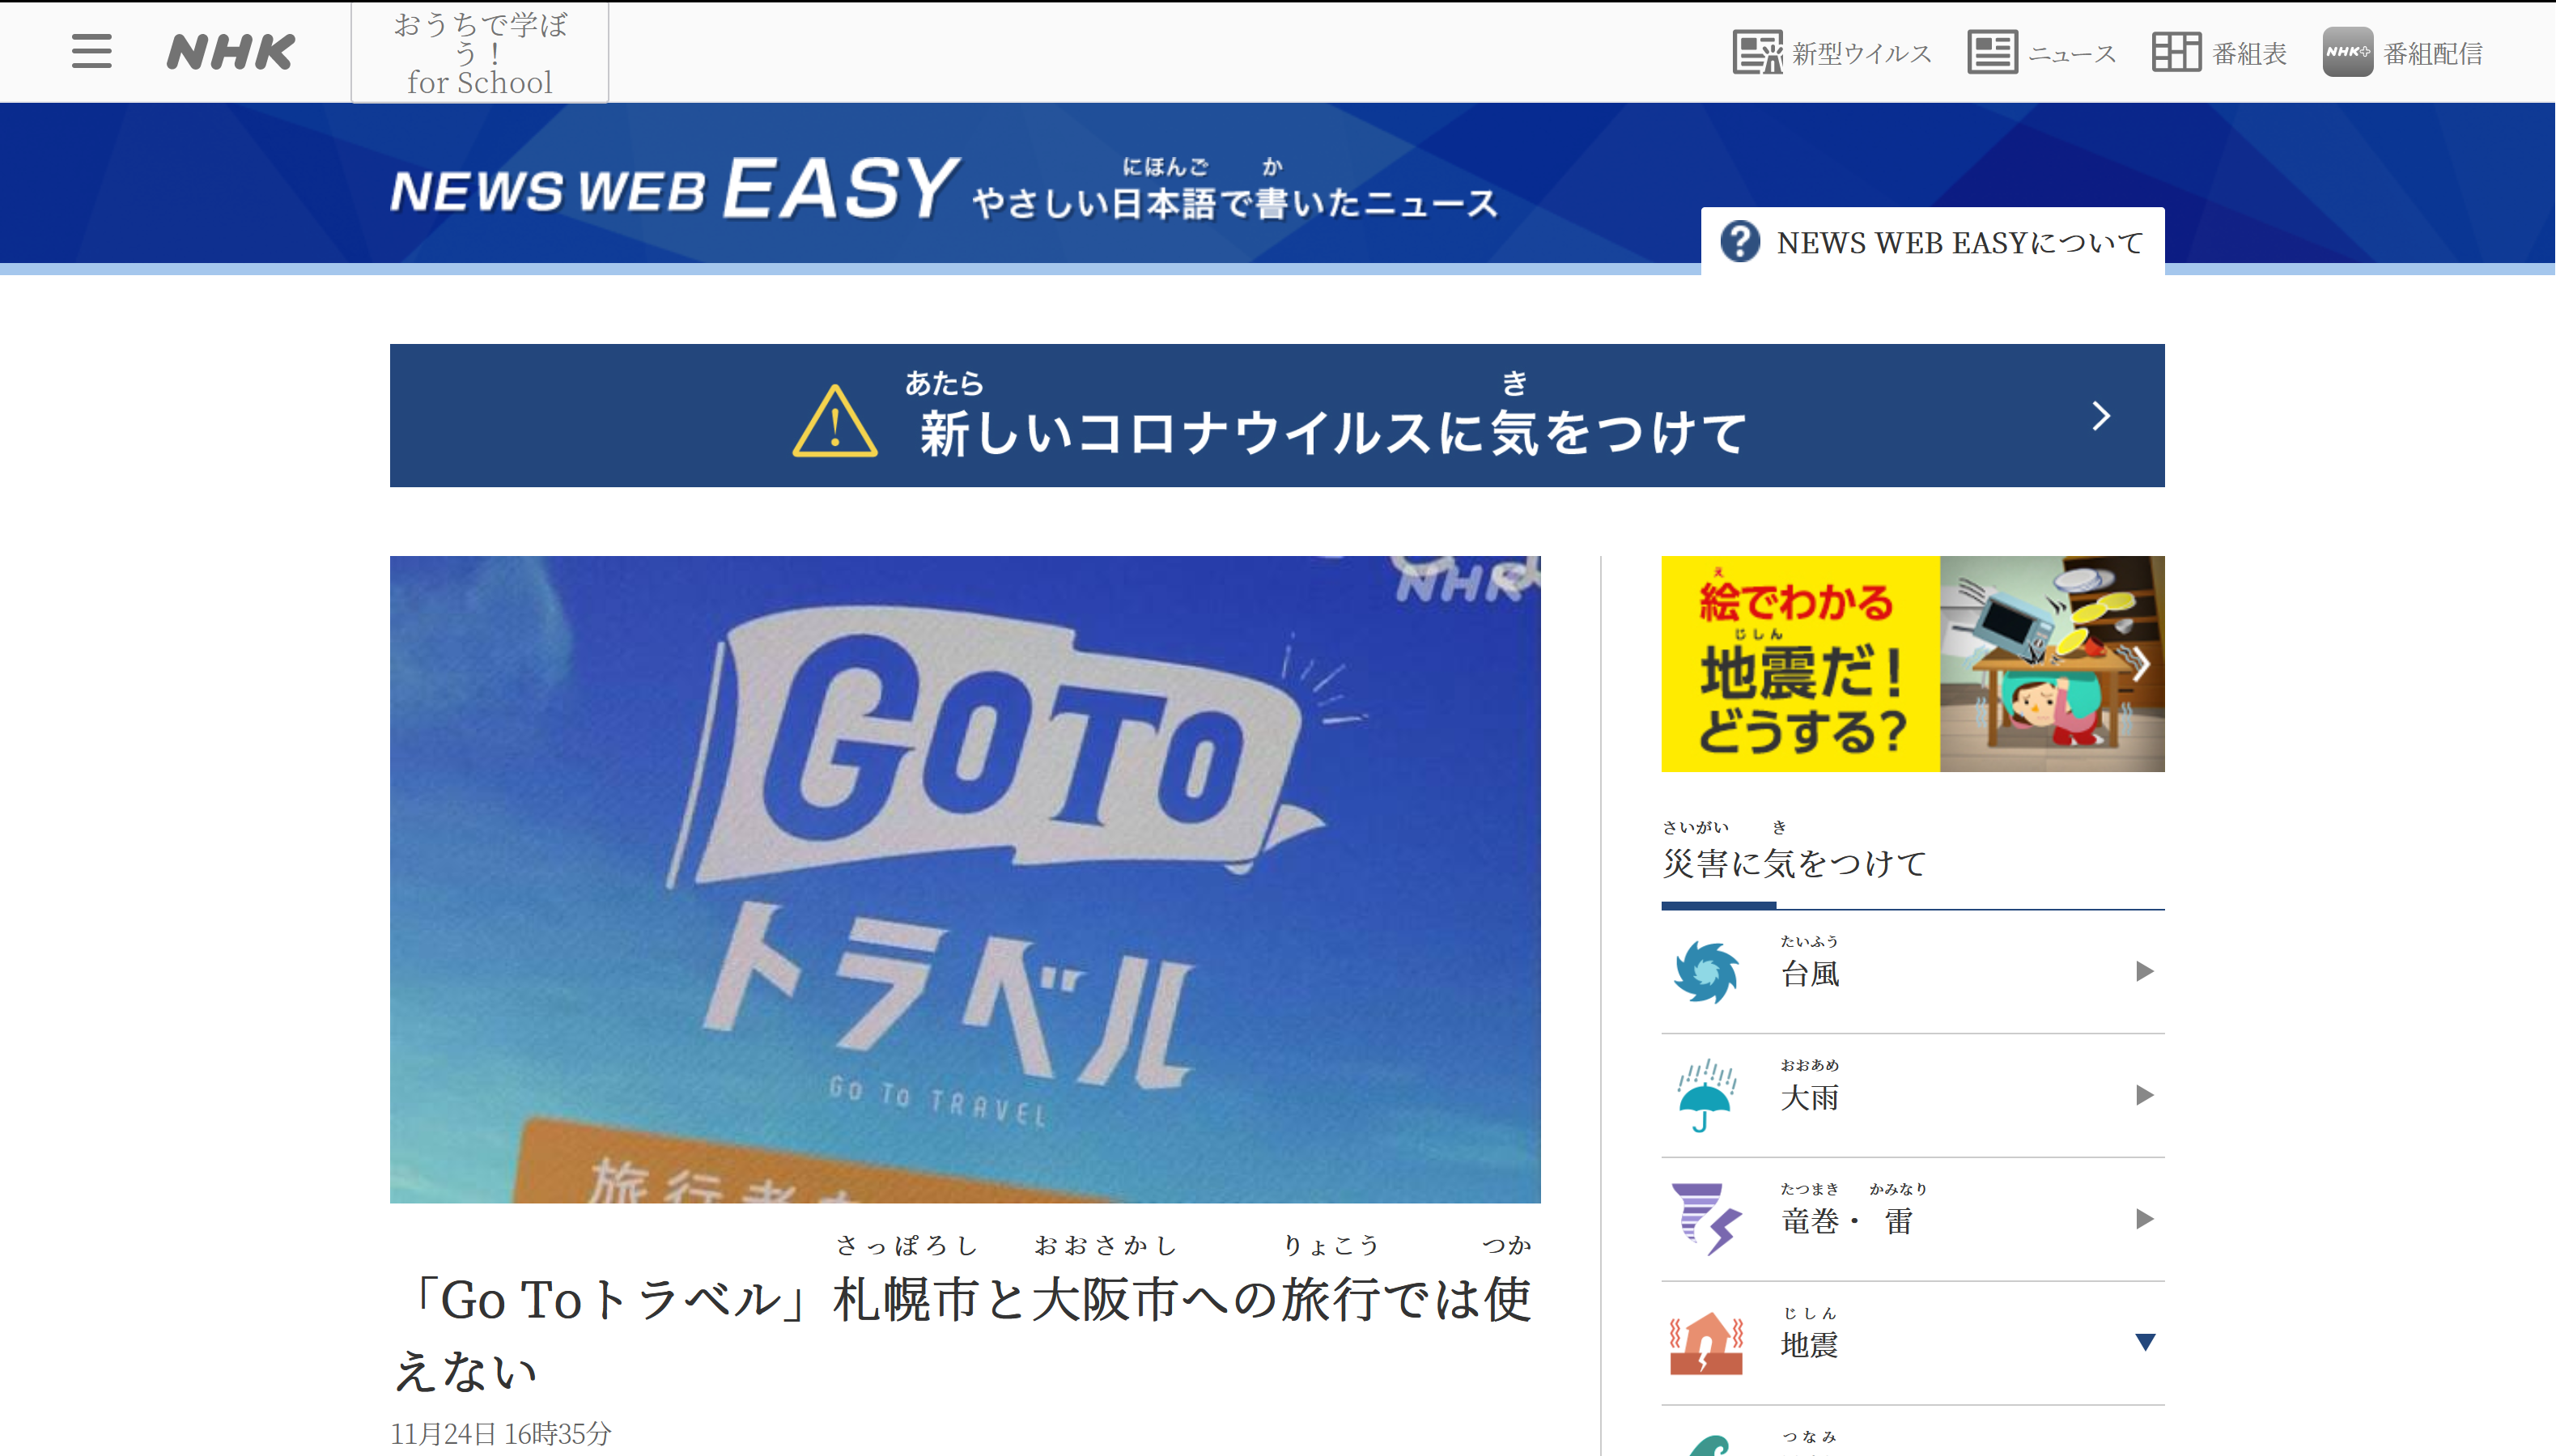
\includegraphics[width=\textwidth]{NHKniYoukoso.png}
  \caption{Главная страница News Web Easy}
  \label{NHK}
\end{figure}


%% ---------- subsection ---------- %%
\section{Текущее положение дел в системах упрощения текстов}
%% ---------- subsection ---------- %%


Вообще говоря, на сегодняшний пока ещё день не существует достаточно качественной системы упрощения текстов, способной заменить ручной перевод "--- дела здесь обстоят немногим лучше машинного перевода (из одного языка в другой), что можно объяснить отсутствием качественного и масштабного корпуса для обучения модели упрощения текстов (не только для японского языка, но даже для английского) и довольно высокой сложностью самой задачи, связанной с необходимостью «понимать» текст, что, к сожалению, современный искусственный интеллект сделать пока ещё не в состоянии.

Тем не менее, подобно тому, как сегодня используются системы машинного перевода (например, перевод отдельных слов или перевод текстов с последующими ручными корректировками), могут использоваться и системы упрощения текстов.
             % Глава 1
% \ContinueChapterBegin % размещать главы <<подряд>> 
%!TeX root = ../My_thesis.tex
\chapter{Название второй главы: разработка метода, алгоритма, модели исследования} \label{ch2}
	
% не рекомендуется использовать отдельную section <<введение>> после лета 2020 года
%\section{Введение} \label{ch2:intro}

Глава посвящена более подробным примерам оформления текстово-графических объектов.

В параграфе \ref{ch2:title-abbr} приведены примеры оформления многострочной формулы и одиночного рисунка. Параграф \ref{ch2:sec-abbr} раскрывает правила оформления перечислений и псевдокода. В параграфе \ref{ch2:sec-very-short-title} приведены примеры оформления сложносоставных рисунков, длинных таблиц, а также теоремоподобных окружений.


\section{Название параграфа} \label{ch2:title-abbr} %название по-русски



%%%%
%%		
%%  \input{...} commands are used only to sychronize some parts of the text with the author guide. Authors are free to type the text directly in .tex-files   
%%  \input{...} комманды используются только, чтобы синхронизировать части текта с рекомендациями авторам. Авторы  вольны вносить текст непосредственно в файл главы  
%%  
 %% ВНИМАНИЕ: для того, чтобы избежать лишнего отступа между текстом  и формулами, пожалуйста, начинайте формулы без пропуска строки в исходном коде как в строках #2 и #3.
	Все формулы, размещенные в отдельных строках, подлежат нумерации, например, как формулы \eqref{eq:UpArrow-G} и \eqref{eq:DownArrow-G} из \cite{Ganter1999}. 
	\begin{align}
	\label{eq:UpArrow-G}
	& A\uA =  \{ m\in{}M\:|\:gIm\:\forall  g \in{} A \}; \\ 
	\label{eq:DownArrow-G}
	& B\dA =  \{ g\in{}G\:|\:gIm\:\forall  m \in{} B \}.
	\end{align}

Обратим внимание, что формулы содержат знаки препинания и что они выровнены по левому краю (с помощью знака \verb|&| окружения \texttt{align}). % пример двух выравнивания двух формул в окружении align


На \firef{fig:spbpu-new-bld-autumn-ch2} приведёна фотография Нового научно-исследовательского корпуса СПбПУ.

	\begin{figure}[ht] 
	\center
	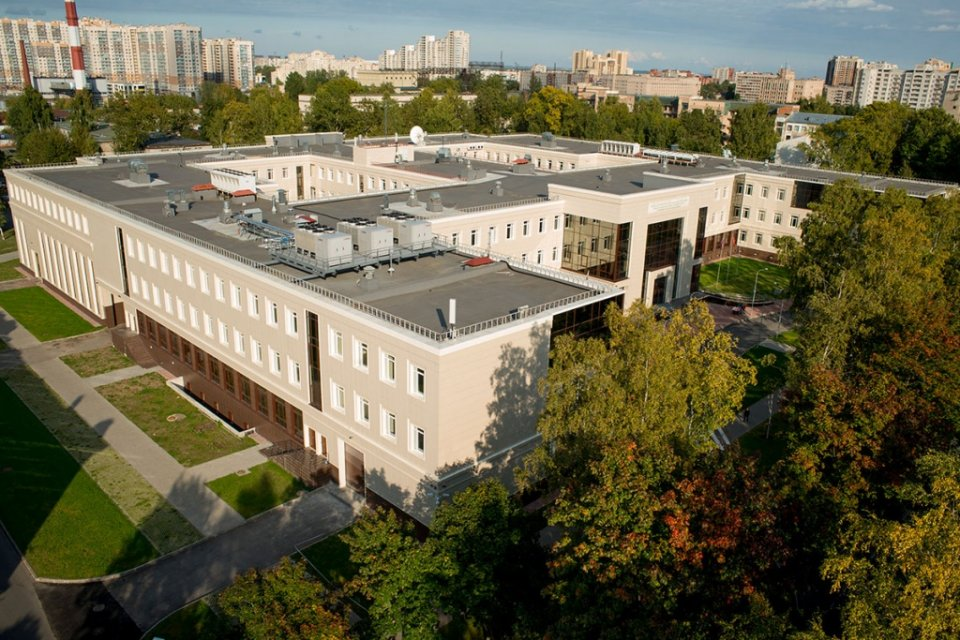
\includegraphics [scale=0.27] {my_folder/images/spbpu_new_bld_autumn}
	\caption{Новый научно-исследовательский корпус СПбПУ \cite{spbpu-gallery}} 
	\label{fig:spbpu-new-bld-autumn-ch2}  
	\end{figure}
	


	
\section{Название параграфа} \label{ch2:sec-abbr} %название по-русски
	
Название параграфа оформляется с помощью команды \verb|\section{...}|, название главы --- \verb|\chapter{...}|. 
	

\subsection{Название подпараграфа} \label{ch2:subsec-title-abbr} %название по-русски


Название подпараграфа оформляется с помощью команды  \texttt{\textbackslash{}subsection\{...\}}.


%\subsubsection{Название подподпараграфа} \label{ch2:subsubsec-title-abbr} %название по-русски
	
Использование подподпараграфов в основной части крайне не рекомендуется. В случае использования, необходимо вынести данный номер в содержание.	
Название подпараграфа оформляется с помощью команды  \texttt{\textbackslash{}subsubsecti\-on\{...\}}.



Вместо подподпараграфов рекомендовано использовать перечисления.

Перечисления могут быть с нумерационной частью и без неё и использоваться с иерархией и без иерархии. Нумерационная часть при этом формируется следующим способом:

\begin{enumerate}[1.]
	\item в перечислениях {\itshape без иерархии} оформляется арабскими цифрами с точкой (или длинным тире).
	\item В перечислениях {\itshape с иерархией} --- в последовательности сначала прописных латинских букв с точкой, затем арабских цифр с точкой и далее --- строчных латинских букв со скобкой. 
\end{enumerate}


%% Если в дальнейшем нужно сделать сслыку на один из элементов нумеруемого перечисления, то нужно использовать конктрукцию типа:

%\begin{enumerate}[label=\arabic{enumi}.,ref=\arabic{enumi}]
%	\item text 1 \label{item:text1}
%	\item text 2
%\end{enumerate}
%\ref{item:text1}.


Далее приведён пример перечислений с иерархией.


\begin{enumerate}
	\item Первый пункт.
	\item Второй пункт.
	\item Третий пункт.
	\item По ГОСТ 2.105--95 \cite{gost-russian-text-documents} первый уровень нумерации идёт буквами русского или латинского алфавитов ({\itshape для определенности выбираем английский алфавит}),
	а второй "--- цифрами. 
	\begin{enumerate}
		\item В данном пункте лежит следующий нумерованный список: 
		\begin{enumerate}
			\item первый пункт;
			\item третий уровень нумерации не нормирован ГОСТ 2.105--95 ({\itshape для определенности выбираем английский алфавит});
			\item обращаем внимание на строчность букв в этом нумерованном и следующем маркированном списке:
			\begin{itemize}
				\item первый пункт маркированного списка.
			\end{itemize}    
		\end{enumerate}
	\end{enumerate}
	\item Пятый пункт верхнего уровня перечисления.
\end{enumerate}

Маркированный список (без нумерационной части) используется, если нет необходимости ссылки на определенное положение в списке:
\begin{itemize}
	\item первый пункт c {\itshape маленькой буквы} по правилам русского языка;
	\item второй пункт c {\itshape маленькой буквы} по правилам русского языка.
\end{itemize} % правила использования перечислений	

	
Оформление псевдокода необходимо осуществлять с помощью пакета \verb|algorithm2e| в окружении \verb|algorithm|. Данное окружение интерпретируется в шаблоне как рисунок. Пример оформления псевдокода алгоритма приведён на \firef{alg:AlgoFDSCALING}. 
	
	
	\begin{algorithm} %[h]
		\SetKwFunction{algoDTestsFDSCALING}{} 
		\SetKwProg{myalg}{Algorithm}{}{} %write in 2nd agrument <<Algorithm>>, <<Procedure>> etc
		\nonl\myalg{\algoDTestsFDSCALING}{
			\KwInput{the many-valued context $\cont[M]\eqdef(G,M,W,J)$, the class membership $\epsilon: G\to K$} 
			\KwOutput{positive and negative binary contexts $\overbar{\cont[K]_+}\eqdef(\overbar{G_+},M,I_+)$, $\overbar{\cont[K]_-}\eqdef(\overbar{G_-},M,I_-)$ such that i-tests found in $\overbar{\cont[K]_+}$ are diagnostic tests in $\cont[M]$, and objects from $\overbar{\cont[K]_-}$ are counter-examples} %последние строки формируют начальное множество диагностических тестов
			\For {$\forall g_i,$ $g_j \in G$\label{step:FD-scaling-first-step}}{
				%(\tcp*[f]{possible inlined comment})
				\If{$i < j$ }{
					$\overbar{G} \leftarrow (g_i,g_j)$\;
				}
			}
			%		$M\leftarrow M\setminus k$\;
			\For {$\forall (g_i,g_j)\in \overbar{G}$}{
				%(\tcp*[f]{possible inlined comment})
				\If{$m(g_i) = m(g_j)$ }{ %на самом деле здесь цикл по всем компонентам вектора-строки
					$(g_i,g_j) I m$\; % or setI() function
				}
				\uIf{$\epsilon(g_i) = \epsilon(g_j)$ }{
					$\overbar{G_+} \leftarrow (g_i,g_j)$\;
				}
				\lElse{$\overbar{G_-} \leftarrow (g_i,g_j)$\label{FD-scaling-step-last}}	
			}		
			$I_+= I\cap (\overbar{G_+}\times M)$, $I_-= I\cap (\overbar{G_-}\times M)$\label{FD-scaling-step-newK}\; 
			\For {$\forall \overbar{g_+}\in \overbar{G_+}$, $\forall \overbar{g_-}\in \overbar{G_-}$ }{
				\If{$\overbar{g_+}\uA \subseteq \overbar{g_-}\uA$ }{
					$\overbar{G_+} \leftarrow \overbar{G_+} \setminus \overbar{g_+}$\;
				}
			}
			%		\Return \;
		}
		\caption{Псевдокод алгоритма \texttt{DiagnosticTestsScalingAndInferring} \cite{Naidenova2017}}\label{alg:AlgoFDSCALING}
		% example of adding an item to Index
		% \index for accepted papers only
		\index[ru]{алгоритм!\texttt{название\_алгоритма}} 
		% key words <<алгоритм>> и <<algorithm>> keep unmodified
		\index[en]{algorithm!\texttt{algorighm\_title}}
		% authors can used the key word <<процедура>> (procedure) и т.п.
		%
		%
	    % another example:
		\index[ru]{алгоритм!\texttt{DiagnosticTestsScaling\-AndInferring}} %нужен ручной перенос \- из-за ошибки в MakeIndex для команды \texttt
		%ключевые слова <<алгоритм>> и <<algorithm>> не менять
		\index[en]{algorithm!\texttt{DiagnosticTestsScaling\-AndInferring}} %нужен ручной перенос \- из-за ошибки в MakeIndex для команды \texttt
	\end{algorithm} 
	
	% another example of adding an arbitrary keyword to Index
	% some useful keywords: theorem, proposition, lemma, equation etc
	% please, use short keywords (2-3 max)
	\index[ru]{длинное-название-возможное-например-на-немецком} % длинные названия первого уровня как правило запрещены
	\index[en]{long-title-possible-for-example-in-German} 
	
Обратим внимание, что можно сослаться на строчку \ref{step:FD-scaling-first-step} псевдокода из \firef{alg:AlgoFDSCALING}.  % пример оформления псевдокода алгоритма 	

	
\section{Название параграфа} \label{ch2:sec-very-short-title} %название по-русски


	
%% ВНИМАНИЕ: для того, чтобы избежать лишнего отступа между текстом  и формулами, пожалуйста, начинайте формулы без пропуска строки в исходном коде как в строках #2 и #3.
Одиночные формулы также, как и отдельные формулы в составе группы, могут быть размещены в несколько строк. Чтобы выставить номер формулы напротив средней строки, используйте окружение \verb|multlined| из пакета \verb|mathtools| следующим образом \cite{Ganter1999}:
\begin{equation} % \tag{S} % tag - вписывает свой текст 
\label{eq:fConcept-order-G}
\begin{multlined}
(A_1,B_1)\leq (A_2,B_2)\; \Leftrightarrow \\  \Leftrightarrow\; A_1\subseteq A_2\; \Leftrightarrow \\ \Leftrightarrow\; B_2\subseteq B_1. 
\end{multlined}
\end{equation}

	
Используя команду \verb|\labelcref{...}| из пакета \verb|cleveref|, допустимо оформить ссылку на несколько формул, например, (\labelcref{eq:UpArrow-G,eq:DownArrow-G,eq:fConcept-order-G}). % пример оформления одиночной формулы в несколько строк

Пример оформления четырёх иллюстраций в одном текстово-графическом объекте приведён на \firef{fig:spbpu_sc-four-photos}. Это возможно благодаря использованию пакета \verb|subcaption|.

\begin{figure}[ht]
	\adjustbox{minipage=1.3em,valign=t}{\subcaption{}\label{fig:spbpu_sc-a}}%
	\begin{subfigure}[t]{\dimexpr.5\linewidth-1.3em\relax}
		\centering
		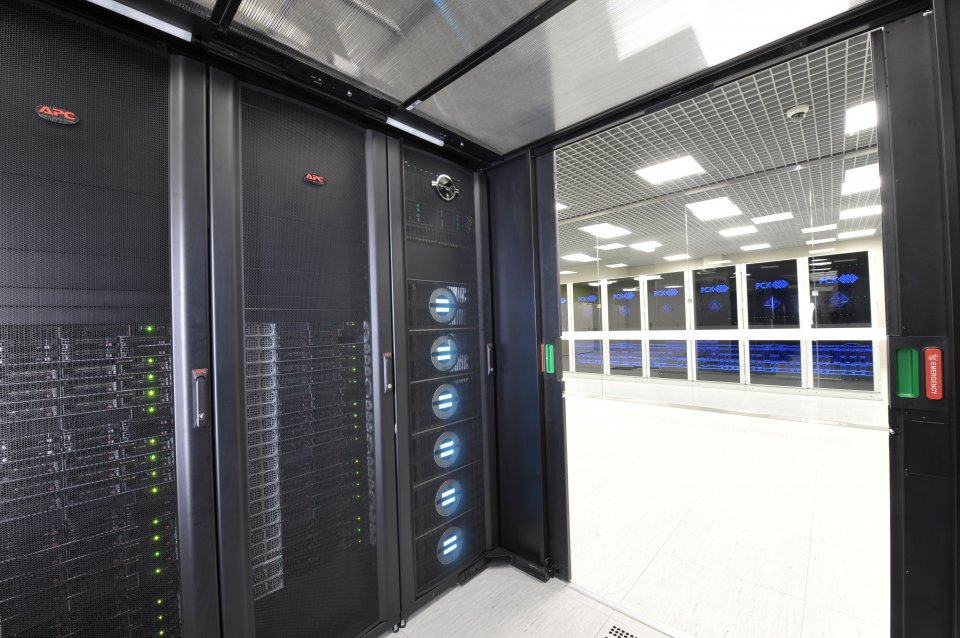
\includegraphics[width=.95\linewidth,valign=t]{my_folder/images/spbpu_sc_system}
	\end{subfigure}
\hfill %выровнять по ширине
	\adjustbox{minipage=1.3em,valign=t}{\subcaption{}\label{fig:spbpu_sc-b}}%
	\begin{subfigure}[t]{\dimexpr.5\linewidth-1.3em\relax}
		\centering
		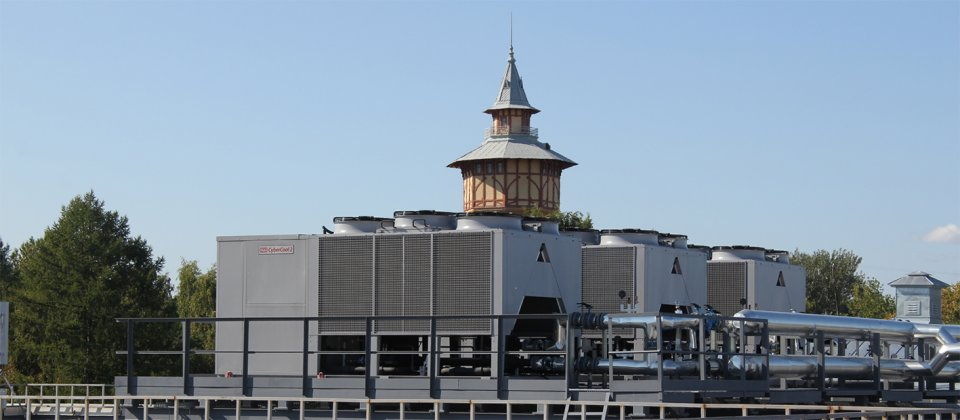
\includegraphics[width=.95\linewidth,valign=t]{my_folder/images/spbpu_sc_refr}
	\end{subfigure}
\\[20pt]
	\adjustbox{minipage=1.3em,valign=t}{\subcaption{}\label{fig:spbpu_sc-c}}%
\begin{subfigure}[t]{\dimexpr.5\linewidth-1.3em\relax}
	\centering
	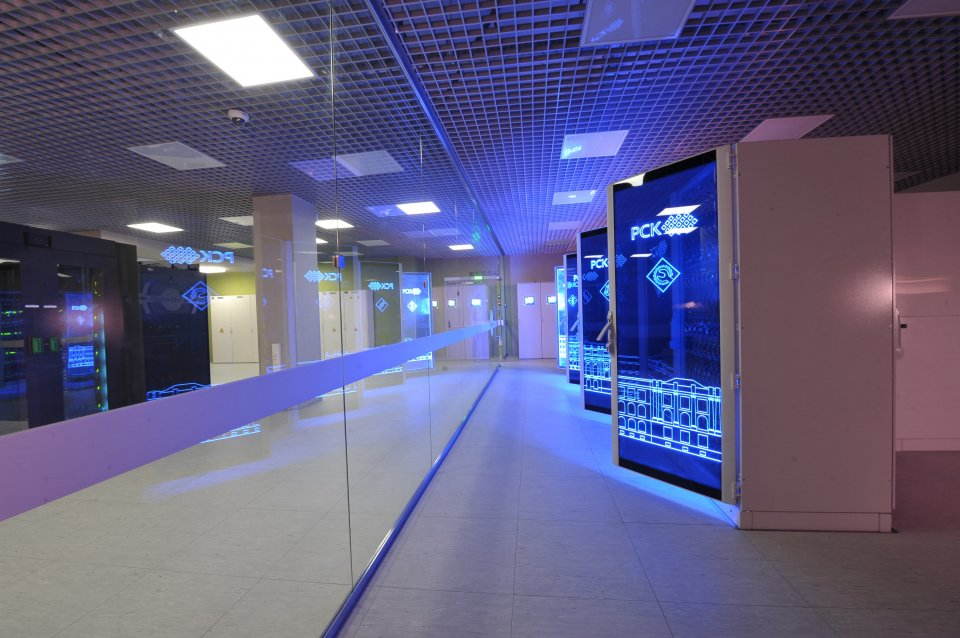
\includegraphics[width=.95\linewidth,valign=t]{my_folder/images/spbpu_sc_hall}
\end{subfigure}%
\hfill %выровнять по ширине
\adjustbox{minipage=1.3em,valign=t}{\subcaption{}\label{fig:spbpu_sc-d}}%
\begin{subfigure}[t]{\dimexpr.5\linewidth-1.3em\relax}
	\centering
	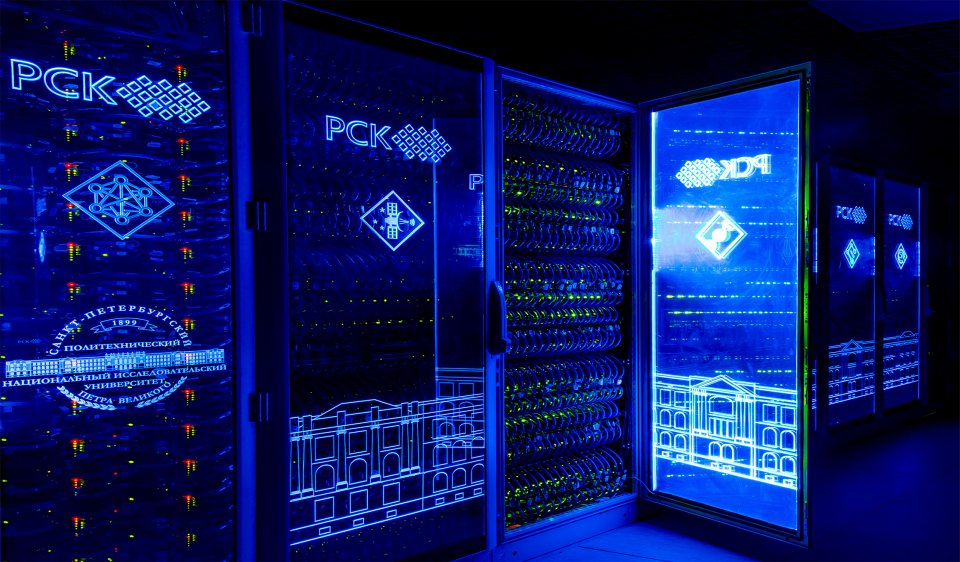
\includegraphics[width=.95\linewidth,valign=t]{my_folder/images/spbpu_sc_box}
\end{subfigure}
\captionsetup{justification=centering} %центрировать
\caption{Фотографии суперкомпьютерного центра СПбПУ \cite{spbpu-gallery}: {\itshape a} --- система хранения данных и узлы NUMA-вычислителя; {\itshape b} --- холодильные машины на крыше научно-исследовательского корпуса; {\itshape c} --- машинный зал; {\itshape d} --- элементы вычислительных устройств} 
\label{fig:spbpu_sc-four-photos}
\end{figure}

Далее можно ссылаться на составные части данного рисунка как на самостоятельные объекты: \firef{fig:spbpu_sc-a}, \firef{fig:spbpu_sc-b}, \firef{fig:spbpu_sc-c}, \firef{fig:spbpu_sc-d} или на три из четырёх изображений одновременно: рис.\labelcref{fig:spbpu_sc-a,fig:spbpu_sc-b,fig:spbpu_sc-c}. % пример подключения 4х иллюстраций в одном рисунке

%На \firef{fig:spbpu_whitehall-three-photos} приведены три картинки под~общим номером и~названием, но с раздельной нумерацией подрисунков посредством пакета \verb|subcaption|.
%
\begin{figure}[!htbp]
	\adjustbox{minipage=1.3em,valign=t}{\subcaption{}\label{fig:spbpu_whitehall-a}}%
	\begin{subfigure}[t]{\dimexpr.3\linewidth-1.3em\relax}
		\centering
		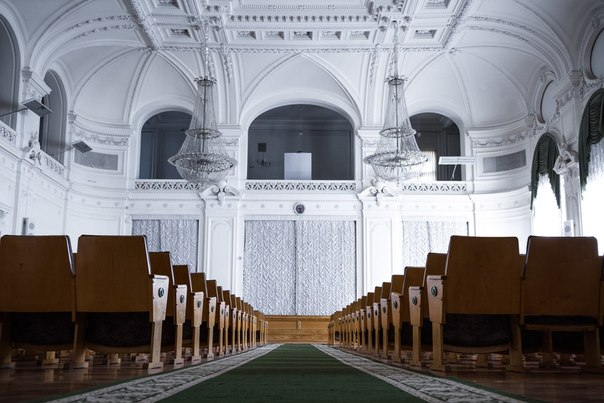
\includegraphics[width=.95\linewidth,valign=t]{my_folder/images//spbpu_whitehall}
	\end{subfigure}
	\hfill %выровнять
	\adjustbox{minipage=1.3em,valign=t}{\subcaption{}\label{fig:spbpu_whitehall-b}}%
	\begin{subfigure}[t]{\dimexpr.3\linewidth-1.3em\relax}
		\centering
		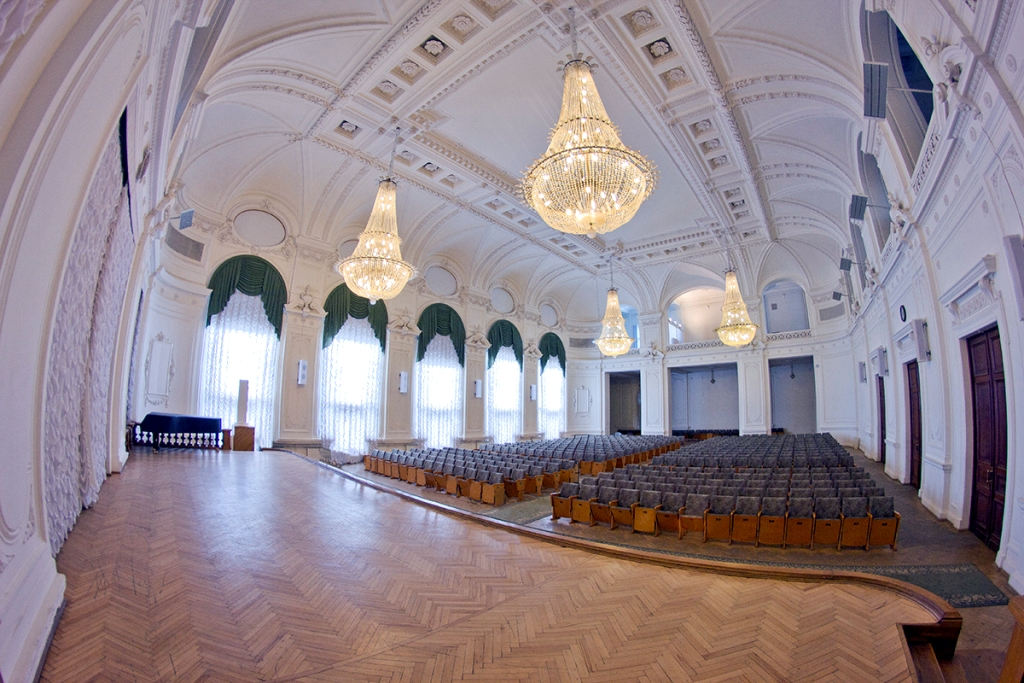
\includegraphics[width=.95\linewidth,valign=t]{my_folder/images//spbpu_whitehall_ligh}
	\end{subfigure}
	\hfill %выровнять
		\adjustbox{minipage=1.3em,valign=t}{\subcaption{}\label{fig:spbpu_whitehall-c}}%
	\begin{subfigure}[t]{\dimexpr.3\linewidth-1.3em\relax}
		\centering
		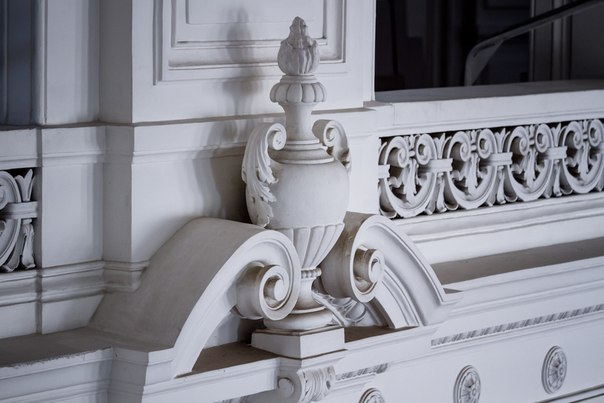
\includegraphics[width=.95\linewidth,valign=t]{my_folder/images//spbpu_whitehall_sculpture}
	\end{subfigure}%
\captionsetup{justification=centering} %центрировать
	\caption{Фотографии Белого зала СПбПУ \cite{spbpu-gallery}, в том числе: {\itshape a} --- со стороны зрителей; {\itshape b} --- со стороны сцены; {\itshape c} --- барельеф}\label{fig:spbpu_whitehall-three-photos}  
\end{figure}

Далее можно ссылаться на три отдельных рисунка: \firef{fig:spbpu_whitehall-a}, \firef{fig:spbpu_whitehall-b} и \firef{fig:spbpu_whitehall-c}. % пример подключения 3х иллюстрации в одном рисунке
%
%На \firef{fig:spbpu_main_bld-two-photos} приведены две картинки под~общим номером и~названием.


\begin{figure}[!htbp]
	\adjustbox{minipage=1.3em,valign=t}{\subcaption{}\label{fig:spbpu_main_bld_entrance_autumn}}%
	\begin{subfigure}[t]{\dimexpr.5\linewidth-1.3em\relax} %разрешили выделить 0,5 стр в ширину на рисунок
		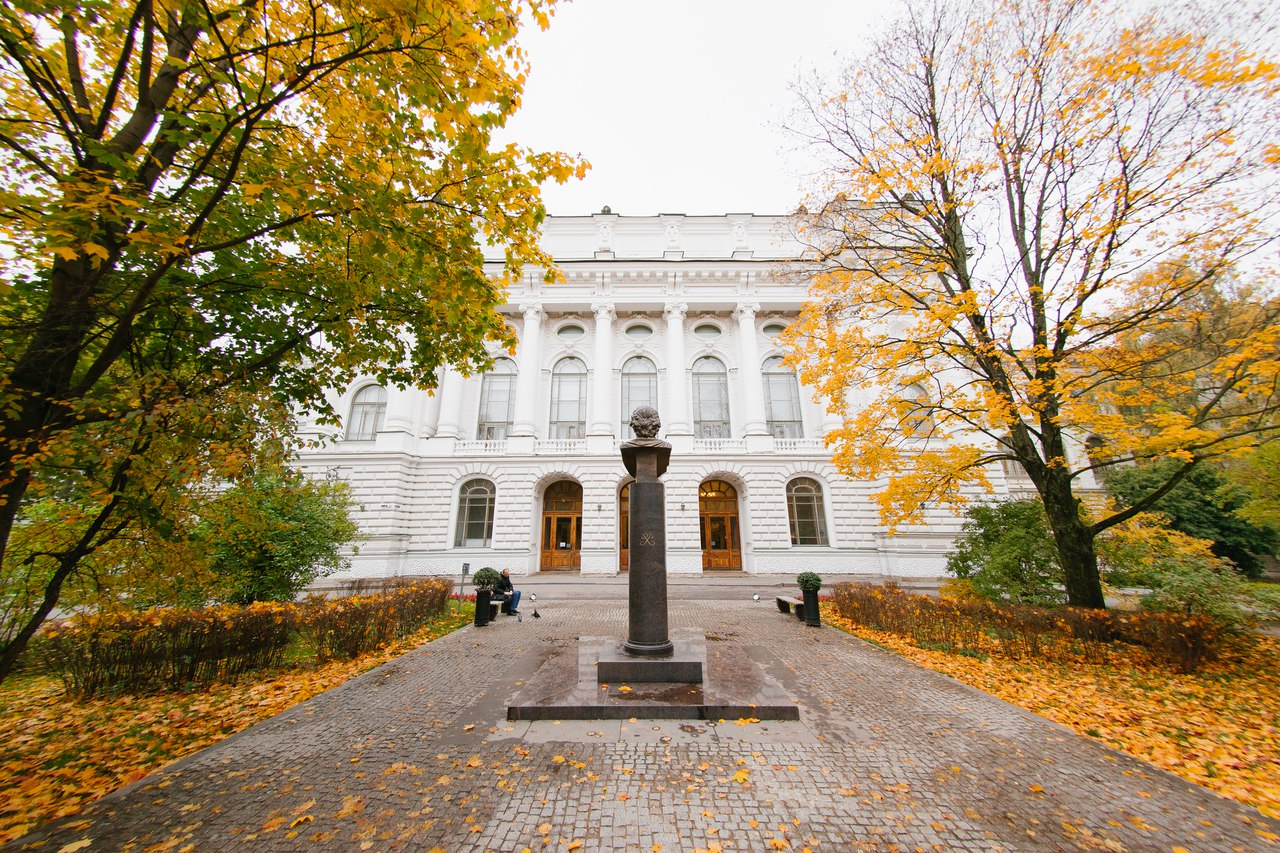
\includegraphics[height=0.20\textheight,valign=t]{my_folder/images//spbpu_main_bld_entrance_autumn} %высоту рисунка выставили как 0,3 от высоты наборного поля
	\end{subfigure}
%	\hfill %выровнять по ширине
	\adjustbox{minipage=1.3em,valign=t}{\subcaption{}\label{fig:spbpu_main_bld_whitehall}}%
	\begin{subfigure}[t]{\dimexpr.5\linewidth-1.3em\relax}%разрешили выделить 0,5 стр в ширину на рисунок
		
\includegraphics[height=0.20\textheight,valign=t]{my_folder/images//spbpu_main_bld_whitehall}%высоту рисунка выставили как 0,3 от высоты наборного поля
	\end{subfigure}
\captionsetup{justification=centering} %центрировать
	\caption{Вид на главное здание СПбПУ \cite{spbpu-gallery}, включая: {\itshape a} --- вход со стороны парка осенью; {\itshape b}~--- окна Белого зала}\label{fig:spbpu_main_bld-two-photos} 
\end{figure}

На \firef{fig:spbpu_main_bld_entrance_autumn} изображен вход со стороны парка СПбПУ осенью, а на \firef{fig:spbpu_main_bld_whitehall}~--- окна Белого зала. % пример подключения 2х иллюстраций в одном рисунке

Приведём пример табличного представления данных с записью продолжения на следующей странице на \taref{tab:long}.

%%% отладка longtable
%% 1) для контроля выхода таблицы за границы полей выставляем showframe в \geometry{}, см настройки
%% 2) используем \\* для запрета переноса определенной строки или средства из:
%% https://tex.stackexchange.com/q/344270/44348
%% 3) в крайнем случае для принудительного переноса таблицы на новую страницу используем \pagebreak после \\
\noindent % for correct centering
\begingroup
\centering
\small %выставляем шрифт в 12bp
\begin{longtable}[c]{|l|l|l|l|l|l|}
	\caption{Пример задания данных из \cite{Peskov2004} (с повтором для переноса таблицы на новую страницу)}%
	\label{tab:long}% label всегда желательно идти после caption
	\\
	\hline
	$G$&$m_1$&$m_2$&$m_3$&$m_4$&$K$\\ \hline
	1&2&3&4&5&6\\ \hline
	\endfirsthead%
	\captionsetup{format=tablenocaption,labelformat=continued} % до caption!
	\caption[]{}\\ % печать слов о продолжении таблицы
	\hline
	1&2&3&4&5&6\\ \hline
	\endhead
	\hline
	\endfoot
	\hline
	\endlastfoot
	$g_1$&0&1&1&0&1\\ \hline
	$g_2$&1&2&0&1&1\\ \hline
	$g_3$&0&1&0&1&1\\ \hline
	$g_4$&1&2&1&0&2\\ \hline
	$g_5$&1&1&0&1&2\\ \hline
	$g_6$&1&1&1&2&2\\ \hline
%
	$g_1$&0&1&1&0&1\\ \hline 
	$g_2$&1&2&0&1&1\\ \hline
	$g_3$&0&1&0&1&1\\ \hline
	$g_4$&1&2&1&0&2\\ \hline \noalign{\penalty-5000} % способствуем переносу на следующую стр
	$g_5$&1&1&0&1&2\\ \hline 
	$g_6$&1&1&1&2&2\\ \hline
%
	$g_1$&0&1&1&0&1\\ \hline 
	$g_2$&1&2&0&1&1\\ \hline
	$g_3$&0&1&0&1&1\\ \hline
	$g_4$&1&2&1&0&2\\ \hline
	$g_5$&1&1&0&1&2\\ \hline
	$g_6$&1&1&1&2&2\\ \hline
%		
	$g_1$&0&1&1&0&1\\ \hline 
	$g_2$&1&2&0&1&1\\ \hline
	$g_3$&0&1&0&1&1\\ \hline
	$g_4$&1&2&1&0&2\\ \hline
	$g_5$&1&1&0&1&2\\ \hline
	$g_6$&1&1&1&2&2\\ \hline
%
	$g_1$&0&1&1&0&1\\ \hline 
	$g_2$&1&2&0&1&1\\ \hline
	$g_3$&0&1&0&1&1\\ \hline
	$g_4$&1&2&1&0&2\\ \hline
	$g_5$&1&1&0&1&2\\ \hline
	$g_6$&1&1&1&2&2\\ \hline
%
	$g_1$&0&1&1&0&1\\ \hline 
	$g_2$&1&2&0&1&1\\ \hline
	$g_3$&0&1&0&1&1\\ \hline
	$g_4$&1&2&1&0&2\\ \hline
	$g_5$&1&1&0&1&2\\ \hline
	$g_6$&1&1&1&2&2\\ \hline
%
	$g_1$&0&1&1&0&1\\ \hline 
	$g_2$&1&2&0&1&1\\ \hline
	$g_3$&0&1&0&1&1\\ \hline
	$g_4$&1&2&1&0&2\\ \hline
	$g_5$&1&1&0&1&2\\ \hline
	$g_6$&1&1&1&2&2\\ \hline
\end{longtable}
\normalsize% возвращаем шрифт к нормальному
\endgroup % пример подключения таблицы на несколько страциц


\begin{table} [htbp]% Пример оформления таблицы
	\centering\small
	\caption{Пример представления данных для сквозного примера по ВКР \cite{Peskov2004}}%
	\label{tab:ToyCompare}		
		\begin{tabular}{|l|l|l|l|l|l|}
			\hline
			$G$&$m_1$&$m_2$&$m_3$&$m_4$&$K$\\
			\hline
			$g_1$&0&1&1&0&1\\ \hline
			$g_2$&1&2&0&1&1\\ \hline
			$g_3$&0&1&0&1&1\\ \hline
			$g_4$&1&2&1&0&2\\ \hline
			$g_5$&1&1&0&1&2\\ \hline
			$g_6$&1&1&1&2&2\\ \hline		
		\end{tabular}
%	\caption*{\raggedright\hspace*{2.5em} Составлено (или/и рассчитано) по \cite{Peskov2004}} %Если проведена авторская обработка или расчеты по какому-либо источнику	
	\normalsize% возвращаем шрифт к нормальному
\end{table}



%% please, before using, read the author guide carefully

\noindent % for correct centering
\begin{minipage}{\textwidth}
	\vspace{\mfloatsep} % интервал 
	\centering\small
	\captionof{table}{Пример задания данных в табличном виде из \cite{Peskov2004} (с помощью окружения minipage)}%
	\label{tab:ToyCompare-Peskov-minipage}
	\begin{tabular}{|l|l|l|l|l|l|}
	\hline
	$G$&$m_1$&$m_2$&$m_3$&$m_4$&$K$\\
	\hline
	$g_1$&0&1&1&0&1\\ \hline
	$g_2$&1&2&0&1&1\\ \hline
	$g_3$&0&1&0&1&1\\ \hline
	$g_4$&1&2&1&0&2\\ \hline
	$g_5$&1&1&0&1&2\\ \hline
	$g_6$&1&1&1&2&2\\ \hline
	\hline		
	\end{tabular}
\vspace{\mfloatsep} % интервал 
\normalsize %восстанавливаем шрифт 	
\end{minipage} % пример подключения minipage

\noindent % for correct centering
\begin{minipage}{\textwidth}
	\centering
	\vspace{\mfloatsep} % интервал  	
	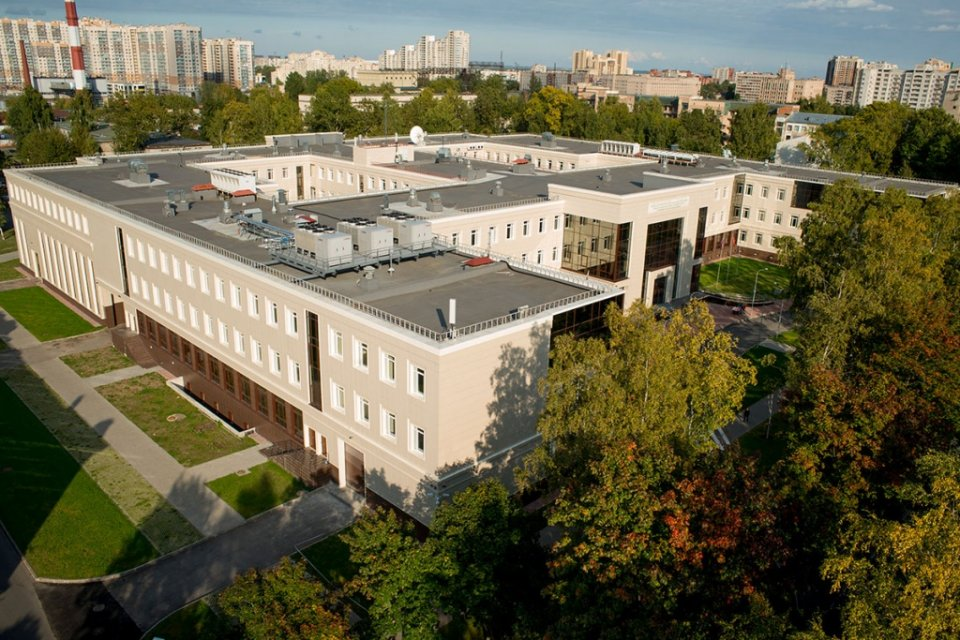
\includegraphics[keepaspectratio=true,scale=0.27] {my_folder/images/spbpu_new_bld_autumn}
	\captionof{figure}{Новый научно-исследовательский корпус СПбПУ \cite{spbpu-gallery} (с помощью окружения minipage)}\label{fig:spbpu-new-bld-autumn-minipage}  
	\vspace{\mfloatsep} % интервал  	
\end{minipage} % пример подключения minipage




Вопросы форматирования текстово-графических объектов (окружений) не регламентированы в известных нам ГОСТах, поэтому предлагаем придерживаться следующих правил:

\begin{itemize}
	\item \textbf{полужирный текст} рекомендуем использовать только для названий стандартных окружений с нумерационной частью, например, для представления \textit{впервые}: \textbf{определение 1.1}, \textbf{теорема 2.2}, \textbf{пример 2.3}, \textbf{лемма 4.5};
	
	\item \textit{курсив} рекомендуем использовать только для выделения переменных в формулах, служебной информации об авторах главы (статьи), важных терминов, представляемых по тексту, а также для всего тела окружений, связанных с получением \textit{новых существенных результатов и их доказательством}: теорема, лемма, следствие, утверждение и другие.
\end{itemize}

 

По аналогии с нумерацией формул, рисунков и таблиц нумеруются и иные текстово-графические объекты, то есть включаем в нумерацию номер главы, например: теорема 3.1. для первой теоремы третьей главы монографии. Команды \LaTeX{} выставляют нумерацию и форматирование автоматически. Полный перечень команд для подготовки текстово-графических и иных объектов находится в подробных методических рекомендациях \cite{spbpu-bci-template-author-guide}. 


Для удобства авторов названия стандартных окружений, рекомендованных к использованию, приведены в \taref{tab:enum-std}, а в \taref{tab:enum-spbpu}  перечислены имена специально разработанных окружений для шаблонов SPbPU.

% и примеры их оформления на псевдокоде (см. \cite{cite-spbpu-bci}).


%https://tex.stackexchange.com/questions/2651/should-i-use-center-or-centering-for-figures-and-tables


	\begin{table} [htbp]% Пример записи таблицы с номером, но без отображаемого наименования
	\centering\small
	\caption{Стандартные окружения}%
	\label{tab:enum-std}
	 \begin{Spacing}{\Single} % Одинарный интервал между строками текста 
	  \renewcommand*{\arraystretch}{1.5} % Полуторный интервал между ячейками таблицы
		\begin{tabular}{|l|p{11cm}|} 
			\hline
			Название окружения&Назначение\\
			\hline
			\verb|center| &	центрирование, аналог команды \verb|\centering|, но с добавлением нежелательного пробела, поэтому лучше избегать применения \verb|center|\\ \hline
			\verb|itemize| &{перечисления, в которых нет необходимости нумеровать  пункты (немаркированные списки)} \\ \hline
			\verb|enumerate| & перечисления с нумерацией (немаркированные списки) \\ \hline
			\verb|refsection| & создание отдельных библиографических списков для глав \\ \hline
			\verb|tabular| & оформление таблиц \\ \hline
			\verb|table|   &{автоматическое перемещение по тексту таблиц, оформленных, например, с помощью \verb|tabular|, для минимизации пустых пространств} \\ \hline
			\verb|longtable| & оформление многостраничных таблиц \\ \hline
			\verb|tikzpicture| & создание иллюстраций с помощью пакета \verb|tikz| \cite{ctan-tikz} \\ \hline
			\verb|figure| &{автоматическое перемещение по тексту рисунков, оформленных например, с помощью \verb|tikz| или подключенных с помощью команды \verb|\includegraphics|, для минимизации пустых пространств} \\ \hline 
			\verb|subfigure| & оформление вложенных рисунков в составе \verb|figure| \\ \hline
			\verb|algorithm| &{оформление псевдокода на основе пакета \verb|algorithm2e| \cite{ctan-algorithm2e}} \\ \hline
			\verb|minipage| & {оформление рисунков и таблиц без функций автоматического перемещения по тексту для  минимизации пустых пространств} \\ \hline
			\verb|equation| & {оформление выключенных (не встроенных в текст с помощью \verb|$...$|) одиночных формул на одной строке} \\ \hline
			\verb|multilined| &{оформление выключенных (не встроенных в текст с помощью \verb|$...$|) одиночных формул в несколько строк} \\ \hline 
			\verb|aligned| &{оформление нескольких формул с выравниванием по символу \verb|&|.} \\ \hline
	\end{tabular}
	\end{Spacing}
%	\normalsize
	\end{table}

На базе пакета \verb|tikz| разработано большое количество расширений \cite{ctan-tikz}, например, \verb|tikzcd|, которые мы рекомендуем использовать для оформления иллюстраций.

	\begin{table} [htbp]% Пример записи таблицы с номером, но без отображаемого наименования
	\centering\small
	\caption{Специальные окружения}%
	\label{tab:enum-spbpu}
		\begin{tabular}{|l|l|}
			\hline
			Название окружения & Текстово-графический объект\\
			\hline
			\verb|abstr|	 & реферат (abstract) \\ \hline
			\verb|m-theorem| & теорема \\ \hline 
			\verb|m-corollary| & следствие \\ \hline
			\verb|m-proposition| & утверждение \\ \hline
			\verb|m-lemma|   & лемма \\ \hline
			\verb|m-axiom| & аксиома \\ \hline
			\verb|m-example| & пример \\ \hline
			\verb|m-definition| &  определение \\ \hline
			\verb|m-condition| & условие \\ \hline
			\verb|m-problem| & проблема \\ \hline
			\verb|m-exercise| & упраженение \\ \hline
			\verb|m-question| & вопрос \\ \hline
			\verb|m-hypothesis| & гипотеза \\ \hline
		\end{tabular}	
	\normalsize
\end{table}

В случае, если авторам потребовалось новое окружение, то создать его можно в файле в файле \texttt{my\_fol\-der/{}my\_set\-tings.tex} согласно правилам, приведённым ниже.

\begin{enumerate}[1.]
	\item Для перехода в режим создания окружений следует указать:
	\begin{itemize}
		\item \verb|\theoremstyle{myplain}| --- окружения с доказательствами или аксиомами
		\item \verb|\theoremstyle{mydefinition}| --- окружения, не связанные с доказательствами или аксиомами.
	\end{itemize}
	\item В команде создания окружения следует ввести краткий псевдоним (\verb|m-new-env|) и отображаемое в pdf имя окружения (\verb|Название_окружения|):
	\begin{itemize}
		\item \texttt{\textbackslash{}newtheorem\{m-new-env-second\}\{Название\_окруже\-ния\}\-[chap\-ter]}.
	\end{itemize}
\end{enumerate}


%\begin{m-new-env-first}
%	Тест первого пользовательского окружения
%\end{m-new-env-first}
%
%\begin{m-new-env-second}
%	Тест второго пользовательского окружения
%\end{m-new-env-second} % список некоторых окружений


\begin{m-theorem}[о чем-то конкретном] %при необходимости в [] можно записать название теоремы или убрать его
	\label{th:ex} 
	% \index только для принятых работ
	% шаблон записи теоремы в Предметный указатель
	\index[ru]{теорема!название\_теоремы или о чём} %ключевое слово <<теорема>> не менять
	\index[en]{theorem!1-3 words for detail or description}
	% пример записи алгоритма в Предметный указатель
	\index[ru]{теорема!о неполноте}
	\index[en]{theorem!about incompleteness}
	% пример записи алгоритма в Предметный указатель
	\index[ru]{теорема!о жизни}
	\index[en]{theorem!about life}
	Текст теоремы полностью выделен курсивом. Допустимо математические символы не выделять курсивом, если это искажает их значения. Используется абзацный отсуп, так как ``Абзацы в тексте начинают отступом'' в соответствии с ГОСТ 2.105--95. Название теоремы допустимо убрать. Доказательство окончено.
\end{m-theorem}
Доказательство теоремы \ref{th:ex}, леммы, утверждений, следствий и других подобных окружений (в последнем абзаце) завершаем предложением в котором сказано, что доказательство окончено. Например, доказательство теоремы \ref{th:ex} окончено.

Тело доказательства не выделяется курсивом.
Тело следующих окружений также не выделяется сплошным курсивом: определение, условие, проблема, пример, упражнение, вопрос, гипотеза и другие. %пример оформления теоремы


\begin{m-definition}[термин] %при необходимости в [] можно записать название определения или убрать его
	\label{def:ex}
	% \index только для принятых работ
	% шаблон записи определения в Предметный указатель 
	\index[ru]{название\_определения!1-3 уточняющих слова или~ничего}
	\index[en]{definition\_title!1-3 words for detail or~without "!-part}
	% пример записи определения в Предметный указатель 
	\index[ru]{и-тест!хороший!наилучший}
	\index[en]{i-test!good!best}
	% пример записи определения в Предметный указатель 
	\index[ru]{и-тест!замкнутый}
	\index[en]{i-test!closed}
	В тексте определения только {\itshape важные термины} выделяются курсивом. Если определение носит лишь вспомогательный характер, то допустимо не использовать окружение \texttt{m-definition}, представляя текст определения в обычном абзаце. Ключевые термины при этом обязательно выделяются курсивом.
\end{m-definition} %пример оформления определения


Вместо теоремо-подобных окружений для вставки небольших текстово-графических объектов иногда используются команды. Типичным примером такого подхода является команда \verb|\footnote{text}|\footnote{Внимание! Команда вставляется непосредственно после слова, куда вставляется сноска (без пробела). Лишние пробелы также не указываются внутри команды перед и после фигурных скобок.}, где в аргументе \verb|text| указывают текст \textit{подстрочной ссылки (сноски)}.В них \textit{нельзя добавлять веб-ссылки или цитировать литературу}. Для этих целей используется список литературы. Нумерация сносок сквозная по ВКР без точки на конце выставляется в шаблоне автоматически, однако в каждом приложении к ВКР нумерация, зависящая от номера приложения, выставляется префикс <<П>>, например <<П1.1>> --- первая сноска первого приложения. 




%\FloatBarrier % заставить рисунки и другие подвижные (float) элементы остановиться


\section{Выводы} \label{ch2:conclusion}

Текст заключения ко второй главе. Пример ссылок \cite{Article,Book,Booklet,Conference,Inbook,Incollection,Manual,Mastersthesis,Misc,Phdthesis,Proceedings,Techreport,Unpublished,badiou:briefings}, а также ссылок с указанием страниц, на котором отображены те или иные текстово-графические объекты  \cite[с.~96]{Naidenova2017} или в виде мультицитаты на несколько источников \cites[с.~96]{Naidenova2017}[с.~46]{Ganter1999}. Часть библиографических записей носит иллюстративный характер и не имеет отношения к реальной литературе. 

Короткое имя каждого библиографического источника содержится в специальном файле \verb|my_biblio.bib|, расположенном в папке \verb|my_folder|. Там же находятся исходные данные, которые с помощью программы \texttt{Biber} и стилевого файла \texttt{Biblatex-GOST} \cite{ctan-biblatex-gost} приведены в списке использованных источников согласно ГОСТ 7.0.5-2008.
Многообразные реальные примеры исходных библиографических данных можно посмотреть по ссылке \cite{ctan-biblatex-gost-examples}.

Как правило, ВКР должна состоять из четырех глав. Оставшиеся главы можно создать по образцу первых двух и подключить с помощью команды \verb|\input| к исходному коду ВКР. Далее в приложении \ref{appendix-MikTeX-TexStudio} приведены краткие инструкции запуска исходного кода ВКР \cite{latex-miktex,latex-texstudio}.

В приложении \ref{appendix-extra-examples} приведено подключение некоторых текстово-графических объектов. Они оформляются по приведенным ранее правилам. В качестве номера структурного элемента вместо номера главы используется <<П>> с номером главы. Текстово-графические объекты из приложений не учитываются в реферате.



%% Вспомогательные команды - Additional commands
%
%\newpage % принудительное начало с новой страницы, использовать только в конце раздела
%\clearpage % осуществляется пакетом <<placeins>> в пределах секций
%\newpage\leavevmode\thispagestyle{empty}\newpage % 100 % начало новой страницы             % Глава 2
%!TeX root = ../My_thesis.tex


% @inproceedings{my-dataset,
%     title = "Crowdsourced Corpus of Sentence Simplification with Core Vocabulary",
%     author = "Katsuta, Akihiro  and
%       Yamamoto, Kazuhide",
%     booktitle = "Proceedings of the Eleventh International Conference on Language Resources and Evaluation ({LREC} 2018)",
%     month = may,
%     year = "2018",
%     address = "Miyazaki, Japan",
%     publisher = "European Language Resources Association (ELRA)",
%     url = "https://www.aclweb.org/anthology/L18-1072",
% }


% .---|||___|||--- C H A P T E R ---|||___|||---. %
\chapter{Детали практической реализации}
% .---|||___|||--- C H A P T E R ---|||___|||---. %


% .---|||___|||--- S E C T I O N ---|||___|||---. %
\section{Инструменты и исходный код}
% .---|||___|||--- S E C T I O N ---|||___|||---. %


% .---|||___|||--- S U B S E C T I O N ---|||___|||---. %
\subsection{Выбор инструментов для системы упрощения}
% .---|||___|||--- S U B S E C T I O N ---|||___|||---. %


В данной работе используются следующие инструменты:
\begin{enumerate}[1.]%
  \item Машинное обучение. Для обучения модели будет использоваться Python в связке с фреймворком для машинного обучения PyTorch~\cite{PyTorch}, предоставляющий широкие возможности для реализации нейронных сетей, в том числе, там присутствует поддержка ранее упомянутых Transformer'ов.
  \item Токенизация. Для токенизации японского текста будет использоваться библиотека MeCab~\cite{MeCab} (он также вычисляет части речи токенов).
  \item Эмбеддинги. Готовые модели с эмбеддингами могут быть взяты из Python-библиотеки Spacy~\cite{Spacy} (в том числе там есть эмбеддинги для японского языка).
  \item Сервер. Тут, опять же, будет использован Python с фреймворком Falcon~\cite{Falcon}, позволяющим создавать легковесный back-end. То есть будет реализован REST API сервер.
  \item Веб-приложение. Будет использоваться TypeScript~\cite{TypeScript} с библиотекой Lit~\cite{Lit} (библиотека для веб-компонентов).
\end{enumerate}

Система будет доступна в браузере в виде простого веб-приложения, то есть модель будет обучена на Python, а пользоваться обученной моделью можно будет в любом современном браузере (пользователю ничего не нужно будет устанавливать).


% .---|||___|||--- S U B S E C T I O N ---|||___|||---. %
\subsection{Объяснение выбранной архитектуры}
% .---|||___|||--- S U B S E C T I O N ---|||___|||---. %


Описанная архитектура «приложение-сервер» выбрана неслучайно. Дело в том, что в отличие, к примеру, от настольного приложения, пользователю ничего не нужно скачивать "--- он просто открывает веб-приложение и может пользоваться приложением. Обученная модель используется на сервере, что позволяет её чаще обновлять, а возможно даже и заменить на более удачную.

Это также может позволить другим разработчикам взять готовую часть решения "--- например, взять уже существующее приложение и использовать там свою модель для упрощения. Или же, наоборот, использовать в своём существующем приложении сервер, представленный в данной работе, просто делая к нему запрос по ранее упомянутому пути (так как сервер не имеет привязки к приложению, сделать это довольно просто, нужно лишь настроить домены, которым будет дан доступ к серверу).


% .---|||___|||--- S U B S E C T I O N ---|||___|||---. %
\subsection{Исходный код системы}
% .---|||___|||--- S U B S E C T I O N ---|||___|||---. %


Исходный код разработанной системы был размещён в 2-х репозиториях на GitHub:
\begin{itemize}%
  \item приложение можно найти в репозитории~\cite{AppGithub},
  \item модель с сервером "--- в репозитории~\cite{ServerGithub}.
\end{itemize}

Разделение на 2 репозитория было сделано затем, чтобы обновление одного из компонентов (сервер/приложение) не затрагивало другой компонет системы.
К примеру, если кто-то будет использовать сервер с упрощением, то ему вовсе не обязательно знать о том, что обновилось пользовательское приложение (которым он, возможно, и вовсе не пользуется).


% .---|||___|||--- S E C T I O N ---|||___|||---. %
\section{Как устроен Transformer изнутри}
% .---|||___|||--- S E C T I O N ---|||___|||---. %


Для ускорения вычислений в PyTorch используются не матрицы размерности~$N \times M$, а тензоры размерности~$B \times M \times N$ (где $B$ "--- размер батча), то есть матрицы обрабатываются батчами размера~$B$. Ускорение происходит за счёт оптимизированного вычисления батчей на видеокартах в PyTorch. Однако для простоты изложения будем считать, что работаем мы с матрицами.


% .---|||___|||--- S U B S E C T I O N ---|||___|||---. %
\subsection{Механизм внимания}
% .---|||___|||--- S U B S E C T I O N ---|||___|||---. %


Вернёмся к формуле~\eqref{scaled-dot-product-attention}. Программно её можно реализовать следующим образом:

\begin{minted}[tabsize=2, mathescape, linenos, xleftmargin=20pt, fontsize=\scriptsize]{python}
def scaledDotProductAttention(
  query: Tensor,
  key: Tensor,
  value: Tensor,
  mask: Optional[Tensor] = None
) -> Tensor:
  # Считаем scale, на который будем делить
  scale = query.size(-1) ** 0.5
  # Перемножаем матрицы query и key, делим их на scale
  temp = query.bmm(key.transpose(1, 2)) / scale

  # Применяем маску, если она есть
  if (mask is not None):
    temp += mask

  # Применяем softmax к измерению embedding'ов
  softmax = f.softmax(temp, dim=-1)
  # Перемножаем softmax с матрицей value
  return softmax.bmm(value)
\end{minted}

Обратим внимание на то, что в коде используется некая маска. О том, что это и зачем она нужна, поговорим в следующем разделе.


% .---|||___|||--- S U B S E C T I O N ---|||___|||---. %
\subsection{Маска в механизме внимания}
% .---|||___|||--- S U B S E C T I O N ---|||___|||---. %


Как же выглядит маска? Просто создаётся треугольная матрица формы $ \text{size} \times \text{size} $, в левой части которой «$0$», а в правой "--- «$-\infty$». Нужно это для того, чтобы при обучении не показывать полностью переведённые (упрощённые) предложения модели (защита от переобучения). То есть «$-\infty$» при суммировании маски со scores заставляет модель «принебречь» частями предложения. Матрица имеет следующий вид (см.~\firef{mask-matrix}).

\begin{equation}\label{mask-matrix}%
  \begin{bmatrix}
    0 & -\infty & -\infty & \ldots & -\infty & -\infty \\
    0 & 0 & -\infty & \ldots & -\infty & -\infty \\ 
    \ldots & \ldots & \ldots & \ldots & \ldots & \ldots \\ 
    0 & 0 & 0 & \ldots & -\infty & -\infty \\ 
    0 & 0 & 0 & \ldots & 0 & -\infty \\ 
    0 & 0 & 0 & \ldots & 0 & 0 \\ 
  \end{bmatrix}_{\text{\texttt{size}} \times \text{\texttt{size}}}  
\end{equation}

Например, матрица маски размера $ 4\times4 $ представлена на~\firef{mask-matrix-example}.

\begin{equation}\label{mask-matrix-example}%
  \begin{bmatrix}
    0 & -\infty & -\infty & -\infty \\
    0 & 0 & -\infty & -\infty \\ 
    0 & 0 & 0 & -\infty \\ 
    0 & 0 & 0 & 0 \\ 
  \end{bmatrix}  
\end{equation}

Реализовать создание такой матрицы довольно несложно, в PyTorch это можно сделать следующим образом:

\begin{minted}[tabsize=2, mathescape, linenos, xleftmargin=20pt, fontsize=\scriptsize]{python}
def generateSquareSubsequentMask(size: int, device: torch.device) -> Tensor:
  # Создаём треугольную матрицу
  mask = (torch.triu(torch.ones((size, size), device=device)) == 1).transpose(0, 1)
  # Переводим её в формат float с 0-ми и -inf
  mask = mask.float() \
    .masked_fill(mask == 0, float("-inf")) \
    .masked_fill(mask == 1, float(0.))
  return mask
\end{minted}


% .---|||___|||--- S U B S E C T I O N ---|||___|||---. %
\subsection{Positional Encoding}
% .---|||___|||--- S U B S E C T I O N ---|||___|||---. %


Реализовать positional encoding тоже не составляет большого труда:

\begin{minted}[tabsize=2, mathescape, linenos, xleftmargin=20pt, fontsize=\scriptsize]{python}
def positionalEncoding(
  sequenceLength: int,
  dModel: int,
  device: torch.device
) -> Tensor:
  # Тензор [[[0.], [1.], [2.], ...]]
  pos = torch \
    .arange(sequenceLength, dtype=torch.float, device=device) \
    .reshape(1, -1, 1)
  # Тензор [[[0., 1., 2., ...]]]
  dim = torch.arange(dModel, dtype=torch.float, device=device).reshape(1, 1, -1)
  # Фаза (аргумент для cos/sin) =
  # [
  #   [
  #     [0., 0., 0., ...],
  #     [1., 1., 1., ...],
  #     [2., 2., 2., ...],
  #     ...
  #   ]
  # ]
  phase = pos / 10000 ** (dim // dModel)

  # [[[sin(...),  cos(...), sin(...),  cos(...), ...], ...]]
  return torch.where(dim.long() % 2 == 0, torch.sin(phase), torch.cos(phase))
\end{minted}


% .---|||___|||--- S E C T I O N ---|||___|||---. %
\section{Устройство разработанной модели}
% .---|||___|||--- S E C T I O N ---|||___|||---. %


% .---|||___|||--- S U B S E C T I O N ---|||___|||---. %
\subsection{Обучение}
% .---|||___|||--- S U B S E C T I O N ---|||___|||---. %


Изначальные коэффициенты для модели генерируются с помощью Glorot initialization~\cite{Glorot} (функция \texttt{nn.init.xavier\_uniform\_} в PyTorch).

Для обучения используется оптимизатор Adam (класс \texttt{torch.optim.Adam} в PyTorch) со следующими параметрами:
\begin{itemize}%
  \item Batch Size = 64,
  \item Learning Rate = $10^{-4}$,
  \item Weight Decay\footnote{Weight Decay (регуляризация) была отключена, так как в нашем распоряжении имеется довольно небольшой корпус. Попытки установить хотя бы какое-то небольшое значение для этого параметра значительно ухудшали качество итоговой обученной модели.} = 0,
  \item Betas = $(0{,}9;\ 0{,}98)$ (как в оригинальной статье~\cite{vaswani2017attention}),
  \item Epsilon = $10^{-9}$ (как в оригинальной статье~\cite{vaswani2017attention}).
\end{itemize}

В качестве функции потерь была выбрана функция перекрёстной-энтропии (класс \texttt{torch.nn.CrossEntropyLoss} в PyTorch).

В коде обучение выполняется с помощью функций \texttt{evaluate}, \texttt{train} и \texttt{trainEpoch} (см. Приложение 1, файл~\texttt{modules/Seq2SeqTransformer/utils.py}).


% .---|||___|||--- S U B S E C T I O N ---|||___|||---. %
\subsection{Топология ИНС}
% .---|||___|||--- S U B S E C T I O N ---|||___|||---. %


В модели используется топология из оригинальной статьи~\cite{vaswani2017attention} со следующими параметрами:
\begin{itemize}%
  \item Epochs\footnote{Это максимальное количество эпох. Если валидация модели не улучшается 3 последних эпохи, то обучение модели останавлиается во избежание переобучения.} (количество эпох) = 30,
  \item Embeddings Size (размер эмбеддингов) = 512,
  \item Attention Heads (количество механизмов внимания) = 8,
  \item Dim Forward (размер слоя feed forward) = 512,
  \item Encoder Layers (количество слоёв encoder'а) = 6,
  \item Decoder Layers (количество слоёв decoder'а) = 6.
\end{itemize}


% .---|||___|||--- S U B S E C T I O N ---|||___|||---. %
\subsection{Работа с корпусом}
% .---|||___|||--- S U B S E C T I O N ---|||___|||---. %


Как уже было сказано ранее, используется корпус SNOW~\cite{snow-dataset}.
Авторы этого корпуса выложили его на HuggingFace~\cite{HuggingFace}, поэтому использовать его не составляет большого труда (см. Приложение 1, файл \texttt{modules/Dataset/snowSimplifiedJapanese/main.py}).
Этот корпус состоит из 2-х частей:
\begin{enumerate}[1.]%
  \item T15 (50\,000~предложений) "--- будем использовать для обучения и валидации (train~/~validation "--- 95\%~/~5\%);
  \item T23 (35\,000~предложений) "--- будем использовать для тестирования итоговой модели.
\end{enumerate}


% .---|||___|||--- S U B S E C T I O N ---|||___|||---. %
\subsection{Работа с японским языком}
% .---|||___|||--- S U B S E C T I O N ---|||___|||---. %


В первой главе мы обсуждали сложности работы с японским языком, тем не менее, существуют готовые решения, способные значительно упростить нам жизнь.

Токенизация с помощью MeCab выполняется на сервере, чтобы передать пользователю информацию о частях речи.
Токенизация и преобразование токенов в эмбеддинги выполняется при обучении и упрощении (здесь MeCab нам не подходит, так как он поддерживает лишь токенизацию).
Эмбеддинги поддерживаются в Spacy (как и токенизация, но без частей речи, поэтому и используются 2 инструмента).
Код работы с японским языком может быть найден Приложении 1, файлы \texttt{modules/Language/utils.py} и \texttt{modules/Language/definitions.py}.

Стоит также отметить, что на вход модели подаются не только токены со словами, запятыми, точками и~т.\,д.
Есть также так называемые специальные символы:
\begin{enumerate}[1.]%
  \item \texttt{<unk>} (unkown) "--- неизвестный токен (например, слово, которого нет в словаре);
  \item \texttt{<pad>} (padding) "--- этим символом выравнивают предложения до одной длины (просто вставляют их в конец всех предложений), это нужно по той причине, что модель работает с предложениями одной длины;
  \item \texttt{<bos>} (Beginning Of Sentence) "--- символ начала предложения;
  \item \texttt{<eos>} (End Of Sentence) "--- символ конца предложения.
\end{enumerate}


% .---|||___|||--- S E C T I O N ---|||___|||---. %
\section{Консольный интерфейс}
% .---|||___|||--- S E C T I O N ---|||___|||---. %


Моделью можно управлять через консоль.
Например, с помощью команды \texttt{python main.py -{}-train} можно запустить обучение модели.
А через команду \texttt{python main.py -{}-load} можно загрузить уже обученную модель (скачать уже обученную модель можно из репозитория на GitHub~\cite{ServerGithub} в разделе «Releases»).
Также можно посмотреть инструкцию к использованию модели через \texttt{python main.py -{}-help}, на~\firef{help} показан частичный вывод этой команды.
\begin{figure}[H]%
  \centering
  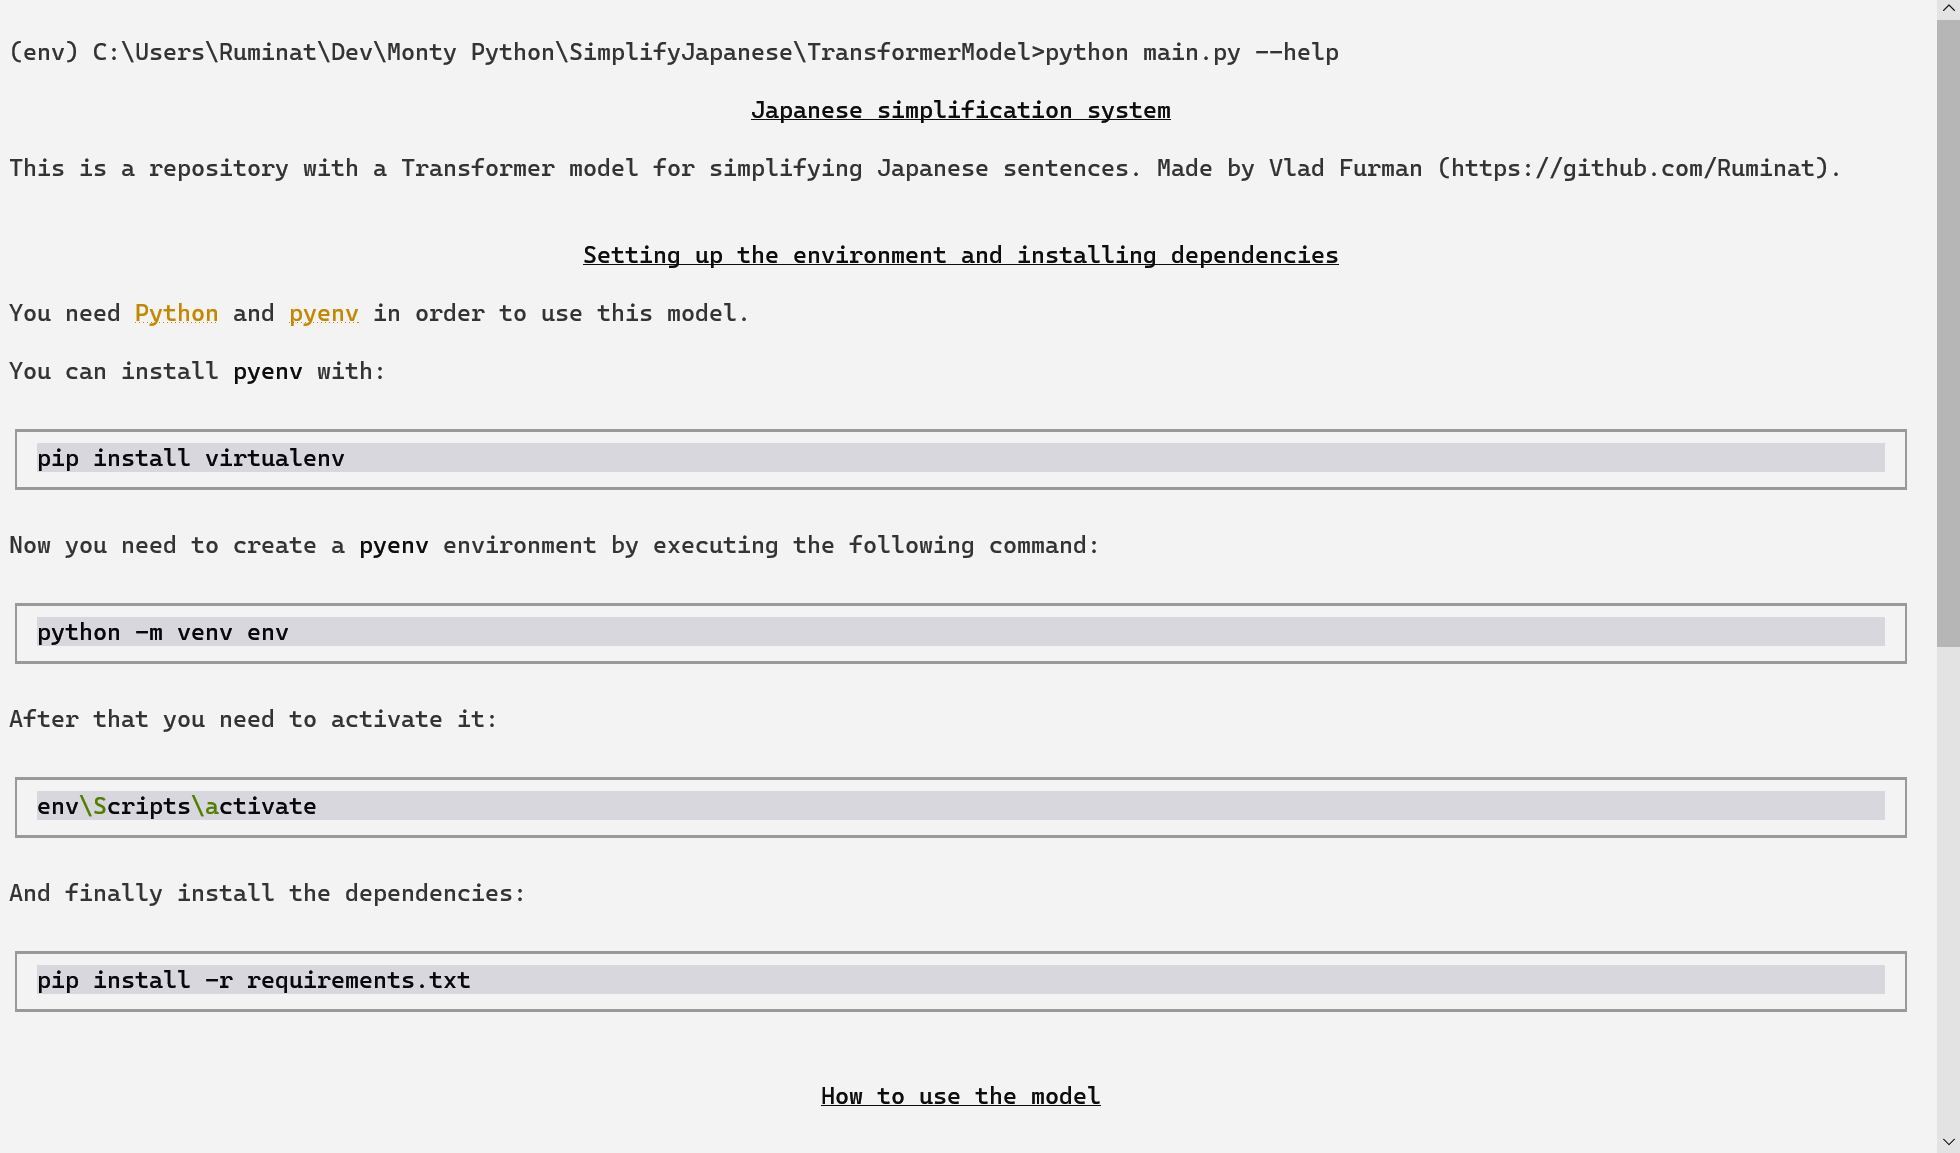
\includegraphics[width=\textwidth]{help.png}
  \caption{Частичный вывод команды \texttt{python main.py -{}-help}}
  \label{help}
\end{figure}

Поддерживаются также следующие флаги для команды \texttt{python main.py}:
\begin{enumerate}[1.]%
  \item \texttt{-{}-version} или просто \texttt{-{}-v} "--- выводит текущую версию системы,
  \item \texttt{-{}-no-print}  "--- отключает вывод упрощения тестовых предложений.
\end{enumerate}


% .---|||___|||--- S E C T I O N ---|||___|||---. %
\section{Сервер}
% .---|||___|||--- S E C T I O N ---|||___|||---. %


Как уже было сказано ранее, сервер использует фреймворк Falcon.
Имеется лишь один путь "--- \texttt{/processJapaneseText}, по которму пользовательское приложение передаёт запрос с японским текстом, после чего сервер, используя функции \texttt{getMeCabTokens}~и~\texttt{transformer.translate}, упрощает это предложение и возвращает результат приложению.


% .---|||___|||--- S U B S E C T I O N ---|||___|||---. %
\subsection{Настройка сервера}
% .---|||___|||--- S U B S E C T I O N ---|||___|||---. %


Чтобы использовать сервер, его необходимо сначала настроить.
Весь процесс подготовки окружения для сервера описан в \texttt{README.md} репозитория~\cite{ServerGithub}.
Нужно сделать следующее:
\begin{enumerate}[1.]%
  \item \texttt{pip install virtualenv} "--- установить virtual env,
  \item \texttt{python -m venv env} "--- создать virtual env,
  \item \texttt{env\textbackslash{}Scripts\textbackslash{}activate} "--- активировать virtual env,
  \item \texttt{pip install -r requirements.txt} "--- установить необходимые зависимости.
\end{enumerate}

Теперь сервер может быть запущен командами:
\begin{itemize}%
  \item \texttt{python main.py -{}-server} "--- в режиме разработки,
  \item \texttt{waitress-serve -{}-port=8000 server:app} "--- в production-окружении.
\end{itemize}


% .---|||___|||--- S U B S E C T I O N ---|||___|||---. %
\subsection{Как «общаться» с сервером}
% .---|||___|||--- S U B S E C T I O N ---|||___|||---. %


Как уже было сказано ранее, сервер имеет путь \texttt{/processJapaneseText}.
Вот пример запроса по этому пути через консольную утилиту \texttt{curl}: \\ 
\texttt{curl http://localhost:5000/processJapaneseText?text=\jp{お前はもう死んでいる}} \\ 
Пример ответа показан на~\firef{response}, где можно увидеть, что возвращается JSON со следующими полями:
\begin{itemize}%
  \item \texttt{originalText} "--- исходное предложение,
  \item \texttt{simplifiedText} "--- упрощённое предложение,
  \item \texttt{originalTextTokens} "--- исходные токены с частями речи,
  \item \texttt{simplifiedTextTokens} "--- упрощённые токены с частями речи.
\end{itemize}
\begin{figure}[H]%
  \centering
  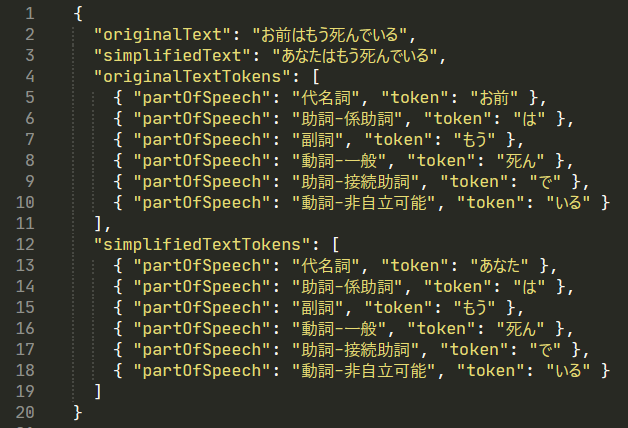
\includegraphics[height=8cm]{response.png}
  \caption{Пример ответа на запрос \texttt{/processJapaneseText}}
  \label{response}
\end{figure}


% .---|||___|||--- S E C T I O N ---|||___|||---. %
\section{Пользовательское приложение}
% .---|||___|||--- S E C T I O N ---|||___|||---. %


Пользовательское приложение выглядит довольно минималистично "--- есть форма ввода предложения, после нажатия на кнопку «Simplify» или нажатия «Ctrl»~+~«Enter» отправляется запрос на сервер (по пути \texttt{/processJapaneseText}), после чего ответ отображается в виде, как на~\firef{app-screen}.

Есть также возможность посмотреть перевод предложений (исходного и упрощённого) "--- при нажатии на ссылку «translation» открывается страница Google Translate с выбранным предложением "--- это может использоваться как некая опорная линия упрощения (что смысл не потерялся).

Цвета в предложениях (исходном и упрощённом) на~\firef{app-screen} указывают на часть речи какого-либо токена (слова).

\begin{figure}[H]%
  \centering
  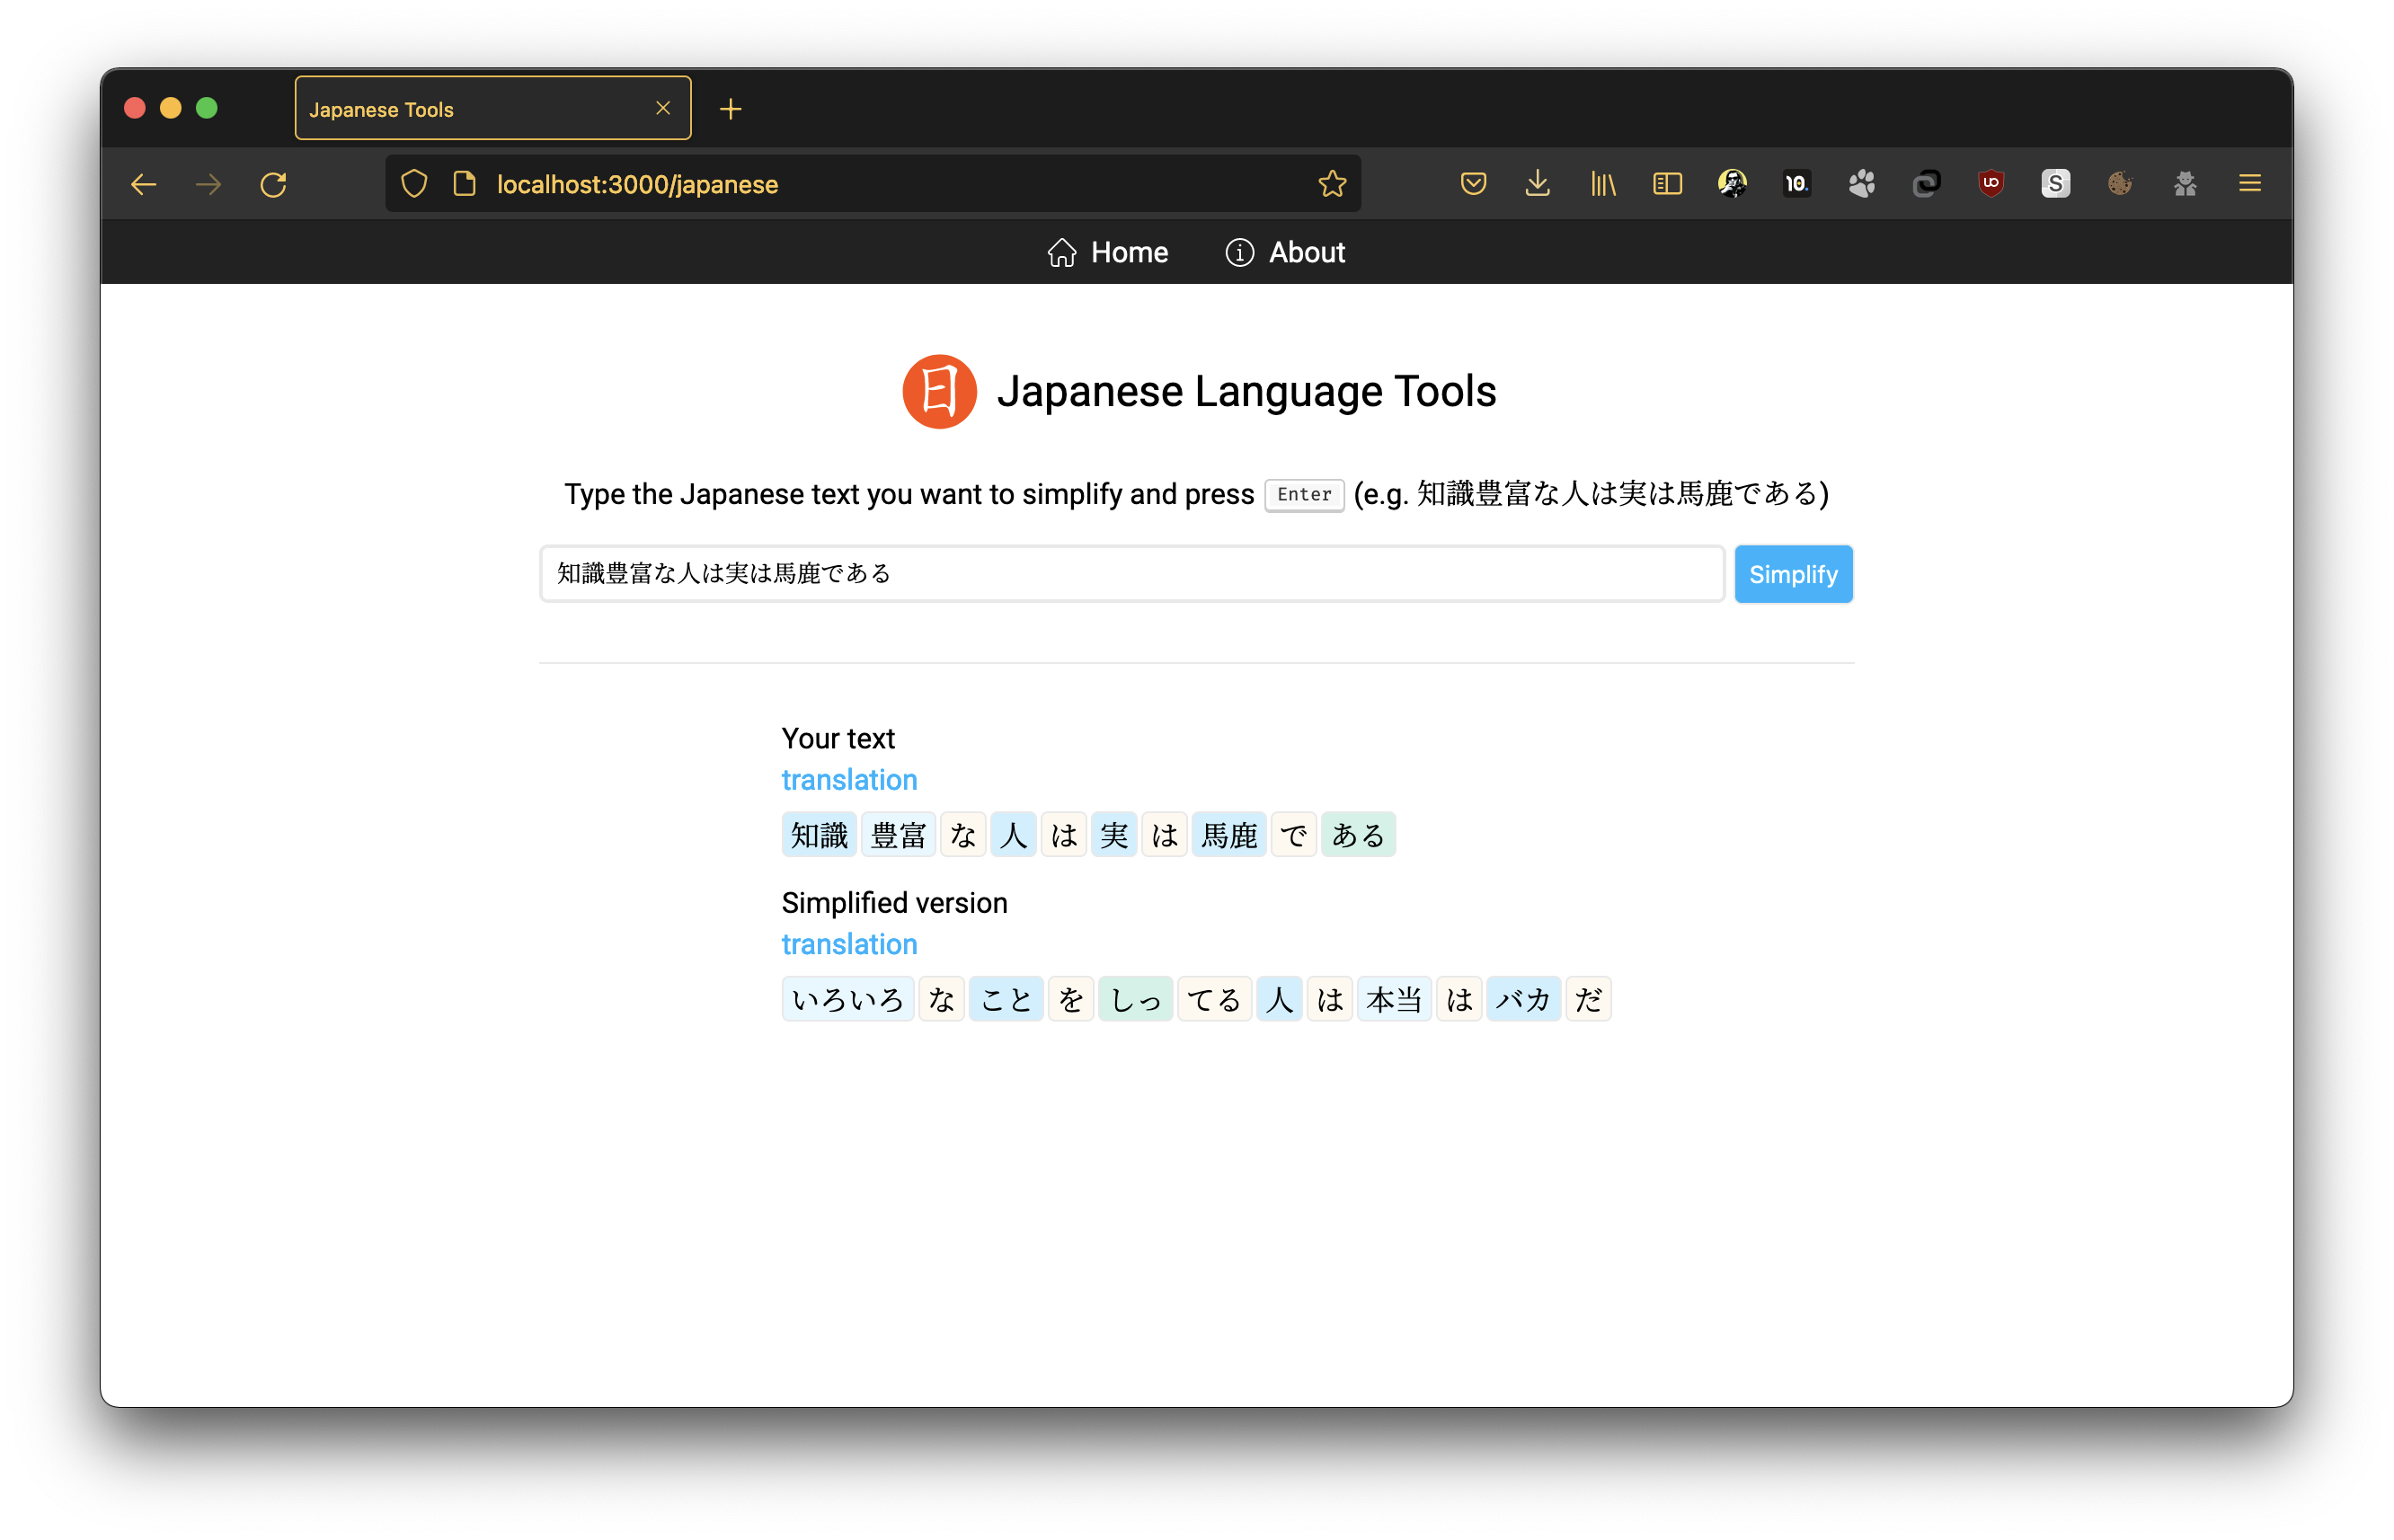
\includegraphics[width=\textwidth]{app.png}
  \caption{Пользовательское приложение}
  \label{app-screen}
\end{figure}
             % Глава 3
% %!TeX root = ../My_thesis.tex


% .---|||___|||--- C H A P T E R ---|||___|||---. %
\chapter{Аппробация разработанной модели и её модификаций}
% .---|||___|||--- C H A P T E R ---|||___|||---. %


% .---|||___|||--- S E C T I O N ---|||___|||---. %
\section{Метрики для оценки модели упрощения}
% .---|||___|||--- S E C T I O N ---|||___|||---. %


Для перевода текстов (в том числе и упрощения) довольно часто используют метрку BLEU~\cite{BLEU}.
В оригинальной статье Папинени и др. показали наличие корреляции данной метрики с сохранением грамматики и смысла переведённых предложений.

Однако есть и более специфичная метрика, разработанная специально для автоматического упрощения текстов "--- SARI~\cite{SARI}.
Она, по сравнению BLEU, лучше коррелирует с упрощением предложений, а также с сохранением лексической и структурной частей предложений.


% .---|||___|||--- S E C T I O N ---|||___|||---. %
\section{Результаты}
% .---|||___|||--- S E C T I O N ---|||___|||---. %


Результаты метрик BLUE и SARI для изначальной модели и вариантов её улучшения представлены в~\taref{metrics}.

\begin{table}[H]% Пример оформления таблицы
  \centering\small
  \caption{Метрики полученных моделей}
  \label{metrics}
    \begin{tabular}{|l|l|l|}
      \hline
      \textbf{Модель} & \textbf{BLEU} & \textbf{SARI} \\ \hline
      Transformer & 46{,}98 & 64{,}57 \\ \hline
      Pretrained Transformer & 51{,}12 & 67{,}89 \\ \hline
      Pretrained Encoder & 48{,}22 & 65{,}67 \\ \hline
    \end{tabular}
    \normalsize
\end{table}

В~\taref{metrics} введены следующие обозначения:
\begin{itemize}%
  \item Transformer "--- изначальная модель;
  \item Pretrained Transformer "--- предобученная модель, которую дообучаем, замедляя обучение encoder'а;
  \item Pretrained Encoder "--- изначальная модель, в которой заменяем encoder на предобученный, замедляя его обучение.
\end{itemize}

По~\taref{metrics} видно, что наиболее успешной оказалсь модель Pretrained Transformer "--- улучшение по сравнению с изначальной моделью на 4{,}14\% и 3{,}32\% для BLEU и SARI соответственно.
Это может говорить о том, что предобучение положительно сказывается и на decoder'е, так как упрощение в основном оставляет предложение в исходном виде, за исключением упрощённых его частей.


% .---|||___|||--- S E C T I O N ---|||___|||---. %
\section{Гистограммы и доверительные интервалы}
% .---|||___|||--- S E C T I O N ---|||___|||---. %


Рассмотрим гистограммы распределения значений метрик BLUE и SARI для изначальной модели (Transformer) и улучшенной версии (Pretrained Transformer) "--- см.~\firef{metrics-comparison}.
Можно увидеть, как в левой части гистограмм (худшие показатели метрик) доминирует первая модель, на правой же части (лучшие показатели метрик) "--- модифицированная.

\begin{figure}[H]%
  \centering%
  \caption{Сравнение гистограмм метрик BLEU~(a) и SARI~(b) \\ жёлтый "--- Transformer, синий "--- Pretrained Transformer}
  \label{metrics-comparison}
  \begin{subfigure}[H]{0.45\textwidth}
    \label{bleu-part}
    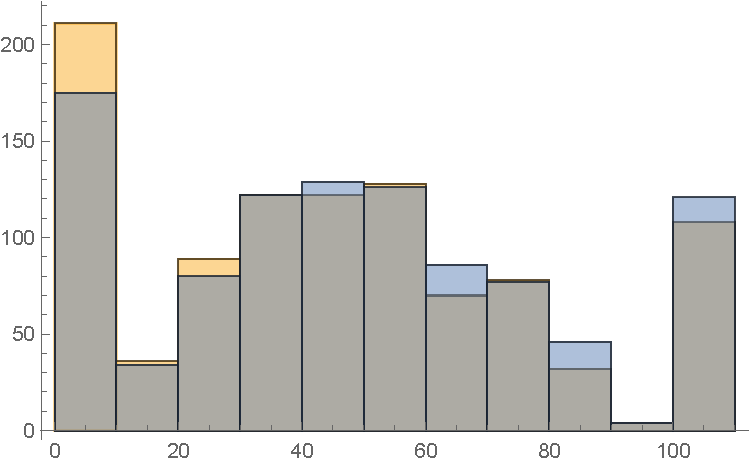
\includegraphics[width=\textwidth]{bleu-comparison.pdf}
    \caption{Метрики BLEU}
  \end{subfigure}
  \begin{subfigure}[H]{0.45\textwidth}
    \label{sari-part}
    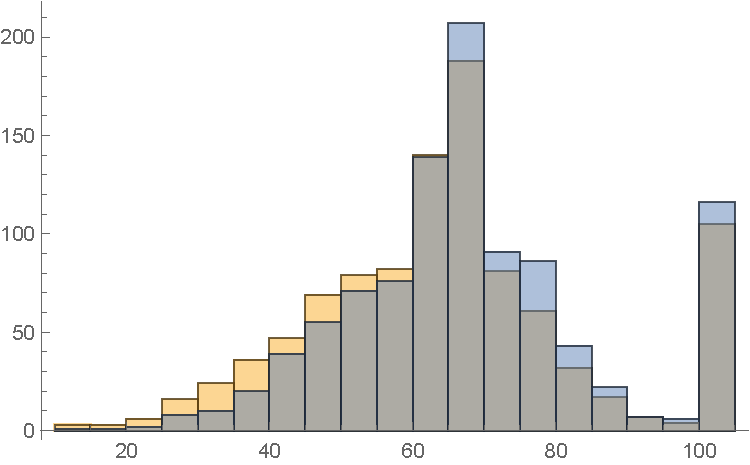
\includegraphics[width=\textwidth]{sari-comparison.pdf}
    \caption{Метрики SARI}
  \end{subfigure}
\end{figure}%

Это может говорить о том, что улучшение модели действительно положительно влияет на полученные показания метрик, однако для большей уверенности в этой гипотезе вычислим доверительные интервалы для этих значений и посмотрим, не пересекаются ли они. Доверительные интервалы (Confidence Intervals, CI) могут быть вычислены по формуле~\eqref{ci-formula}.

\begin{equation}%
  \label{ci-formula}
  CI = \mu \pm p \frac{\sigma}{\sqrt{N}},
\end{equation}
где
\begin{itemize}%
  \item $CI$ "--- доверительные интервалы,
  \item $\mu$ "--- среднее значение выборки,
  \item $p$ "--- вероятность попадания истинного значения в доверительные интервалы (в данной работе возьмём значение $0{,}95$),
  \item $\sigma$ "--- среднеквадратическое отклонение выборки,
  \item $N$ "--- количество элементов в выборке (в данной работе "--- 1\,000).
\end{itemize}

Вычислим доверительные интервалы:~\eqref{bleu-ci}~и~\eqref{sari-ci}\footnote{Заметим, что среднее значение для метрик BLEU отличается от указанных значений в~\taref{metrics}. Связано это с тем, что метрика BLEU вычисляется иным образом для набора предложений, в отличие от единичных предложений, однако разность между значениями при единичных вычислениях ниже, в то время как доверительные интервалы не пересекаются, что говорит о том, что и доверительные интервалы для значений со всеми предложениями не пересекаются. В случае же с SARI разницы никакой нет.}.

\begin{equation}\label{bleu-ci}%
  CI_{\text{Transformer (BLEU)}} = 43{,}85 \pm 0{,}95, \
  CI_{\text{Pretrained Transformer (BLEU)}} = 47{,}37 \pm 0{,}94,
\end{equation}

\begin{equation}\label{sari-ci}%
  CI_{\text{Transformer (SARI)}} = 64.5686 \pm 0{,}55, \
  CI_{\text{Pretrained Transformer (SARI)}} = 67.89 \pm 0{,}51.
\end{equation}

В итоге получаем расстояние между нижней границей Pretrained Transformer и верхней границей Transformer в $1{,}63$ и $2{,}26$ для метрик BLEU и SARI соответственно, что может говорить о явном различии истинных значений метрик BLUE и SARI для изначальной и модифицированной моделей.
А это, в свою очередь, говорит о наличии значимости внесённых изменений в модель со статистической точки зрения.


% .---|||___|||--- S E C T I O N ---|||___|||---. %
\section{Примеры упрощения предложений изначальной и модифицированной моделями}
% .---|||___|||--- S E C T I O N ---|||___|||---. %


Рассмотрим примеры предложений из корпуса для тестирования, упрощение которых улучшилось благодаря модификции модели "--- см.~\firef{simplificationComparison}\footnote{Здесь также происходит упрощение слова \jp{ますます} (на \jp{さらに} "--- более распространённое слово), однако обе модели упростили его одинакого, поэтому не будем заострять на этом внимание.}.

\begin{figure}[H]%
  \centering
  \begin{tabular}{l}
    (1) исходное предложение \\  
    \yubi{\jp{彼女}}{kanojo}
    \yubi{\jp{は}}{wa}
    \yubi{\jp{内気}}{uchiki}
    \yubi{\jp{な}}{na}
    \yubi{\jp{ので}}{node}
    \yubi{\jp{、}}{}
    \yubi{\jp{ますます}}{masumasu}
    \yubi{\jp{彼女}}{kanojo}
    \yubi{\jp{が}}{ga}
    \yubi{\jp{好き}}{suki}
    \yubi{\jp{だ}}{da} \\ 
    пер. "--- она робкая, из-за чего я люблю её ещё больше \\ 
    (2) изначальная модель \\ 
    \yubi{\jp{彼女}}{kanojo}
    \yubi{\jp{は}}{wa}
    \yubi{\jp{弱い}}{\textbf{yowai}}
    \yubi{\jp{ので}}{node}
    \yubi{\jp{、}}{}
    \yubi{\jp{さら}}{sara}
    \yubi{\jp{に}}{ni}
    \yubi{\jp{彼女}}{kanojo}
    \yubi{\jp{が}}{ga}
    \yubi{\jp{好き}}{suki}
    \yubi{\jp{だ}}{da} \\ 
    пер. "--- она \textbf{слабая}, из-за чего я люблю её ещё больше \\ 
    (3) модифицированная модель (Pretrained Transformer) \\  
    \yubi{\jp{彼女}}{kanojo}
    \yubi{\jp{は}}{wa}
    \yubi{\jp{気}}{\textbf{ki}}
    \yubi{\jp{が}}{\textbf{ga}}
    \yubi{\jp{弱い}}{\textbf{yowai}}
    \yubi{\jp{ので}}{node}
    \yubi{\jp{、}}{}
    \yubi{\jp{さら}}{sara}
    \yubi{\jp{に}}{ni}
    \yubi{\jp{彼女}}{kanojo}
    \yubi{\jp{が}}{ga}
    \yubi{\jp{好き}}{suki}
    \yubi{\jp{だ}}{da} \\
    пер. "--- она \textbf{скромная}, из-за чего я люблю её ещё больше \\ 
  \end{tabular}
  \caption{Пример улучшения упрощения предложения \\ \jp{彼女は内気なので、ますます彼女が好きだ}}
  \label{simplificationComparison}
\end{figure}

Рассмотрим ещё один пример "--- см.~\firef{simplificationComparison2}.
Здесь есть непереводимый на русский язык нюанс упрощения "--- \jp{我}~(литературное «я»)~$\to$~\jp{自分}~(обычное «я»)\footnote{Это именно тот самый случай многообразия японских местоимений (о котором мы говорили в первой главе), каждое из которых несёт свой оттенок и имеет своё место в использовании в японском языке, в русском же языке есть лишь одно слово "--- «я».}.
Заметим также, что в изначальной модели искажается исходный смысл предложения (хотя предложение и упрощается), в модифицированной же модели этот смысл сохраняется (упрощение также производится).

\begin{figure}[H]%
  \centering
  \begin{tabular}{l}
    (1) исходное предложение \\  
    \yubi{\jp{彼}}{kare}
    \yubi{\jp{は}}{wa}
    \yubi{\jp{怒り}}{okori}
    \yubi{\jp{に}}{ni}
    \yubi{\jp{我}}{ware}
    \yubi{\jp{を}}{wo}
    \yubi{\jp{忘れた}}{wasureta} \\ 
    пер. "--- он забылся в гневе \\ 
    (2) изначальная модель \\ 
    \yubi{\jp{彼}}{kare}
    \yubi{\jp{は}}{wa}
    \yubi{\jp{怒っている}}{okotteiru}
    \yubi{\jp{のに}}{noni}
    \yubi{\jp{自分}}{\textbf{jibun}}
    \yubi{\jp{の}}{no}
    \yubi{\jp{意見}}{\textbf{iken}}
    \yubi{\jp{を}}{\textbf{wo}}
    \yubi{\jp{忘れた}}{\textbf{wasureta}} \\ 
    пер. "--- он хоть и разозлился, но \textbf{забыл своё мнение} \\ 
    (3) модифицированная модель (Pretrained Transformer) \\  
    \yubi{\jp{彼}}{kare}
    \yubi{\jp{は}}{wa}
    \yubi{\jp{怒っている}}{okotteiru}
    \yubi{\jp{こと}}{koto}
    \yubi{\jp{に}}{ni}
    \yubi{\jp{自分}}{\textbf{jibun}}
    \yubi{\jp{を}}{wo}
    \yubi{\jp{忘れた}}{wasureta} \\ 
    пер. "--- он забылся, из-за того что разозлился \\ 
  \end{tabular}
  \caption{Пример улучшения упрощения предложения \\ \jp{彼は怒りに我を忘れた}}
  \label{simplificationComparison2}
\end{figure}


% % .---|||___|||--- S E C T I O N ---|||___|||---. %
% \section{Примеры упрощения разработанной системой}
% % .---|||___|||--- S E C T I O N ---|||___|||---. %


% Посмотрим на несколько примеров упрощения разработанной системой, а также улучшенной версии.


             % Глава 3
% \ContinueChapterEnd % завершить размещение глав <<подряд>>
% %% Завершение основной части

%!TeX root = ../Asq.tex
\begin{frame}{Заключение}%
  \begin{itemize}%
    \item Была изучена предметная область,
    \item были исследованы методы анализа и формализации русского языка,
    \item была разработана система трансляции запросов на русском языке в SQL-код,
    \item разработанная система была протестирована на запросах различной сложности.
  \end{itemize}
\end{frame}
           % Заключение

% %% Наличие следующих перечней не исключает расшифровку сокращения и условного обозначения при первом упоминании в тексте!
% \chapter*{Список сокращений и условных обозначений}             % Заголовок
\addcontentsline{toc}{chapter}{Список сокращений и условных обозначений}  % Добавляем его в оглавление
\noindent
\addtocounter{table}{-1}% Нужно откатить на единицу счетчик номеров таблиц, так как следующая таблица сделана для удобства представления информации по ГОСТ
%\begin{longtabu} to \dimexpr \textwidth-5\tabcolsep {r X}
\begin{longtabu} to \textwidth {r X}
% Жирное начертание для математических символов может иметь
% дополнительный смысл, поэтому они приводятся как в тексте
% диссертации
$\begin{rcases}
a_n\\
b_n
\end{rcases}$  & 
\begin{minipage}{\linewidth}
коэффициенты разложения Ми в дальнем поле соответствующие
электрическим и магнитным мультиполям
\end{minipage}
\\
${\boldsymbol{\hat{\mathrm e}}}$ & единичный вектор \\
$E_0$ & амплитуда падающего поля\\
$\begin{rcases}
a_n\\
b_n
\end{rcases}$  & 
коэффициенты разложения Ми в дальнем поле соответствующие
электрическим и магнитным мультиполям ещё раз, но без окружения
minipage нет вертикального выравнивания по центру.
\\
$j$ & тип функции Бесселя\\
$k$ & волновой вектор падающей волны\\

$\begin{rcases}
a_n\\
b_n
\end{rcases}$  & 
\begin{minipage}{\linewidth}
\vspace{0.7em}
и снова коэффициенты разложения Ми в дальнем поле соответствующие
электрическим и магнитным мультиполям, теперь окружение minipage есть
и добавленно много текста, так что описание группы условных
обозначений значительно превысило высоту этой группы... Для отбивки
пришлось добавить дополнительные отступы.
\vspace{0.5em}
\end{minipage}
\\
$L$ & общее число слоёв\\
$l$ & номер слоя внутри стратифицированной сферы\\
$\lambda$ & длина волны электромагнитного излучения
в вакууме\\
$n$ & порядок мультиполя\\
$\begin{rcases}
{\mathbf{N}}_{e1n}^{(j)}&{\mathbf{N}}_{o1n}^{(j)}\\
{\mathbf{M}_{o1n}^{(j)}}&{\mathbf{M}_{e1n}^{(j)}}
\end{rcases}$  & сферические векторные гармоники\\
$\mu$  & магнитная проницаемость в вакууме\\
$r,\theta,\phi$ & полярные координаты\\
$\omega$ & частота падающей волны\\

  \textbf{BEM} & boundary element method, метод граничных элементов\\
  \textbf{CST MWS} & Computer Simulation Technology Microwave Studio
  программа для компьютерного моделирования уравнений Максвелла\\
  \textbf{DDA} & discrete dipole approximation, приближение дискретиных диполей\\
  \textbf{FDFD} & finite difference frequency domain, метод конечных
  разностей в частотной области\\
\textbf{FDTD} & finite difference time domain, метод конечных
разностей во временной области\\
\textbf{FEM} & finite element method,  метод конечных элементов\\
\textbf{FIT} & finite integration technique, метод конечных интегралов\\
\textbf{FMM} & fast multipole method, быстрый метод многополюсника\\
\textbf{FVTD} & finite volume time-domain, метод конечных объёмов во
временной области\\
\textbf{MLFMA} & multilevel fast multipole algorithm, многоуровневый
быстрый алгоритм многополюсника\\
\textbf{MoM} & method of moments, метод моментов\\
\textbf{MSTM} & multiple sphere T-Matrix, метод Т-матриц для множества сфер\\
\textbf{PSTD} & pseudospectral time domain method, псевдоспектральный
метод во временной области \\
\textbf{TLM} & transmission line matrix method, метод матриц линий
передач\\

\end{longtabu}
             % Необязательная рубрика! Список сокращений и условных обозначений

% \chapter*{Словарь терминов}             % Заголовок
\addcontentsline{toc}{chapter}{Словарь терминов}  % Добавляем его в оглавление

\textbf{TeX} --- язык вёрстки текста и издательская система, разработанные Дональдом Кнутом.

\textbf{LaTeX} --- язык вёрстки текста и издательская система, разработанные Лэсли Лампортом как надстройка над TeX.

         % Необязательная рубрика! Словарь терминов
% По порядку после Списка сокращений и условных обозначений, если есть. 


%%% Не мянять - Do not modify
%%
%%
\clearpage                                  % В том числе гарантирует, что список литературы в оглавлении будет с правильным номером страницы
%\hypersetup{ urlcolor=black }               % Ссылки делаем чёрными
%\providecommand*{\BibDash}{}                % В стилях ugost2008 отключаем использование тире как разделителя 
\urlstyle{rm}                               % ссылки URL обычным шрифтом
\ifdefmacro{\microtypesetup}{\microtypesetup{protrusion=false}}{} % не рекомендуется применять пакет микротипографики к автоматически генерируемому списку литературы
%\newcommand{\fullbibtitle}{Список литературы} % (ГОСТ Р 7.0.11-2011, 4)
%\insertbibliofull  
%\noindent
%\begin{group}
\chapter*{Список использованных источников}	
\label{references}
\addcontentsline{toc}{chapter}{Список использованных источников}	% в оглавление 
\printbibliography[env=SSTfirst]                         % Подключаем Bib-базы
%\ifdefmacro{\microtypesetup}{\microtypesetup{protrusion=true}}{}
%\urlstyle{tt}                               % возвращаем установки шрифта ссылок URL
%\hypersetup{ urlcolor={urlcolor} }          % Восстанавливаем цвет ссылок



%\urlstyle{rm}                               % ссылки URL обычным шрифтом
%\ifdefmacro{\microtypesetup}{\microtypesetup{protrusion=false}}{} % не рекомендуется применять пакет микротипографики к автоматически генерируемому списку литературы
%\insertbibliofull                           % Подключаем Bib-базы
%\ifdefmacro{\microtypesetup}{\microtypesetup{protrusion=true}}{}
%\urlstyle{tt}                               % возвращаем установки шрифта ссылок URL
         % Список литературы

% Здесь можно поместить список иллюстративного материала

\appendix % не редактировать / keep unmodified


% \chapter{Исходный код}\label{appendix-code}							% Заголовок
%\addcontentsline{toc}{chapter}{Second call for chapters to participate in the book Machine learning in analysis of biomedical and socio-economic data}	% Добавляем его в оглавление

\newcommand{\sourceCodeFile}[2]{%
	Файл \texttt{#1} (#2):
	\inputminted[tabsize=2, mathescape, fontsize=\fontsize{10}{10}\selectfont]{python}{code/#1}%
}

\sourceCodeFile{main.py}{главный файл для запуска обучения модели или старта сервера}
\sourceCodeFile{definitions.py}{основные определения и константы}
\sourceCodeFile{utils.py}{утилиты для запуска модели}

\sourceCodeFile{apps/SimplificationServer/main.py}{сервер на Falcon}
\sourceCodeFile{modules/Parser/definitions.py}{MeCab-токен}
\sourceCodeFile{modules/Parser/utils.py}{токенизация через MeCab}

\sourceCodeFile{apps/Transformer/main.py}{запуск обучения/загрузки модели из сохраннёного файла из директории \texttt{/build}}

\sourceCodeFile{modules/Seq2SeqTransformer/main.py}{модель sequence2sequence Transformer "--- финальная модель для упрощения}
\sourceCodeFile{modules/Seq2SeqTransformer/utils.py}{утилиты для обучения модели упрощения}

\sourceCodeFile{modules/PositionalEncoding/main.py}{модель positional encoding}

\sourceCodeFile{modules/Embedding/main.py}{модель эмбеддингов}

\sourceCodeFile{modules/Language/definitions.py}{определения языков}
\sourceCodeFile{modules/Language/utils.py}{утилиты для обработки языков}

\sourceCodeFile{modules/Dataset/main.py}{класс корпуса}
\sourceCodeFile{modules/Dataset/definitions.py}{типы для корпусов}
\sourceCodeFile{modules/Dataset/snowSimplifiedJapanese/main.py}{корпус упрощения предложений на японском языке SNOW (T15 и T23)}

% \sourceCodeFile{modules/Metrics/bleu.py}{метрика BLEU}
% \sourceCodeFile{modules/Metrics/sari.py}{метрика SARI}

% \begin{minted}[tabsize=2, mathescape, linenos, xleftmargin=20pt, fontsize=\scriptsize]{python}
% def scaledDotProductAttention(
%   query: Tensor,
%   key: Tensor,
%   value: Tensor,
%   mask: Optional[Tensor] = None
% ) -> Tensor:
%   # Считаем scale, на который будем делить
%   scale = query.size(-1) ** 0.5
%   # Перемножаем матрицы query и key, делим их на scale
%   temp = query.bmm(key.transpose(1, 2)) / scale

%   # Применяем маску, если она есть
%   if (mask is not None):
%     temp += mask

%   # Применяем softmax к измерению embedding'ов
%   softmax = f.softmax(temp, dim=-1)
%   # Перемножаем softmax с матрицей value
%   return softmax.bmm(value)
% \end{minted}
          % Приложение 1

% \chapter{Некоторые дополнительные примеры}\label{appendix-extra-examples}							% 

В приложении\footnote{Внимание! Пример оформления подстрочной ссылки (сноски).} приведены формулы \eqref{eq:Pi-app}, \eqref{eq:Pi-app-}, \firef{fig:spbpu_hydrotower-app}, \firef{fig:spbpu_hydrotower-app-}, \taref{tab:ToyCompare-app}, \taref{tab:ToyCompare-app-}


\begin{equation}% лучше не оставлять пропущенную строку (\par) перед окружениями для избежания лишних отсупов в pdf
\label{eq:Pi-app-} % eq - equations, далее название, ch поставлено для избежания дублирования
\pi \approx 3,141.
\end{equation}
%
%
\begin{figure}[ht!] 
	\center
	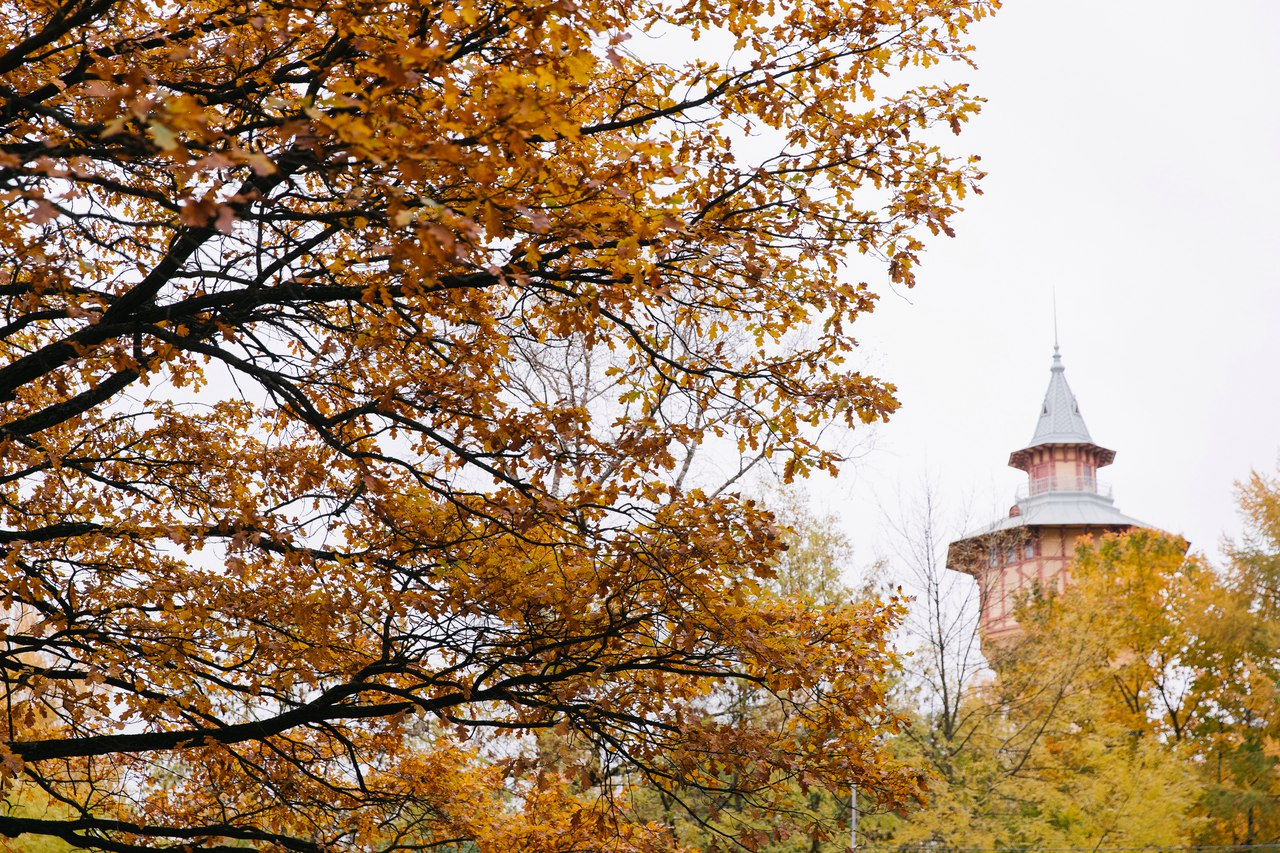
\includegraphics [scale=0.27] {my_folder/images//spbpu_hydrotower}
	\caption{Вид на гидробашню СПбПУ \cite{spbpu-gallery}} 
	\label{fig:spbpu_hydrotower-app-}  
\end{figure}

\begin{table} [htbp]% Пример оформления таблицы
	\centering\small
	\caption{Представление данных для сквозного примера по ВКР \cite{Peskov2004}}%
	\label{tab:ToyCompare-app-}		
	\begin{tabular}{|l|l|l|l|l|l|}
		\hline
		$G$&$m_1$&$m_2$&$m_3$&$m_4$&$K$\\
		\hline
		$g_1$&0&1&1&0&1\\ \hline
		$g_2$&1&2&0&1&1\\ \hline
		$g_3$&0&1&0&1&1\\ \hline
		$g_4$&1&2&1&0&2\\ \hline
		$g_5$&1&1&0&1&2\\ \hline
		$g_6$&1&1&1&2&2\\ \hline		
	\end{tabular}	
	\normalsize% возвращаем шрифт к нормальному
\end{table}




\section{Подраздел приложения}\label{app-2-1}							


\begin{equation}% лучше не оставлять пропущенную строку (\par) перед окружениями для избежания лишних отсупов в pdf
\label{eq:Pi-app} % eq - equations, далее название, ch поставлено для избежания дублирования
\pi \approx 3,141.
\end{equation}
%
%
\begin{figure}[ht!] 
	\center
	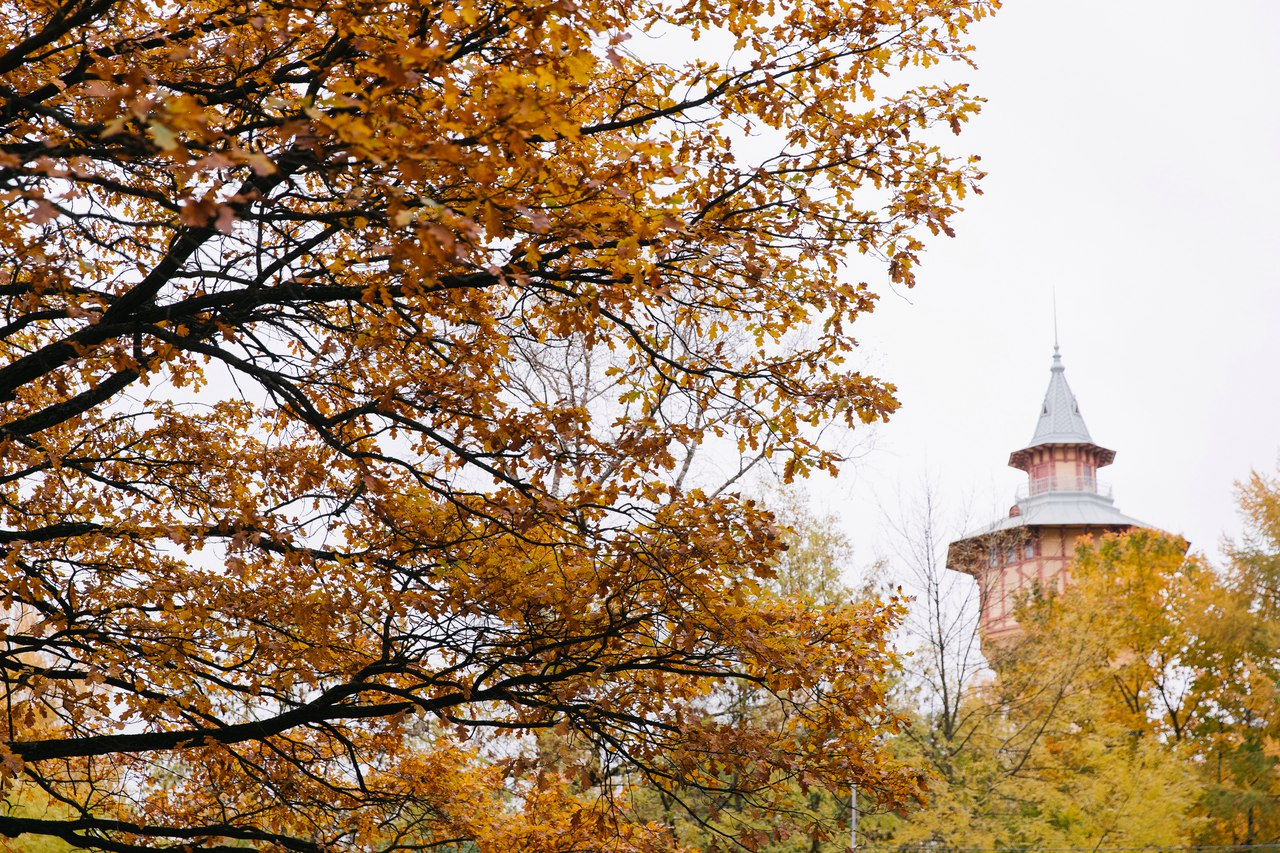
\includegraphics [scale=0.27] {my_folder/images//spbpu_hydrotower}
	\caption{Вид на гидробашню СПбПУ \cite{spbpu-gallery}} 
	\label{fig:spbpu_hydrotower-app}  
\end{figure}

\begin{table} [htbp]% Пример оформления таблицы
	\centering\small
	\caption{Представление данных для сквозного примера по ВКР \cite{Peskov2004}}%
	\label{tab:ToyCompare-app}		
	\begin{tabular}{|l|l|l|l|l|l|}
		\hline
		$G$&$m_1$&$m_2$&$m_3$&$m_4$&$K$\\
		\hline
		$g_1$&0&1&1&0&1\\ \hline
		$g_2$&1&2&0&1&1\\ \hline
		$g_3$&0&1&0&1&1\\ \hline
		$g_4$&1&2&1&0&2\\ \hline
		$g_5$&1&1&0&1&2\\ \hline
		$g_6$&1&1&1&2&2\\ \hline		
	\end{tabular}	
	\normalsize% возвращаем шрифт к нормальному
\end{table}

        % Приложение 2


\end{document} % конец документа


%%% Удачной защиты ВКР! - Good luck on the thesis defense!
%%
%%% Поддержать проект
%%
%% Запросы на добавление / изменение просим писать на следующей странице:
%% https://github.com/ParkhomenkoV/SPbPU-student-thesis-template/issues
%%
%% Список пожеланий в файле шаблона <<TO-DO-list.tex>>
%%
%% Благодарности просим указывать в виде 
%%
%% 1. Добавление <<Звезды>> проекту https://github.com/ParkhomenkoV/SPbPU-student-thesis-template/stargazers
%%
%% 2. Добавления <<Сердечка>> и репоста проекта в социальных сетях:
%%    https://vk.com/latex_polytech 
%%    https://www.fb.com/groups/latex.polytech
%%

%%% Support project
%%
%% Requests on adding / modifications is better to be publishen on the following web-page:
%% https://github.com/ParkhomenkoV/SPbPU-student-thesis-template/issues
%%
%% Wishlist is in the template's file called <<TO-DO-list.tex>>
%%
%% Acknowledgements are better to be done in the form of 
%%
%% 1. Adding <<Star>> to the project https://github.com/ParkhomenkoV/SPbPU-student-thesis-template/stargazers
%%
%% 2. Adding <<Likes>> and Project repost in the social networks:
%%    https://vk.com/latex_polytech 
%%    https://www.fb.com/groups/latex.polytech
%% 

% Check list при передаче ВКР:
% - Количество страниц в Задании 2. Если нет, то комментирование последней строки в my_task.tex
% - Зачистка всех вспомогательных файлов (Clear auxilary files) и компиляция ВКР не менее 3х раз